\documentclass[10pt,twoside,a4paper,fleqn]{report}
\usepackage{etex} % required for tikz figures

\usepackage{amsmath}

\usepackage{graphicx}
\usepackage{caption}
\usepackage{subcaption}

\usepackage{array}
\usepackage{amssymb}
\usepackage{pifont}
\usepackage{xcolor}
\usepackage{siunitx}


\usepackage[english,mt]{rpg} % select type {semester}/bachelor/master thesis: {st}/bt/mt

% Page header (don't change)____________________________________________________
\setlength{\parindent}{0em}                 % Disable parindent
\rhead[\nouppercase{\rightmark}]{\thepage}  % Special headings
\lhead[\thepage]{\nouppercase{\leftmark}}   % Special headings
\cfoot{}                                    % Special headings

%%%%%%%% Hint %%%%%%%%%%%
% Define your custom stuff here, e.g. Symbols that you are using. If you define them here it is easy to change them later on if you run into a nomenclature conflict.
\newcommand{\mysymbol}[0]{\mathbf{S}_{my}}   % custom symbol which can easily be changed if necessary
\newcommand{\bomega}[0]{\boldsymbol{\omega}} % bold greek letter
\newcommand{\bSymb}[1]{\mathbf{#1}}			% toy example with one argument
\newcommand\ddfrac[2]{\frac{\displaystyle #1}{\displaystyle #2}}

% tikz plots
\pgfplotsset{compat=newest}
\pgfplotsset{plot coordinates/math parser=false}
\pgfplotsset{yticklabel style={text width=2em,align=right}}
\newlength\fheight
\newlength\fwidth

% Figures from Inkscape
\graphicspath{{img//}}

% Title page (please fill in)___________________________________________________
\title{Autonomous Quadrotor Landing on a Moving Platform with only Onboard Sensing and Computing}

\studentA{Alessio Zanchettin}
\ethidA{13-947-221}
\emailA{zalessio@student.ethz.ch}

% \studentB{Second Student}
% \ethidB{12-345-678}
% \semesterB{9}
% \emailB{second@student.ethz.ch}

\supervision{Davide Falanga\\ Junje Zhang \\ Prof. Dr. Davide Scaramuzza}
\date{September 2016}

\infopage
\declaration

% Begin document________________________________________________________________
\begin{document}
\maketitle 							      % Create title page

% Preamble______________________________________________________________________
\pagenumbering{roman} 				% Begin roman page numbering (i,ii,...)
%---------------------------------------------------------------------------
% Table of contents

 \setcounter{tocdepth}{2}
 \tableofcontents
 \cleardoublepage

%---------------------------------------------------------------------------
% List of Figures

 % \addcontentsline{toc}{chapter}{List of Figures}
 % \listoffigures
 % \clearpage

%---------------------------------------------------------------------------
% List of Tables

 % \addcontentsline{toc}{chapter}{List of Algorithms}
 % \listofalgorithms
 % \clearpage

%---------------------------------------------------------------------------
% Abstract

\chapter*{Abstract}
 \addcontentsline{toc}{chapter}{Abstract}
In this thesis we present a complete framework to autonomous landing on a moving platform
TODO complete \\
  Compress the introduction in a few key sentences. No more than half a page. The abstract should motivate your work, outline the work that you did, and give some insights into its results.

 \cleardoublepage

%---------------------------------------------------------------------------
% Symbols

\chapter*{Nomenclature}\label{chap:symbole}
\addcontentsline{toc}{chapter}{Nomenclature}

\section*{Notation}
  \begin{tabbing}
    \hspace*{1.6cm}   \= \kill
    $\mathbf{J}$       \> Jacobian \\[0.5ex]
    $\mathbf{H}$       \> Hessian \\[0.5ex]
    $\boldsymbol{r}$  \> position of the frame $B$ with respect to frame $W$ \\[0.5ex]
    $\mathbf{T}_{WB}$  \> coordinate transformation from frame $B$ to frame $W$ \\[0.5ex]
    $\mathbf{R}_{WB}$  \> orientation of $B$ with respect to $W$ \\[0.5ex]
    $_W\mathbf{t}_{WB}$\> translation of $B$ with respect to $W$, expressed in coordinate system $W$ \\[0.5ex]
    $\hat{\boldsymbol{w}_{WB}}$ \> skew symmetric matrix \\[0.5ex]
    $\boldsymbol{c}$  \> thrust vector with respect to frame $B$ \\[0.5ex]
    $\boldsymbol{g}$  \> gravity with respect to frame $W$ \\[0.5ex]
  \end{tabbing}
  
Scalars are written in lower case letters ($a$), vectors in lower case bold letters ($\mathbf{a}$) and matrices in upper case bold letters ($\mathbf{A}$).

\section*{Acronyms and Abbreviations}
  \begin{tabbing}
    \hspace*{1.6cm}  \= \kill
    RPG     \> Robotics and Perception Group \\[0.5ex]
    UAV     \> Unmanned Aerial Vehicle \\[0.5ex]
    UGV     \> Unmanned Ground Vehicle \\[0.5ex]
    MAV     \> Micro Aerial Vehicle \\[0.5ex]
    ROS     \> Robot Operating System \\[0.5ex]
    DoF     \> Degree of Freedom \\[0.5ex]
    IMU     \> Inertial Measurement Unit \\[0.5ex]
    EKF   \> Extended Kalman Filter \\[0.5ex]
    SVO   \> Semidirect Visual Odometry \\[0.5ex]
    MSF   \> Multi Sensor Fusion \\[0.5ex]
    MBZIRC    \> Mohamed Bin Zayed International Robotics Challenge \\[0.5ex]
  \end{tabbing}

\clearpage

%---------------------------------------------------------------------------


% Chapters______________________________________________________________________
\pagestyle{fancy}             % Fancy headings
\pagenumbering{arabic}				% Begin arabic page numbering (1,2,...)

\chapter{Introduction}\label{chap:introduction}
Unmanned Aerial Vehicles (UAVs) are, nowadays, accessible to all kind of users and many applications have been trying to use these vehicles in increasingly difficult settings. For many of those scenarios is necessary autonomous landing of the UAV on a small base using only on- board sensors. As a matter of fact, major drawback of current civil Micro Air Vehicles (MAVs) is the limited flight time. Automated landing systems, along with suitable recharging platforms, enable longer term UAV missions with greater autonomy. Furthermore there are several applications in which the landing target is not static, but it is moving w.r.t the world coordinate frame, so the quadrotor must be able to perform a precise landing maneuver over this moving platform, this situation would occur, for example, when landing on a moving ship or car.\\

Highly accurate localization is required in order to allow the MAV to land precisely over the platform. Most of UAVs are provided by a GPS, but this sensor can have errors up to 5 meters radius, and landing with such low-quality state estimation will have an almost certain probability of failure. Fortunately, many applications require the usage of other sensors, such as on- board cameras: vision based approaches, to state estimation, are promising in this respect.\\

In this work we present a complete framework to perform an entire landing task. The main parts of the framework are:
\begin{itemize}
\item self localization and state estimation of the UAV
\item detection, tracking and state estimation of the landing target
\item dynamic trajectory planning to perform a precise and smooth land
\end{itemize}
\section{Related Work}\label{sec:related_work}

During the last 15 years several methods where developed in order to achieve automatic landing for UAVs.
usually, in these projects calculations are done by the ground station, which allows great processing power, but leads to restrictions in autonomy on the UAV. \\

At the beginning the research was about landing on a static platform. Hardware and tequinques used to achive the succesful completement of the task were various.

Some of them, like Saripalli in \cite{saripalli2002vision}, presents a vision-based autonomous landing algorithm using big vehicles that can carry industrial sensors and high performance processors.

Other works, like Sharp in \cite{sharp2001vision} and Lange in \cite{lange2008autonomous}, are using little UAVs with cameras, but they are estimating the pose of the quadrotor only w.r.t the landing base (that consists on a single tag), so these frameworks are not robust to the loss of the tag and to the measurement noise. Or Herisse in \cite{herisse2008hovering} where only optical flow is used for hovering flight and vertical landing control.

Other papers present promising theoretical algorithm to perform a smooth and precise landing, but only tested in simulation, like Tang in \cite{tang2011uav} where it develop a landing framework based on N-points algorithm and orthogonalization to estimate the state of the aircraft, or like Jiang in \cite{jian2012automatic} where he developed a theoretical optical guided landing control system and its corresponding guidance control law.\\


More interesting for the purpose of this thesis, are researches on landing on a moving platform.

Wenzel in \cite{wenzel2011automatic} is performing the following and landing on a moving base with a small quadrotor. All the experiments are in inside environment, because he is using IR camera, sensors not robust to outside conditions, which allows robust tracking of a pattern of IR lights without direct sunlight. It achieve precise and consistent result. The moving platform is not fast, $0.4m/s$, and is moving both in a circular path or emulating a ship turning on water.

Lee in \cite{lee2012autonomous} is using visual servoing to perform the landing maneuver: they develop a feedback control based on the position of the target in the camera image, this idea is interesting because we can always assume that the landing platform has some distinctive features to use to identify the final position where the UAV should go in order to properly land.\\
Also in this case the landing base is moving slow $0.7m/s$ and is moving always in a straight line. When we estimate the state of the moving base, the knowledge of the type of moment of the platform, can be crucial in order to filter noisy measures and predict where the target will be within $t$ seconds.\\
To control the quadrotor to the landing site they are using a Sliding Mode Control, this method can deal with non linearity of the dynamics and external modeled noise (like the model of the ground effect force).

Kim in \cite{Kim2016} uses color filter to find the landing target, the platform has a color unique in the environment and this feature can be spoil to find it easily, furthermore he uses an omnidirectional camera to have always the target in the field of view. Given the measurement of the position of the camera he implements an Extended Kalman Filter to filter the noise and predict the future position of the target. Once the future position is calculate a trajectory, in position and velocity, is computed from the initial pose of the quadrotor to the final intersection point. A velocity-attitude control is implement to follow the trajectory, and the precomputed trajectory is followed until the end, without replanning.

Mellinger in \cite{mellinger2010control} is addressing another type of problem: landing on tilted surface in which the quadrotor must pearch. He uses  motion capture system in order to have both UAV and landing base state estimation, and his algorithm consists 
in a precomputed trajectory followed by a position-altitude control based on the linearized system of the quadrotor.\\
An interesting part is the subdivision of the task in smaller parts in which trajectories and control are different in order to increase the robustness of the whole maneuver.

Vlantis in \cite{vlantis2015quadrotor} studied the problem of landing a quadrotor on an inclined moving platform. The UAV carries a forward looking camera to detect and observe the landing platform. In order to complete the task he developed a discrete-time non-linear Model Predictive Controller that optimizes both the trajectories and the time horizon, while respecting input and state constraints (not collide with the platform).\\ 
The cost function of the MPC consists in different factors weighted with dynamic coefficients (function of the relative position between UAV and moving platform). There are classical therms related to the time, the state of the quadrotor (position, orientation, velocity, body-rates), the smoothness and aggressiveness of the control inputs, and other factors regarding the landing task, such as: the alignment between the states of UAV and moving platform (relative position, orientation, velocity, body-rates) and the fact that the center of the platform should be kept within the camera's field of view during the approaching phase.\\
This method seems really effective, but the major drawback of this approach is that the MPC is computationally very expensive and it is not possible to run the algorithm on-board, it is necessary a ground station that carries the huge amount of calculation that MPC requires.\\

The main conclusions from the analysis of related works is that to design a landing framework we need:
\begin{itemize}
\item a good estimation of the UAV's state and platform's state.
\item a "manager" that considering the state estimations define the current phase in which the system is.
\item a MPC-like algorithm that increases the robustness updating continuously the future actions that must be applied to the UAV.
\end{itemize}



Several papers have been written on MPC \cite{camacho2013model} applied to control of the quadrotor.



MPC
Fast Nonlinear MPC for unified trajectory optimization and tracking 
+
An efficient sequential linear quadratic algorithm for solving nonlinear optimal control problems (algorithm SQL is explained)
Generate optimal feedforward and feedback control gains
Resolve unconstrained MPC problem with SLQ algorithm repeatedly
Closed loop that applies gains calculated previous point
Cost function with desired state-input ??? (no trajectory I do not understand what they should be, only last is final point )  and waypoints
Predict the system-> understand if there are time lag between when a policy is calculated and when it is applied
Initialization SQL or with previous solution or LQR controller 
H (final state weight) is solution of infinite horizon LQR Ricatti equation



Real-time MPC for quadrotors
Contorol
Low-level control motors
Mid-level control attitude -> HIGH gain control to track accurately reference angular velocity (dynamic reduction) dynamically extend the thrust command ???
High-level control trajectory tracking -> Feedback linearization to create a system handleable  with MPC that creates input that will map in input for mid-level control
MPC in the feedback equivalent system -> input applied on the original system
ONBOARD
MPC gives a desired angular velocity, from this we can calculate the derided thrust and then calculate the feedback torque (eq 12)
Uses desired angular velocity as input



Mueller in \cite{mueller2013model} and later in \cite{mueller2015computationally} presents a method for rapid generation and feasibility verification of trajectories for quadrocopters. The motion primitives are defined by the quadrotor's initial state (position, velocity, acceleration), the desired motion duration $T$, and any combination of components of the quadrocopter’s
position, velocity and acceleration at the motion’s end. The trajectory are the solution of the optimization problem which minimize a
cost function related to input aggressiveness.

Closed form solutions for the primitives are given, which . Computationally
efficient tests are presented to allow for rapid feasibility verification.
Conditions are given under which the existence of feasible
primitives can be guaranteed a priori. The algorithm may be
incorporated in a high-level trajectory generator, which can then
rapidly search over a large number of motion primitives which
would achieve some given high-level goal. It is shown that a
million motion primitives may be evaluated and compared per
second on a standard laptop computer. The motion primitive
generation algorithm is experimentally demonstrated by tasking
a quadrocopter with an attached net to catch a thrown ball,
evaluating thousands of different possible motions to catch the
ball..\\

Generate trajectories from initial and final state
Formulating trajectory in jerk and then solving convex optimization problem on each decoupled axis
Feasibility constraint of input 
Cost functions with jerks is kind of minimizing the product of the inputs
Using FORCES to solve the optimization problem




This final paper is very promising for our purpose because our problem can be exactly be expressed as the one solved by the algorithm proposed, and also because it is computationally inexpensive and so it is possible to run the entire code directly on-board.

%Nonlinear Tracking and landing controller for quadrotor aerial robots
%Attitude - velocity controllers
%Attitude controller: with the desired angles calculate ui* with linear eq and then nonlinear control ui from eq (8) 
%Velocity control: given desired velocity computes the desired angles and control u1 with nonlinear function (12-15)
%Model with also gyroscopic torques of the rotors then neglected
%Dynamic of the angles approximate with roll, pitch and yaw little??
%Feedback linearize 
%Landing with two different control-landing (height of base and its velocities considered as disturbances)
%z direction -> stabilize the uav at a setpoint (approach 5m, then 0m) PD controller linear
%x,y plane distance -> 0 knowing velocity x-y of the base, distance and angle between the two body frames calculate nonlinear %control  (24-25) that brings system to converge to the desired point, this control are velocity in x-y direction to give to velocity control\\

%Feedback Linearization vs. Adaptive Sliding Mode Control for a Quadrotor Helicopter 
%Need adaptive control to compensate ground effect (unknown perturbation)
%Feedback linearization
%Sliding model control to compensate the ground effect uncertantain

%Precise Quadrotor Autonomous Landing with SRUKF Vision Perception
%Not very interesting, only estimation part, controller is done with PID without any new stuffs near the ground they only estimate the velocity of the quadrotor and no the position, because the second one is difficult (easy to lose the tag)

%Coordinate landing of a quadrotor on a skid-steered ground vehicle in the presence of time delays
%Their model of the UAV dynamics are incomplete for the angular accelerations
%Control both UAV and vehicle on the ground
%Feedback linearize the system define as output x,y,x,psi
%Joint decentralized control -> exponential stabilization of the particular set of dynamics to drive relative position error to 0


%\chapter{MBZIRC challenge}\label{chap:thechallenge}
The Mohamed Bin Zayed International Robotics Challenge (MBZIRC) is an international robotics competition, held every two years \cite{challenge_description}. MBZIRC provides an ambitious and technologically demanding set of challenges, that aim to inspire the future of robotics through innovative solutions and technological excellence.\\
Robotics is poised to have a transformative impact in a variety of new markets and on various human social aspects. These include robot applications in disaster response, oil and gas, manufacturing, construction and household chores. Enabling technologies for such applications include robots working more autonomously in dynamic, unstructured environments, while collaborating and interacting with other robots and humans. \\
The competition consists in 3 challenges and this thesis consist in developing a framework to complete challenge number 1 that requires an UAV to land on a moving ground vehicle. 
The specifications of the challenge are:
\begin{itemize}
\item Duration: 20 minutes.
\item UAV initial condition: the participating team positions the UAV in stationary mode on the ground at the start location.
\item UGV initial condition: the ground vehicle is driven into the arena and placed at a random location on the track.
\end{itemize}

 

\subsection{The Arena}
The challenge will be performed in an arena with the following specifications (see figure \ref{fig:arenachallenge}):
\begin{itemize}
\item Outdoor open arena with GPS access.
\item Dimension: approximate  $100m \times 60m$.
\item Track: width 3m, in the shape of a figure 8 (of infinity shape), with boundary marked with white paint.
\item Terrain: relatively smooth and relatively level. 
\item UAV initial start location: 10m away from the arena.
\end{itemize}

\begin{figure}[!htbp]
    \centering
    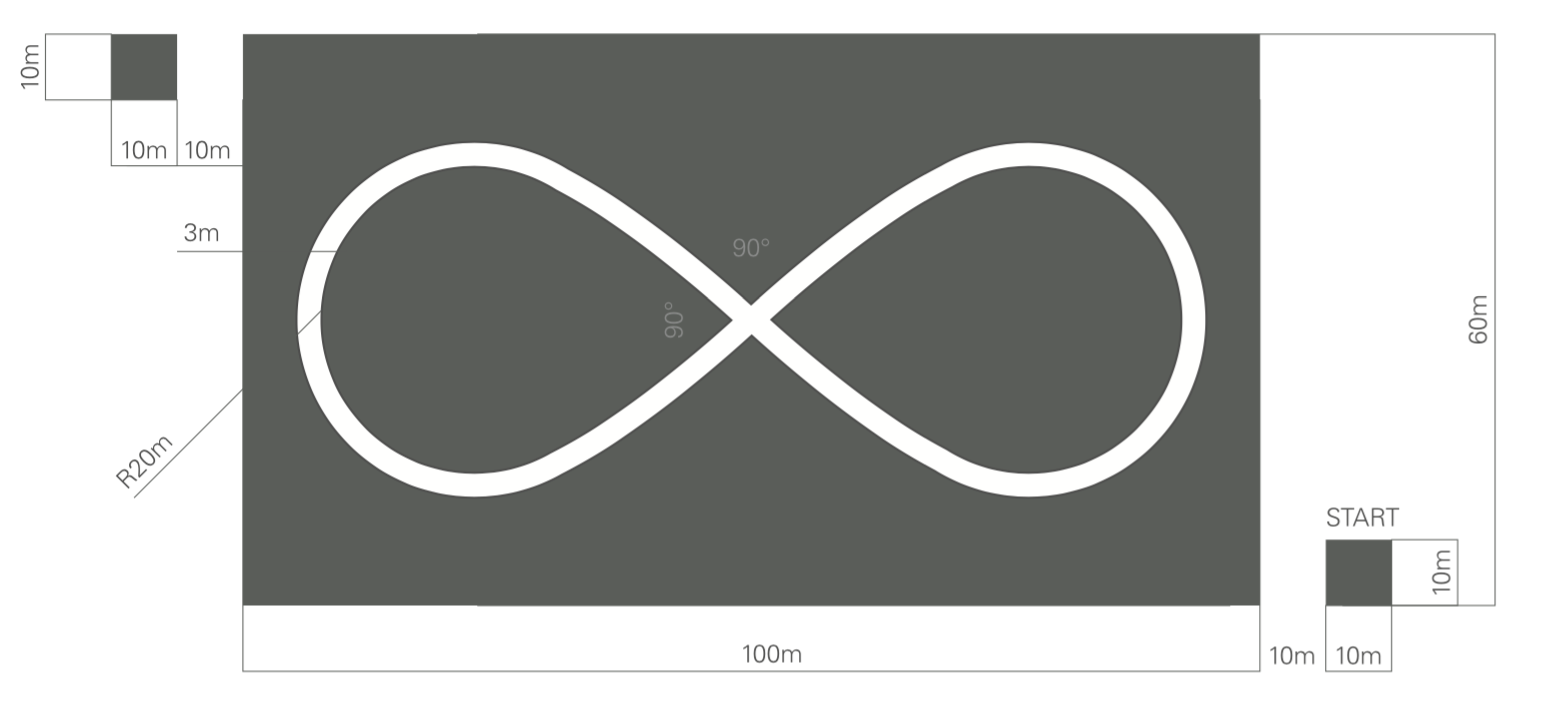
\includegraphics[width=1.1\textwidth]{img/arena.png}
    \caption{Arena of the challenge}
    \label{fig:arenachallenge}
\end{figure}

\subsection{Landing platform}
The landing platform is mounted on a ground vehicle of approximate dimensions $2.5m \times 1.5m \times 1.5m$ (length, width, height). The moving car starts at a constant speed of $15km/h$, it reduces the speed to $10km/h$ after 6 minutes and to $5 Km/h$ after 12 minutes.\\
The landing platform will be made of a ferrous surface to enable docking using magnetic or suction or other means.
It will be a square of dimensions $1.5m \times 1.5m$, and approximately $1.5m$ above ground, positioned on the vehicle. 
The landing zone inside the landing area is a circle of diameter $1m$. The center of the circle is indicated by an X. The landing area, the landing zone and the marker X are shown in Figure \ref{fig:finalplatform}.
A successful landing is when a point of contact of the UAV is within the landing circle, with propulsion off and rotors not spinning.

\begin{figure}[!htbp]
    \centering
    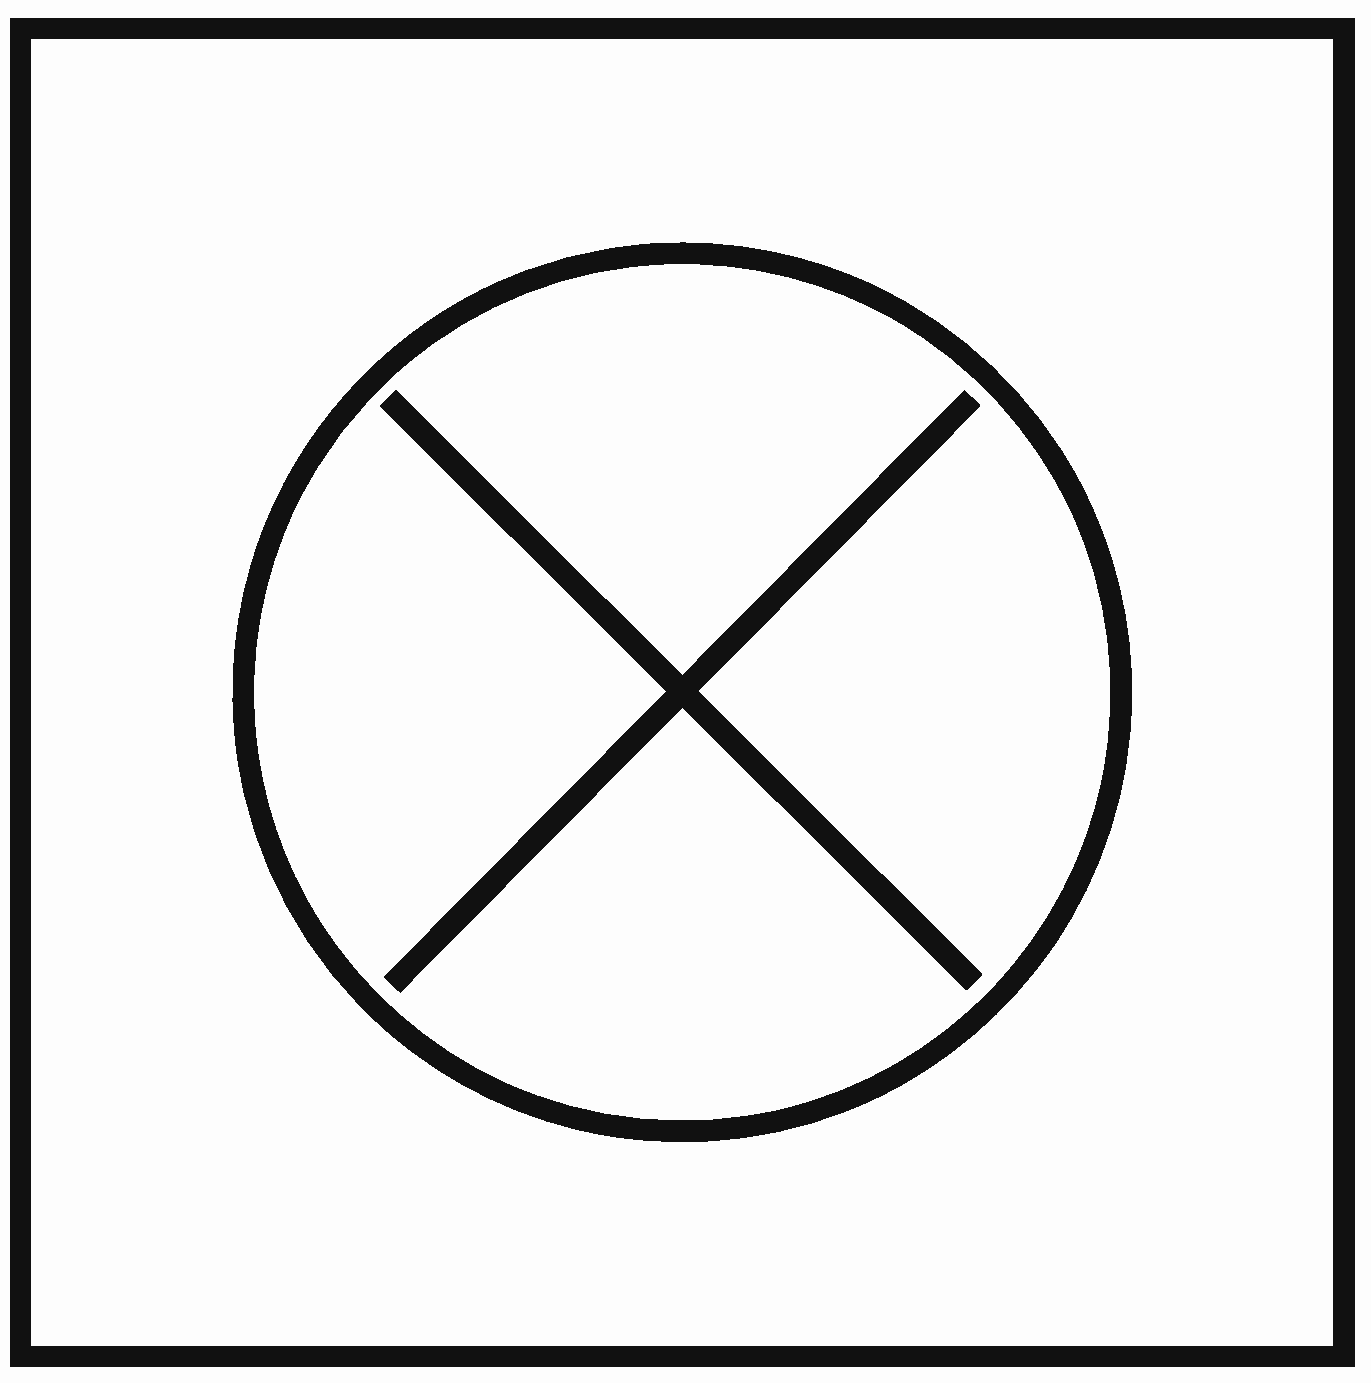
\includegraphics[width=0.5\textwidth]{img/base.pdf}
    \caption{Design of the platform in which the quadrotor must land on}
    \label{fig:finalplatform}
\end{figure}

\subsection{Infinity shape path}
The moving platform will move in an infinity-shape path described in the figure \ref{fig:arenachallenge}. 
We need to describe in a mathematical way this shape in order to use this information when we are estimating the state of the platform and to understand the right moment to perform the landing maneuver.\\
From the specification of the challenge:
\begin{itemize}
\item the car is moving with constant velocity $v_{tan}$ along the path
\item the radius of the circumferences that forms the trajectory is $r_{8}$m
\item the path is making a cross in the middle that creates 4 angles of $\frac{\pi}{2}$ 
\end{itemize}
The easiest way to describe this path is to define how the angle $\theta$ is changing in function of the space. \\
It easy to see that the shape can be seen as a combination of a cross and two circles.
The cross is simply defined as the union between the two line:
\begin{align}
\begin{split}
y &= x \\
y &= -x
\end{split}
\end{align}
while the two circles 
\begin{align}
\begin{split}
y^2 + (x - x_0)^2 &= r_{8}^2 \\
y^2 + (x + x_0)^2 &= r_{8}^2 
\end{split}
\end{align}
It easy to see that if we want the intersections between these two functions to be exactly in the 4 points we have to choose 
\begin{align}
\begin{split}
x_0 = \frac{\sqrt{2}}{2}r_{8}
\end{split}
\end{align}
That correspond to the 4 intersections coordinate
\begin{align}
\begin{split}
\Big(\frac{\sqrt{2}}{2}r_{8},\frac{\sqrt{2}}{2}r_{8}\Big);
\Big(\frac{\sqrt{2}}{2}r_{8},-\frac{\sqrt{2}}{2}r_{8}\Big);
\Big(-\frac{\sqrt{2}}{2}r_{8},-\frac{\sqrt{2}}{2}r_{8}\Big);
\Big(-\frac{\sqrt{2}}{2}r_{8},\frac{\sqrt{2}}{2}r_{8}\Big)
\end{split}
\end{align}

\begin{figure}[!htbp]
  \centering
 {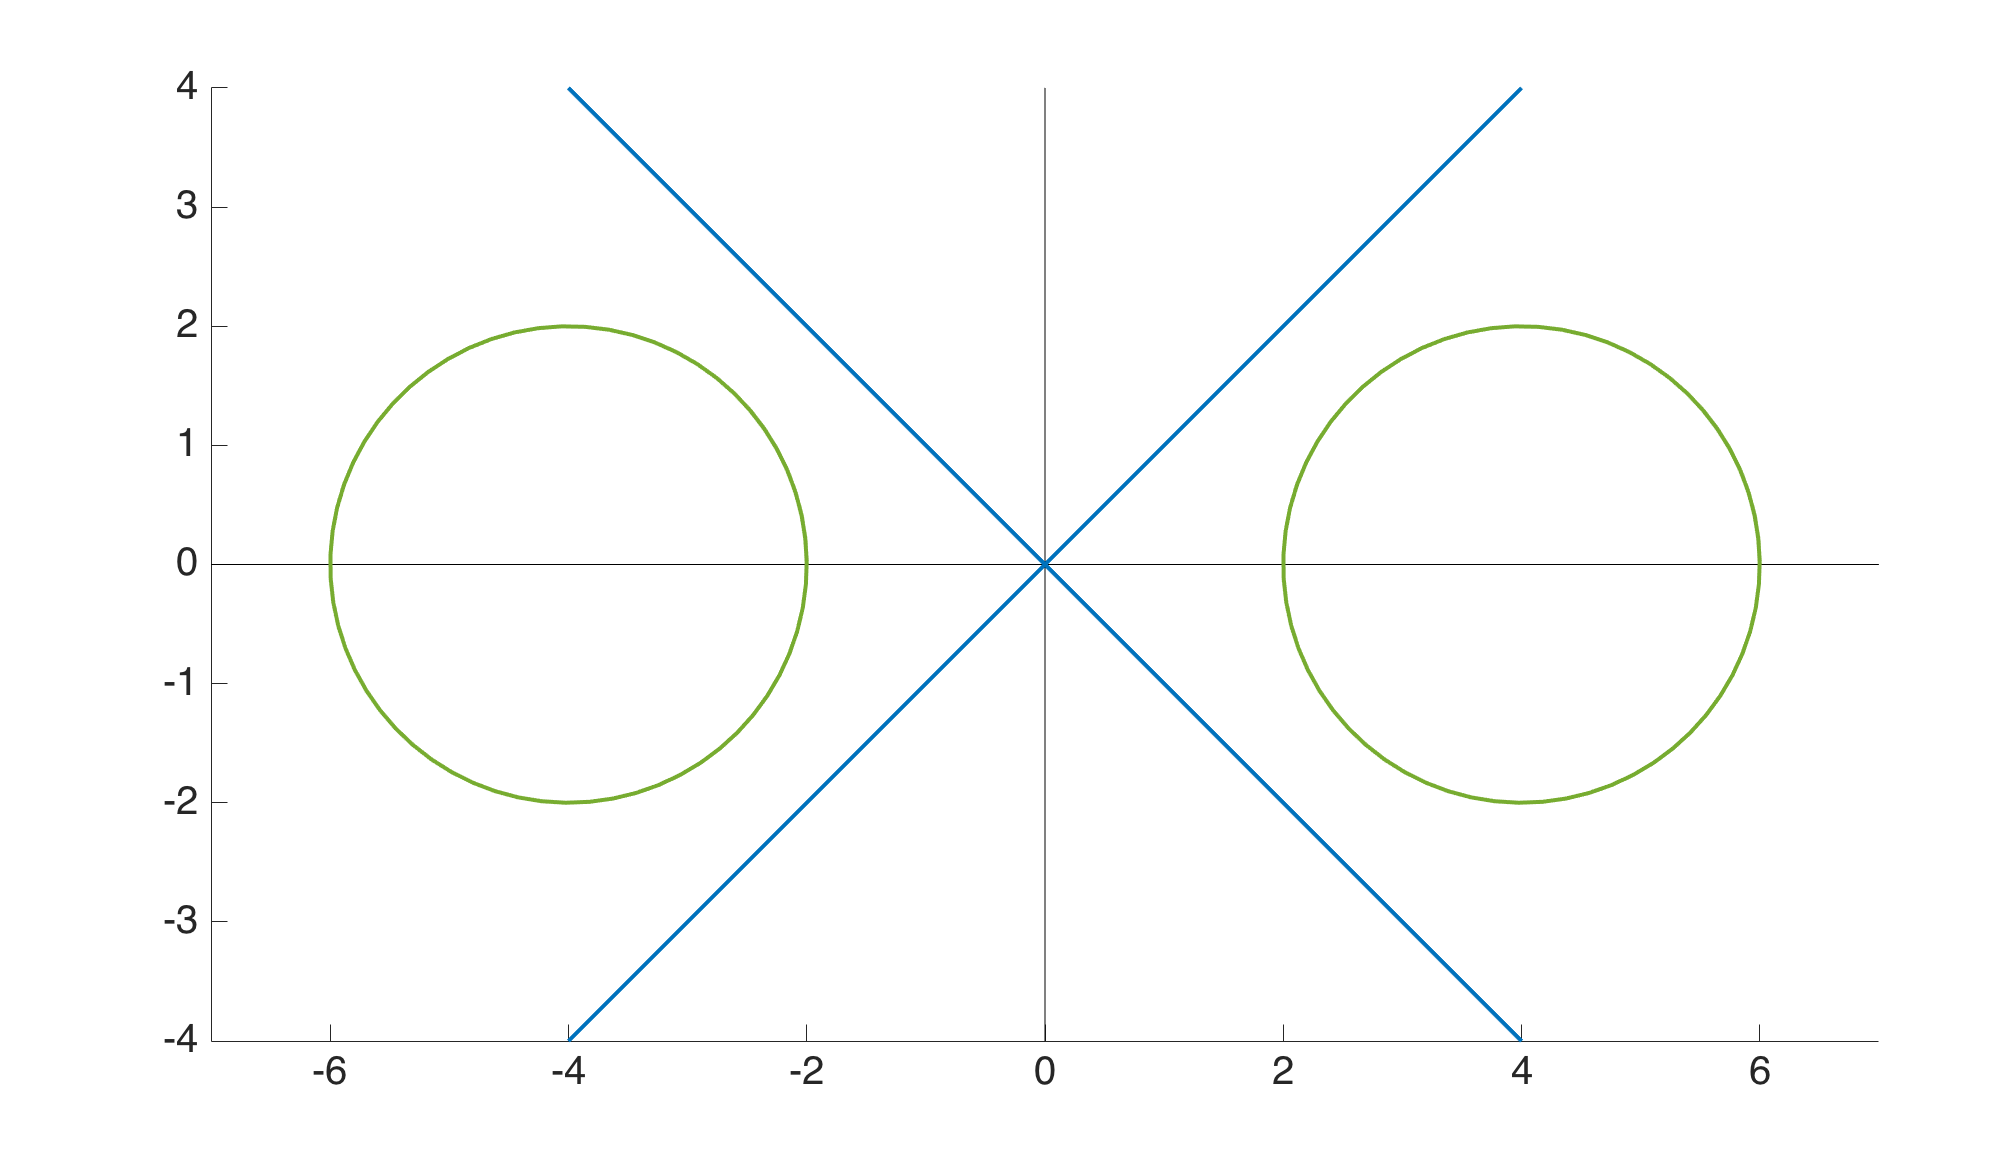
\includegraphics[width=0.48\textwidth]{img/constructionshape1_.png}\label{fig:constuctinfinity1}}
  \hfill
  {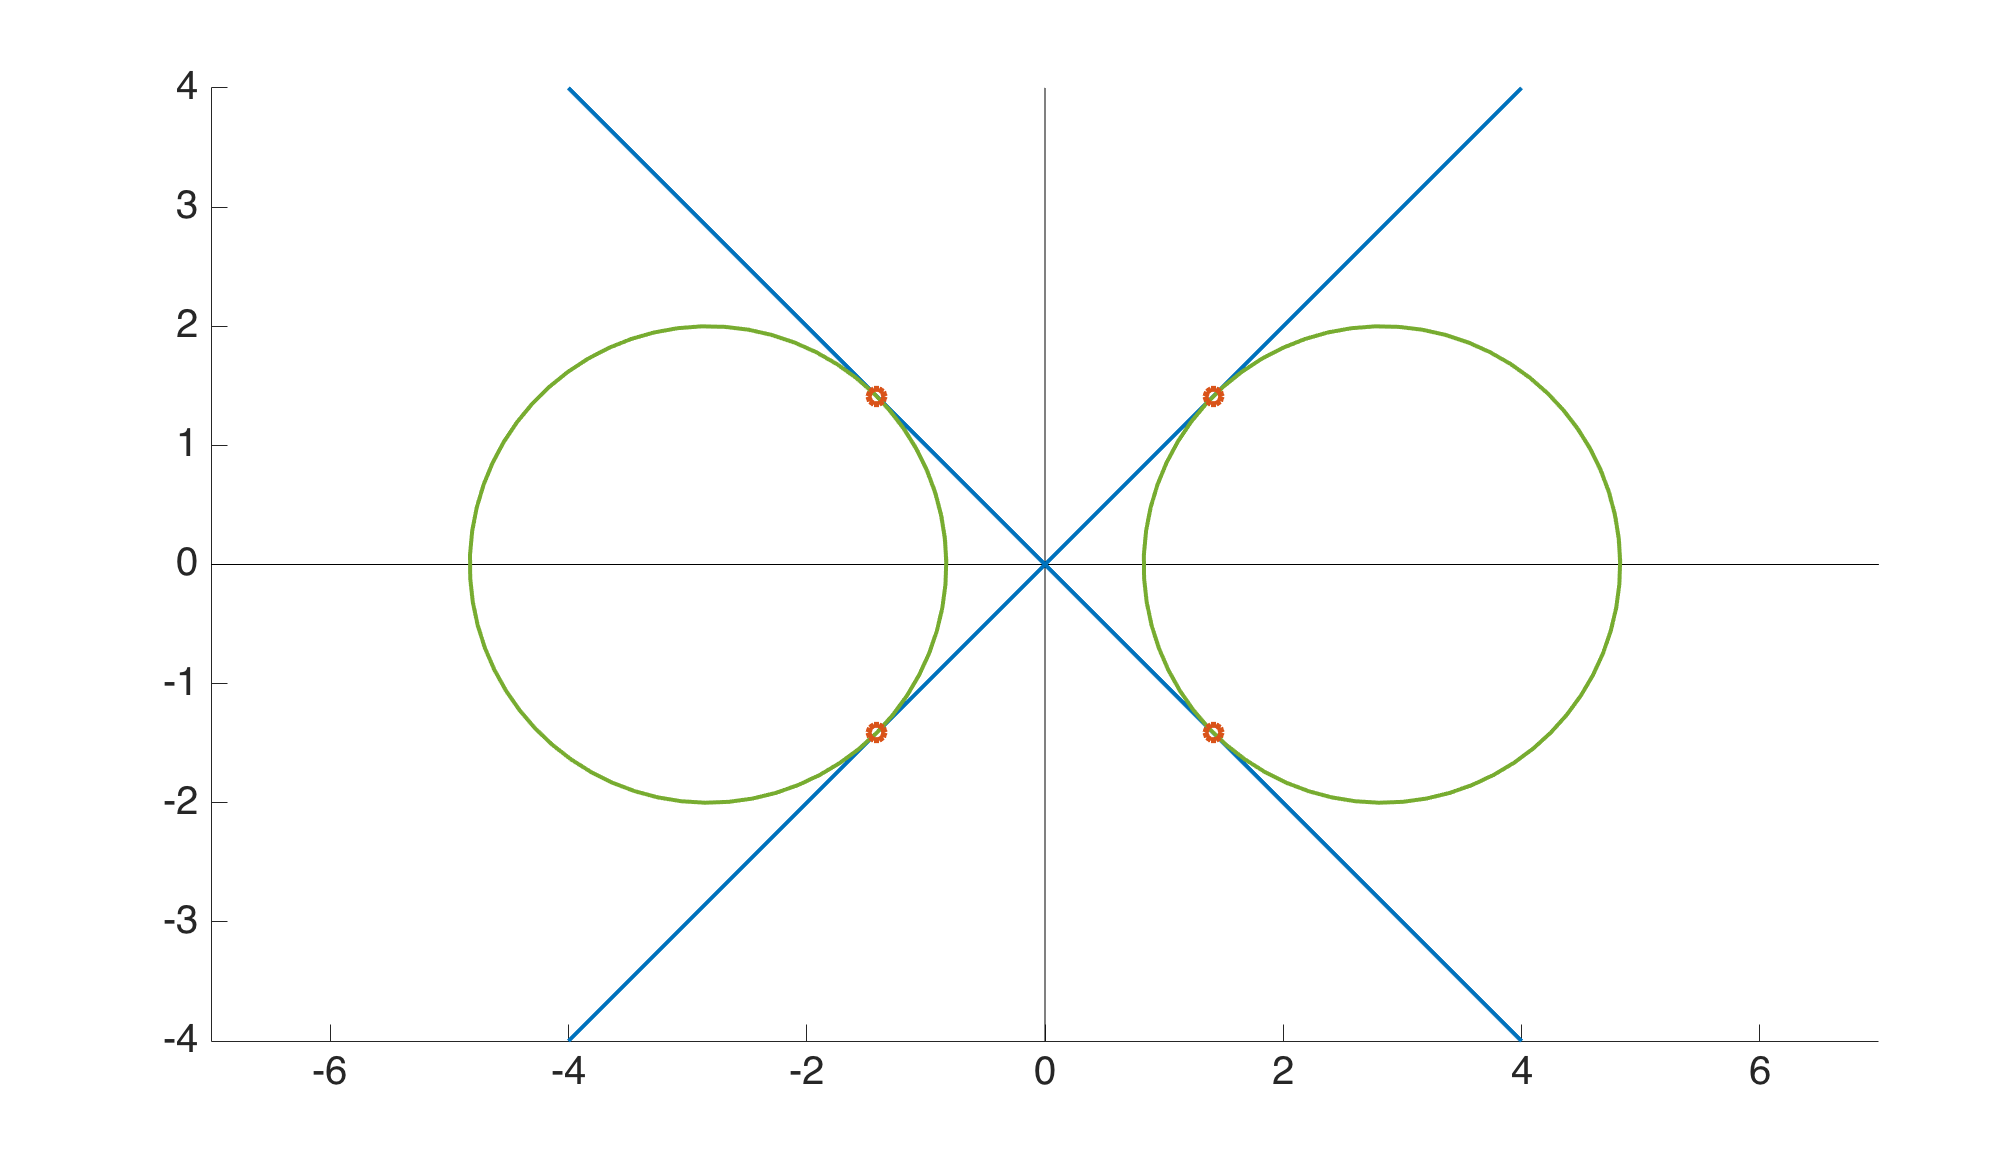
\includegraphics[width=0.48\textwidth]{img/constructionshape2_.png}\label{fig:constuctinfinity2}}
  \caption{How to construct the infinity-shape path}
\end{figure}

If we travel over the two circumferences the intersections correspond to angles $\theta = \pm \frac{3\pi}{4}$. \\
Now it is obvious to see that the path is symmetric and it can be divided in 4 parts and describing how the angle is changing in one of this section, the whole trajectory is defined.\\
We can observe that:
\begin{align}
\theta(x) =
\begin{cases}
    -\frac{x}{r_{8}}  &x\in \Big[0,\frac{3\pi}{4}r_{8}\Big] \quad \quad \ \ \  \\[10pt]
    -\frac{3\pi}{4} &x\in \Big[\frac{3\pi}{4}r_{8} ,\frac{3\pi}{4}r_{8} + r_{8}\Big]
\end{cases}
\end{align}
This function define a quarter of the trajectory \ref{fig:quarter_path} in function of the radius $r_{8}$ of the path.\\
It is now possible to use it to generate the entire trajectory $( x(t) , y(t) )$ \ref{fig:entire_path}: \\ we know that the length of the path is $$l = 4(\frac{3\pi}{4}r_{8} + r_{8})$$
and given the constant velocity $v_{tan}$ we can calculate the time to complete the trajectory 
$$T = \frac{l}{v_{tan}}$$
and it is simple to define $\theta(t)$ just stretching or shrinking $\theta(x)$ .\\
So we can now define:
\begin{align}
\begin{split}
\dot{x} &= v_{tan} cos(\theta(t)) \\
\dot{y} &= v_{tan} sin(\theta(t))
\end{split}
\end{align}
And finally we also need the discretized verison obtain just by forward Euler approximation:
\begin{align}
\begin{split}
x_k &= x_{k-1} + dt \big(v_{tan k-1} cos(\theta_{k-1})\big) \\
y_k &= y_{k-1} + dt \big(v_{tan k-1} sin(\theta_{k-1})\big)
\end{split}
\end{align}

\begin{figure}[!htbp]
  \centering
 {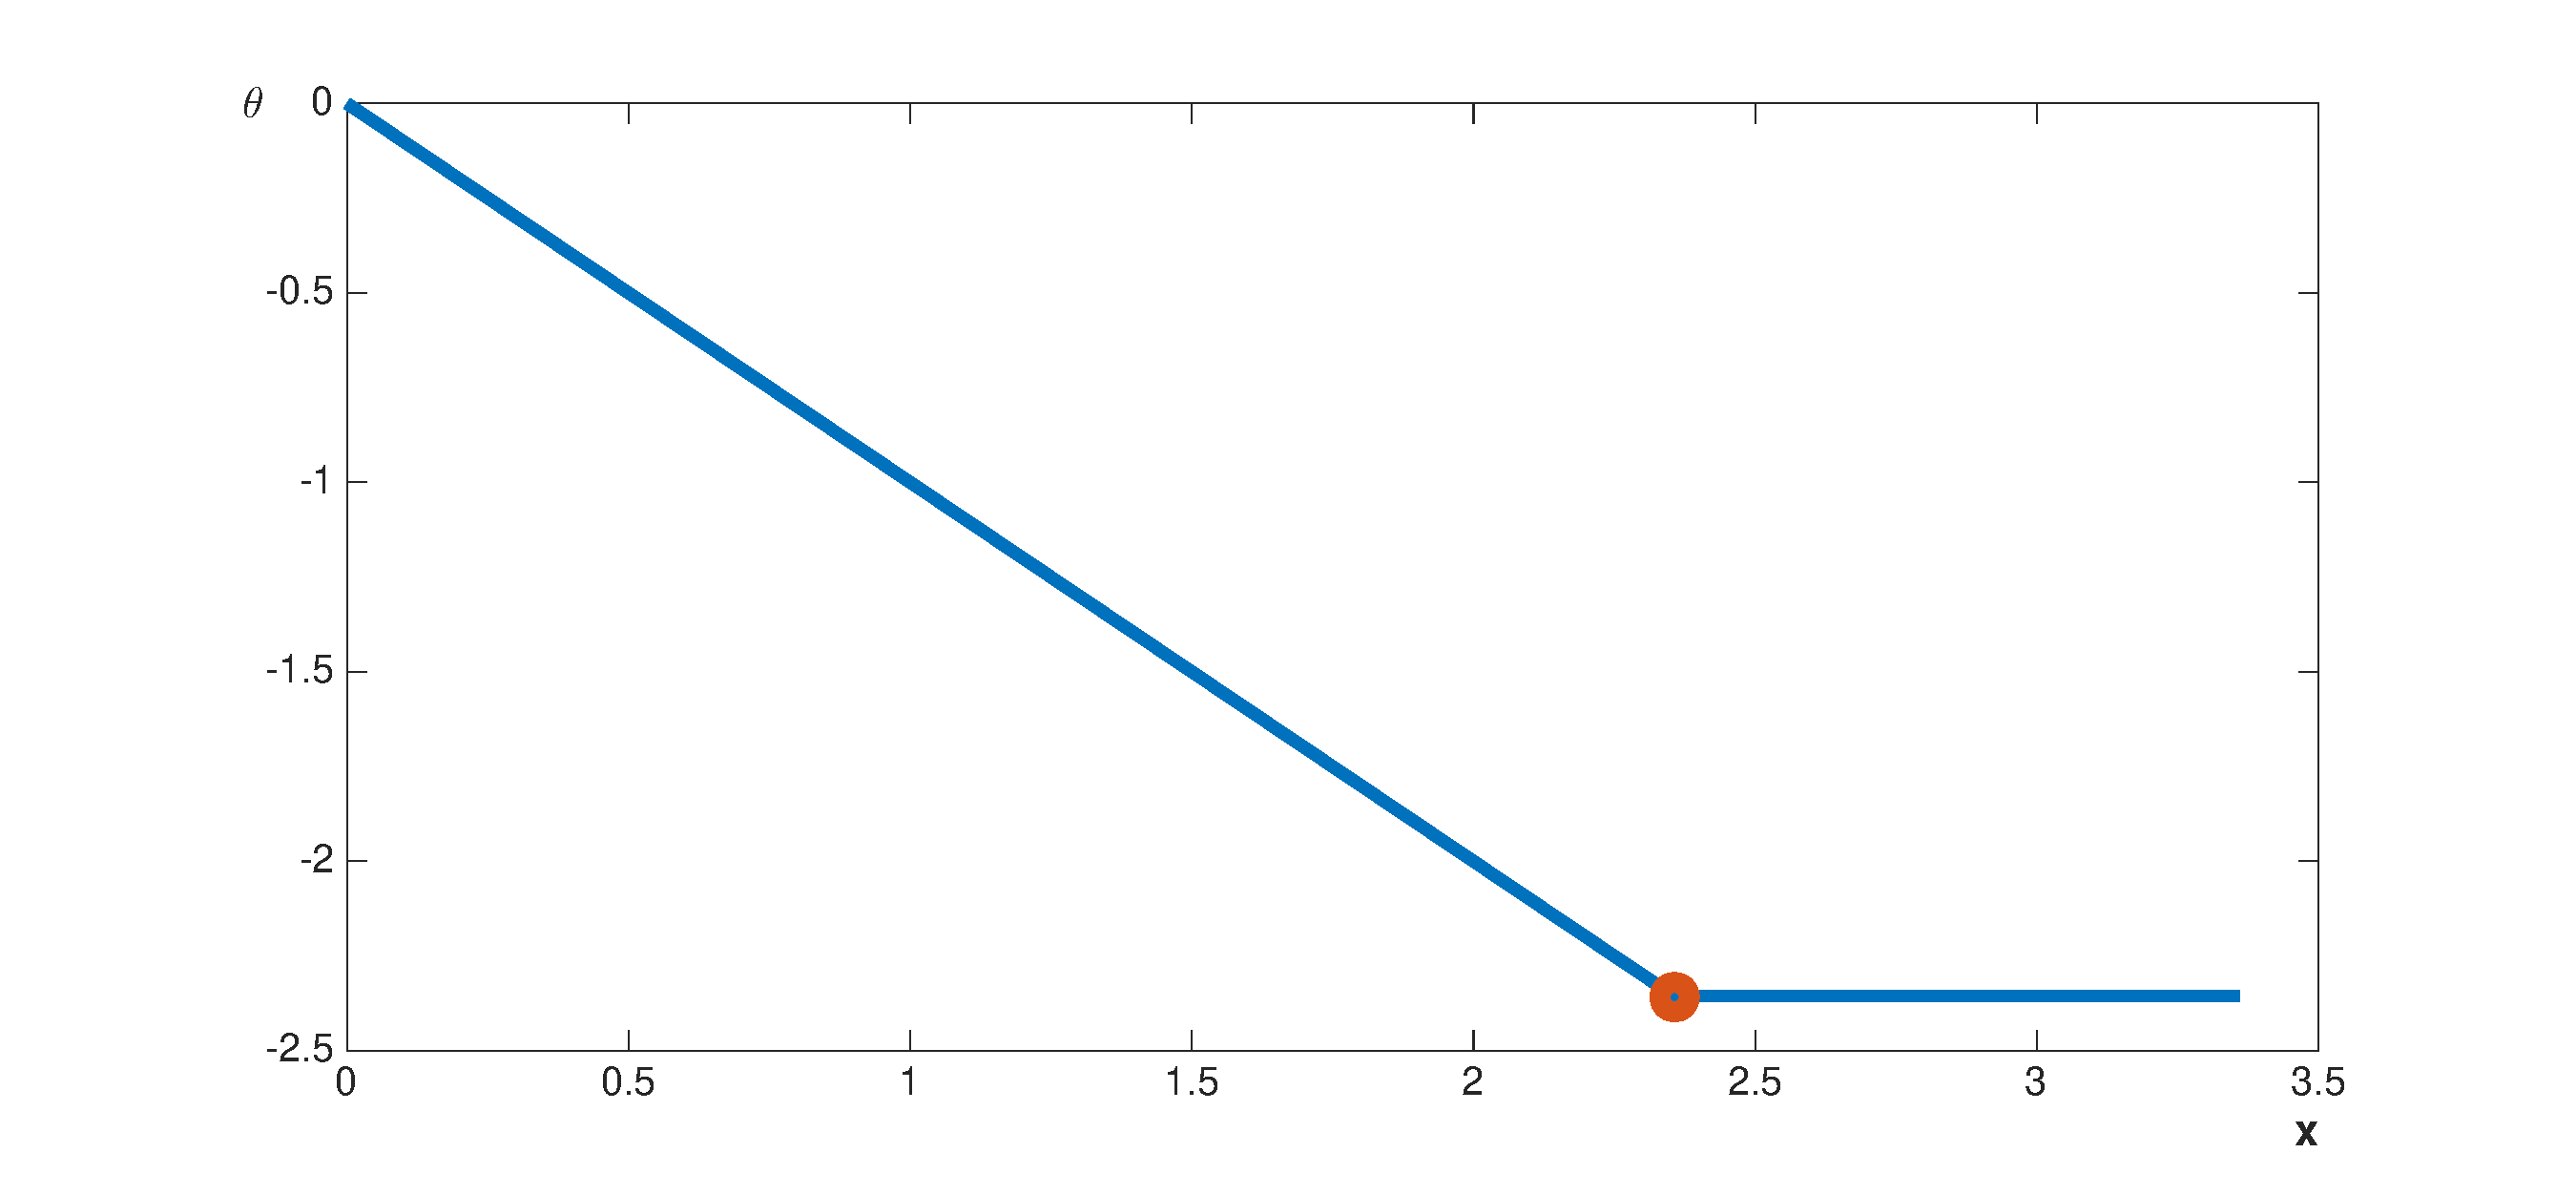
\includegraphics[width=0.8\textwidth]{img/angle_x.eps}\label{fig:quarter_theta}}
  \hfill
  {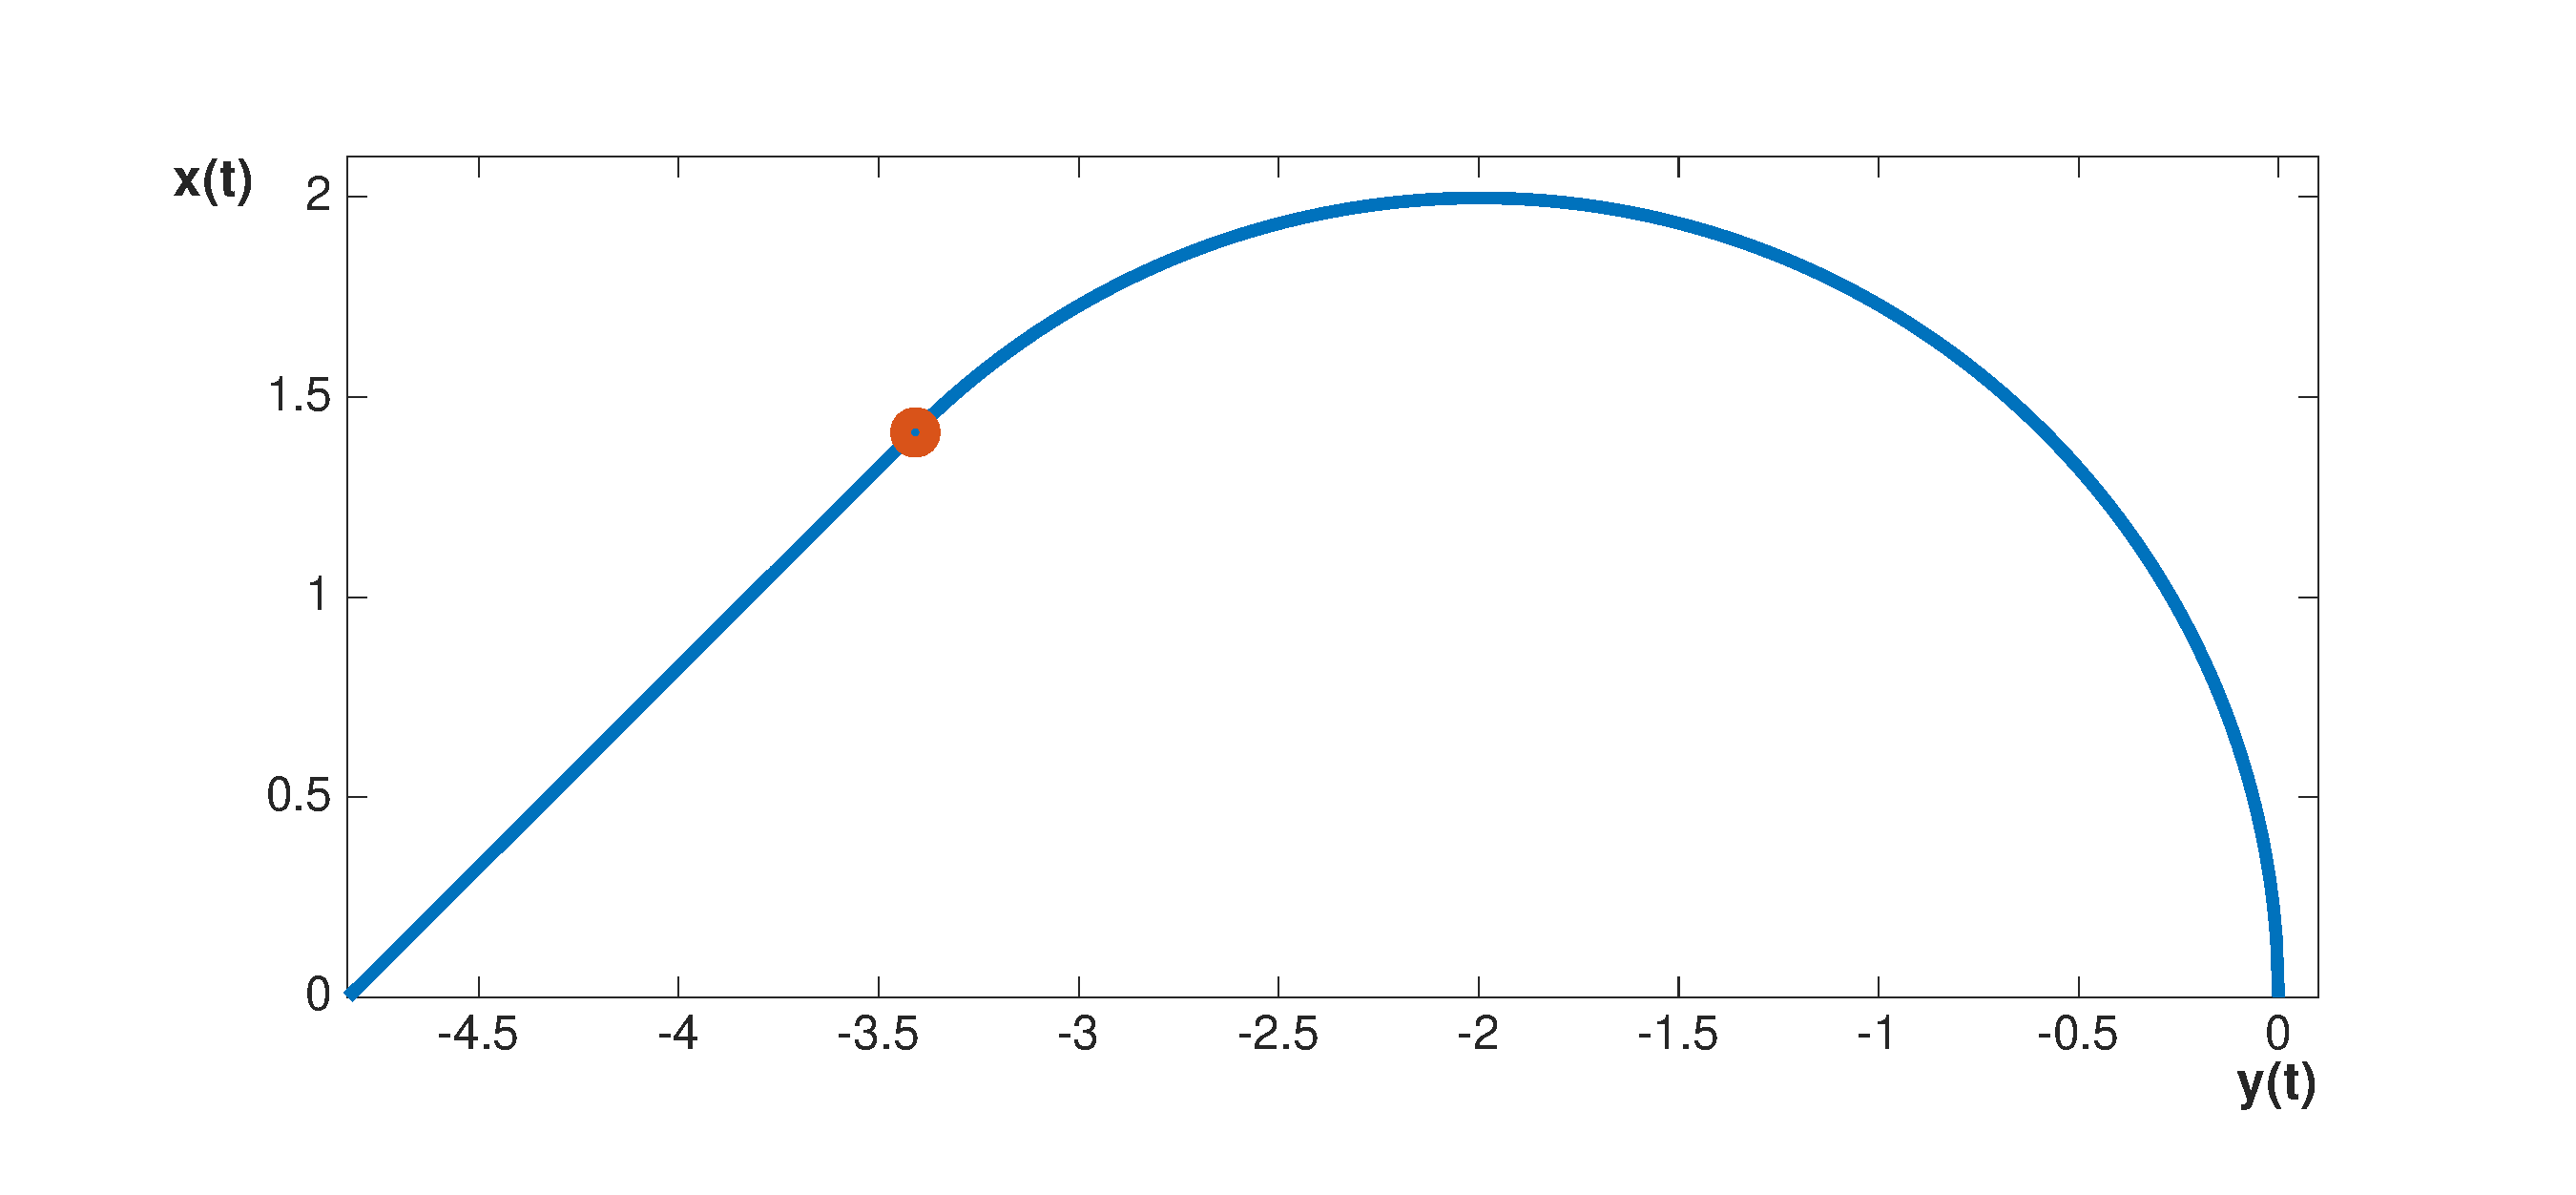
\includegraphics[width=0.8\textwidth]{img/path_x_quarter.eps}\label{fig:quarter_xy}}
  \caption{The parametrization of a quarter of the path}
  \label{fig:quarter_path}
\end{figure}

\begin{figure}[!htbp]
    \centering
    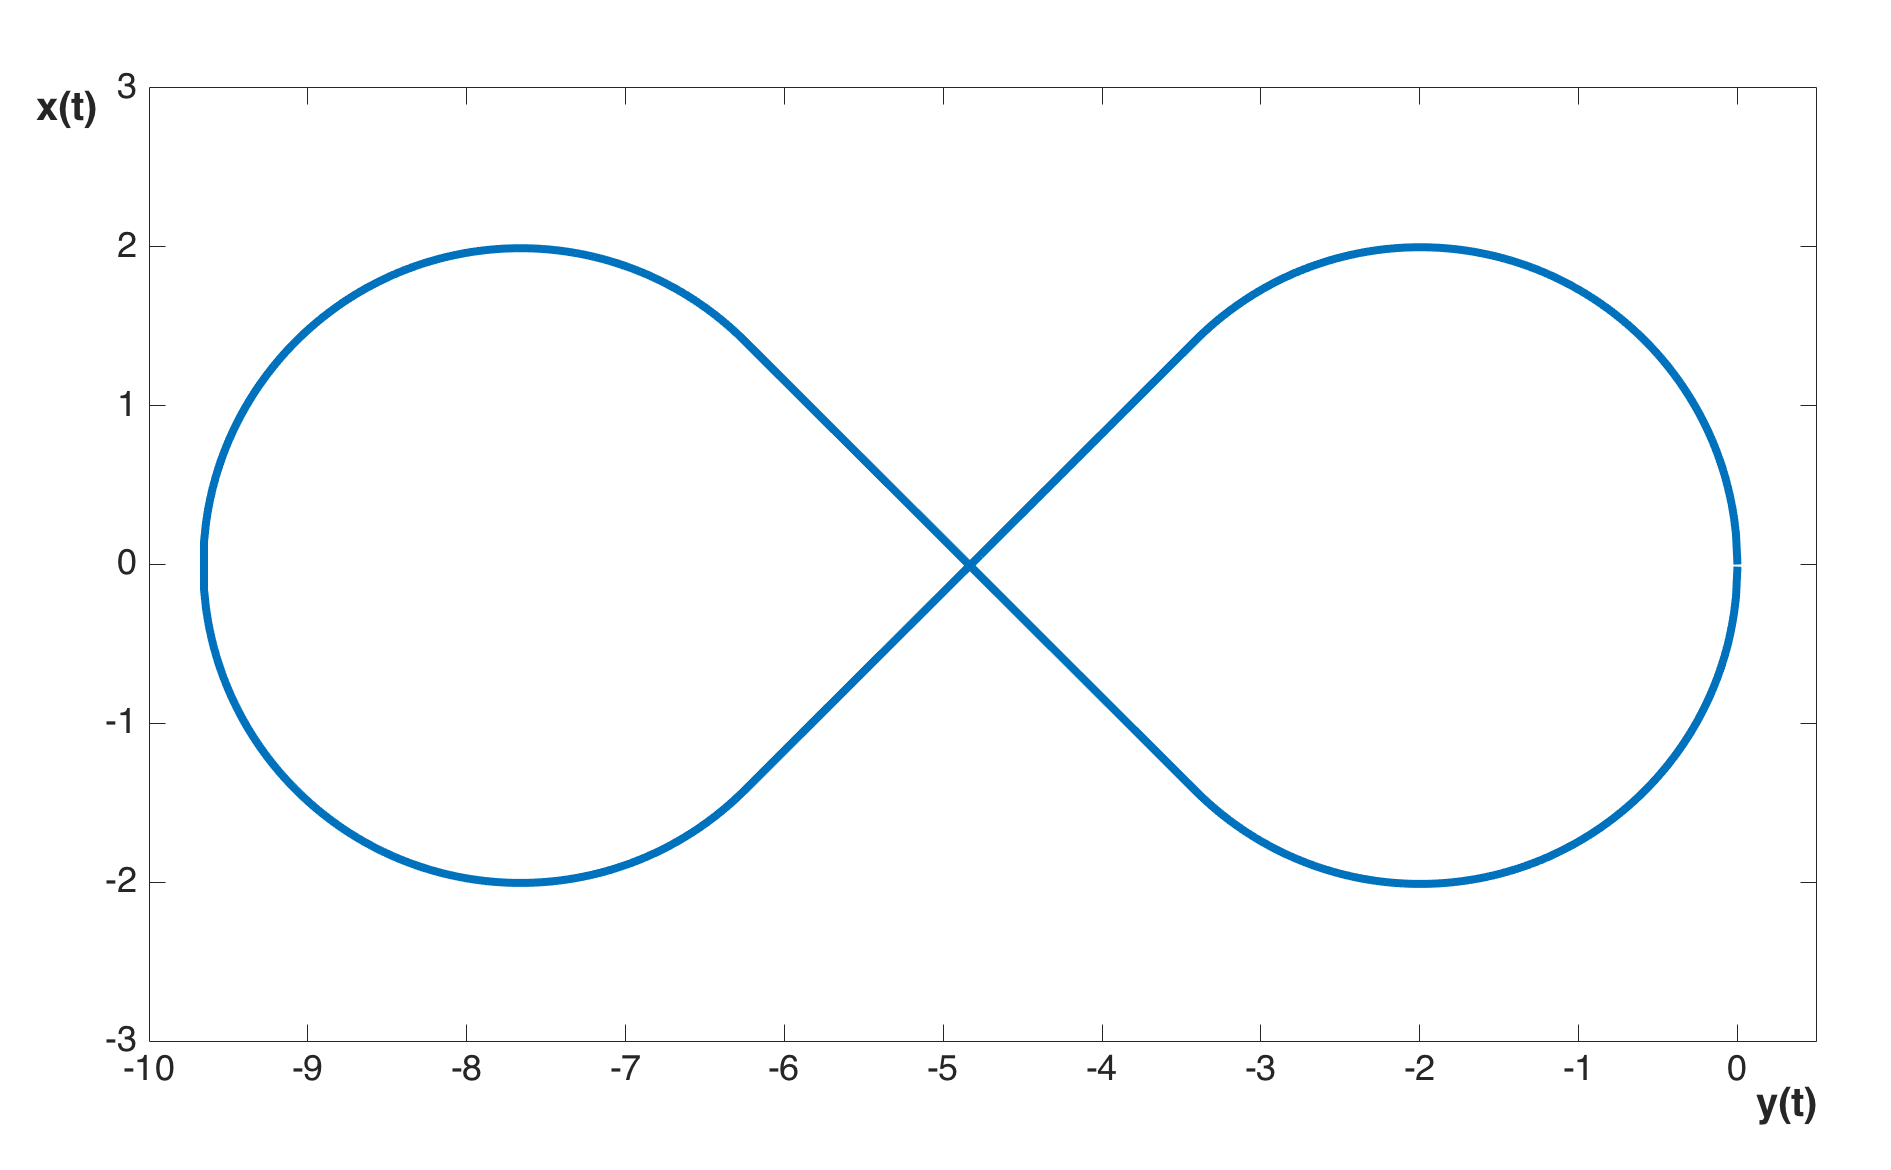
\includegraphics[width=1\textwidth]{img/infinityshapepath.png}
    \caption{Infinity-shape path}
    \label{fig:entire_path}
\end{figure}

\section{Simulation}


\chapter{General Framework}\label{chap:general_framework}
Our framework consists in several parts, each one is computing a different sub-task and they are communicating one with the other in order to achieve the final mission of landing on a moving platform. Figure \ref{fig:pipeline_diagram} shows the principal components of our framework. In this chapter we are giving a brief introduction on each part and in the following chapters we will discuss in detail the parts developed in this thesis.
\begin{figure}[!ht]
    \centering
    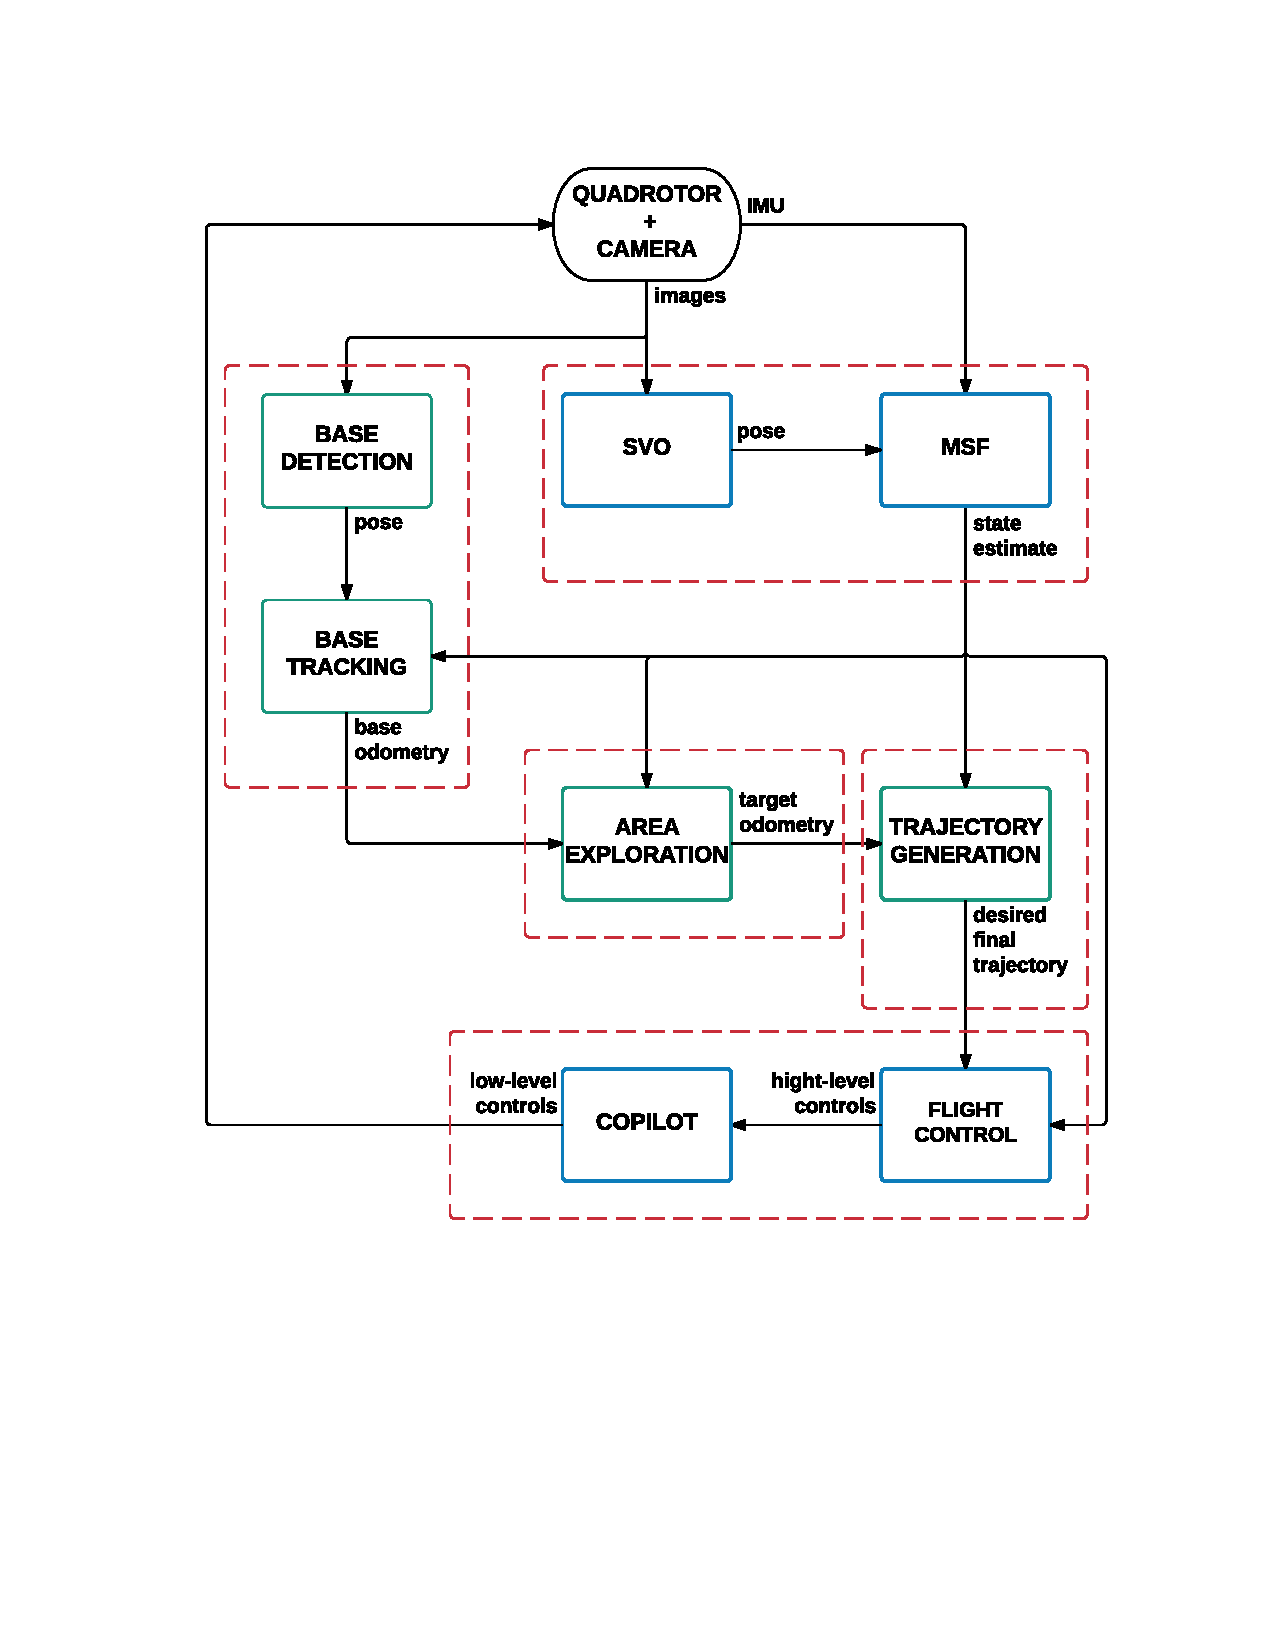
\includegraphics[width=1.0\textwidth]{img/pipeline_diagram.pdf}
    \caption{Pipeline of the framework. In blue the modules already implemented we add to the work of this thesis. In green the steps developed in this work.}
    \label{fig:pipeline_diagram}
\end{figure}

The modular system developed, utilize the Robot Operating System (ROS) \cite{ros} for interprocess communication. The platforms used in this project are capable of autonomous, vision-based flight utilizing only their on-board hardware resources, they do not need to rely on external communication infrastructure to accomplish their tasks. In a field robotics scenario with uncertain communication reliability like the MBZIRC, this is of critical importance, and our approach enables our platforms to perform their missions
autonomously without any dependence on external communication.

\section{SVO \& MSF} \label{sec:state_estimation}
The backbone of our system is an accurate state estimation provided by the visual odometry algorithm: Semidirect Monocular Visual Odometry (SVO) \cite{forster2014svo}. It provides a precise and robust pose estimate (3D positiona and orientation), and it runs at up to 55 frames per second on the onboard embedded computer of our flying robots. This vision-based state estimate is fused with inertial data and gravity aligned using the Multi-Sensor Fusion framework (MSF) \cite{lynen2013robust}.\\
The fusion of visual and inertial information provides a full state estimate of the UAVs.\\


\subsection{SVO}

SVO implements a semi-direct monocular visual odometry algorithm that estimates the motion of a camera in real time using sequential images. It combines the advantages of features extraction methods and direct approaches.\\
The standard techniques consist in the extraction of a sparse set of features in each image, match them in successive frames using invariant feature descriptors, reconstruct camera motion and structure using epipolar geometry and finally, refine the pose and structure through reprojection error minimization. \\
On the other hand appearance-based, or direct, methods estimate structure and motion directly from intensity values of the image: the camera pose relative to the previous frame is found through minimizing the photometric error between pixels.\\

%The majority of VO algorithms [12] follows this procedure, independent of the applied optimization framework. A reason for the success of these methods is the availability of robust feature detectors and descriptors that allow matching between images even at large inter-frame movement. The disadvantage of feature-based approaches is the reliance on detection and matching thresholds, the neccessity for robust estimation techniques to deal with wrong correspondences, and the fact that most feature detectors are optimized for speed rather than precision, such that drift in the motion estimate must be compensated by averaging over many feature-measurements.

%Direct methods that exploit all the information in the image, even from areas where gradients are small, have been shown to outperform feature-based methods in terms of robustness in scenes with little texture [14] or in the case of camera- defocus and motion blur [15]. The computation of the photometric error is more intensive than the reprojection error, as it involves warping and integrating large image regions. However, since direct methods operate directly on the intensitiy values of the image, the time for feature detection and invariant descriptor computation can be saved.


The semi-direct approach computes an initial guess of the relative camera motion and the feature correspondences using direct methods and concludes with a feature-based nonlinear reprojection-error refinement. This technique increases the computational speed due to the lack of feature-extraction at every frame (this operation is only required when a key-frame is selected to initialize new 3D points), furthermore it increases robustness and precision using many small patches (instead of few large planar patches).
A new 3D point is insert in the set used for motion estimation when its depth uncertainty becomes small enough. To estimate it, a probabilistic depth-filter is initialized for each 2D feature for which the corresponding 3D point is to be estimated, the filters are initialized with a large uncertainty in depth and at every subsequent frame it is updated in a Bayesian fashion.

%The proposed sparse model-based image alignment algorithm for motion estimation is related to model-based dense image alignmen.. However, we demonstrate that sparse information of depth is sufficient to get a rough estimate of the motion and to find feature- correspondences. As soon as feature correspondences and an initial estimate of the camera pose are established, the algorithm continues using only point-features; hence, the name “semi-direct”. This switch allows us to rely on fast and established frameworks for bundle adjustment.
%A Bayesian filter that explicitly models outlier measurements is used to estimate the depth at feature locations. A 3D point is only inserted in the map when the corresponding depth-filter has converged, which requires multiple measurements. The result is a map with few outliers and points that can be tracked reliably.

%eliminates the need of costly feature extraction and robust matching techniques for motion estimation. The algorithm operates directly on pixel intensities, which results in subpixel precision at high frame-rates.

%A probabilistic mapping method that explicitly models outlier measurements is used to estimate 3D points, which results in fewer outliers and more reliable points.

%Precise and high frame-rate motion estimation brings increased robustness in scenes of little, repetitive, and high-frequency texture.

\subsection{MSF}
MSF implements an Iterated Extended Kalman Filter (IEKF) \cite{bell1993iterated} over variable sized windows of updates. In the IEKF  the state prediction is driven by IMU data, while the update step can be of any nature, in our case we use the pose given by SVO.\\
MSF has a modular structure that can support and marge an unlimited number of sensors that give relative or absolute measurements (pose, position, pressure, etc). Furthermore it estimates the calibration states between sensors and tracks the cross covariance terms for relative updates. It also has an outlier rejection module for the update measures.\\
MSF can compensate for unknown and changing delays implementing further propagation: the state is predicted with IMU data and whenever it receives an update step (usually in the past because of delays) it collocates this measurement in a ring-buffer that considers the moment this data was taken. Then it propagates this measure in time in order to update the current estimation and covariance based on the past data. With this function the framework can give state estimation at IMU rate and without delay.


\section{High \& low level controls}
To control the flight of the quadrotor we need an algorithm that given the current state of the UAV and a final desired state it calculate the input that bring and stabilize the quad on the desired final condition.\\
The controller of the quadrotor is split into a high-level part and a low-level part: the former enables the tracking of a desired  pose and velocity and gives the input to the letter that tracks a desired thrust and body rates.\\

\subsection{High part}\label{sec:high_control}

The high level control takes as input: 
\begin{itemize}
\item $([\hat{x},\hat{y},\hat{z}],[\hat{\phi},\hat{\theta},\hat{\psi}],[\hat{vx},\hat{vy},\hat{vz}],[\hat{p},\hat{q},\hat{r}])$: the current state estimate (position, orientation, velocity, angular velocity) , calculate in the previous module
\item $([x_{ref},y_{ref},z_{ref}],[vx_{ref},vy_{ref},vz_{ref}],[ax_{ref},ay_{ref},az_{ref}],[\psi_{ref}])$: a reference state (position, velocity, acceleration, yaw) , that can be sampled from a trajectory, calculate in another module, that the UAV should track to perform a task
\end{itemize}
and gives in output:
\begin{itemize}
\item $c_{des}$: the desired normalize thrust 
%\item $(\phi_{des},\theta_{des},\psi_{des})$: the desired attitude or
\item $(p_{des},q_{des},r_{des})$: the desired body rates
\end{itemize}
which are sent to the low-level controller.\\

The high level controller is composed by a position controller followed by an attitude controller, synchronized at 50Hz.

\subsubsection{Position Controller}
PD controller with feedback terms on the reference position and velocity and feedfoward on the reference acceleration:
\begin{align}
\begin{bmatrix}
ax_{des}  \\[10pt]
ay_{des}  \\[10pt]
az_{des}
\end{bmatrix} = P_{pos}
\begin{bmatrix}
x_{ref} - \hat{x} \\[10pt]
y_{ref} - \hat{y}  \\[10pt]
z_{ref} - \hat{z}
\end{bmatrix} + 
D_{pos}
\begin{bmatrix}
vx_{ref} - \hat{vx} \\[10pt]
vy_{ref} - \hat{vy}  \\[10pt]
vz_{ref} - \hat{vz}
\end{bmatrix}
+
\begin{bmatrix}
ax_{ref} - \hat{0} \\[10pt]
ay_{ref} - \hat{0}  \\[10pt]
az_{ref} - \hat{g}
\end{bmatrix}
\label{eq:PDcontroller1}
\end{align}

Where $P_{pos} = diag(p_{xy} ,p_{xy} ,p_{z} )$ and $D_{pos} = diag(d_{xy} ,d_{xy} ,d_{z} )$ are gain matrices.

%\begin{align}
%\begin{bmatrix}
%ax_{des}  \\[10pt]
%ay_{des}  \\[10pt]
%az_{des}
%\end{bmatrix}
%= 
%\begin{bmatrix}
%p_{xy} (x_{ref} - \hat{x}) + d_{xy}(vx_{ref} - \hat{vx}) + ax_{ref}  \\[10pt]
%p_{xy} (y_{ref} - \hat{y}) + d_{xy}(vy-{ref} - \hat{vy}) + ay_{ref}  \\[10pt]
%p_{z} (z_{ref} - \hat{z}) + d_{z}(vz_{ref} - \hat{vz}) + az_{ref} - g 
%\end{bmatrix}
%\label{eq:PDcontroller2}
%\end{align}
Now is very simple to derived the desired normalized thrust  $c_{des}$: it is the projection of  $a_{des}$  on the current $z$ axes of the UAV:
\begin{align}
c_{des} = a_{des} \cdot e_z^B
\label{eq:thrust}
\end{align}

\subsubsection{Attitude Controller}
The output of this controller is $a_{des}$ and together with $\psi_{ref}$ encoded the desired orientation:
Since the quadrotor can only accelerate in direction of the z direction of the body we want to align this axis  with the desired acceleration $a_{des}$, so it enforce both $\phi_{des}$ and $\theta_{des}$. The third degree of freedom is given by $\psi_{ref}$.\\
With some geometric calculations it easy to define $(p_{des},q_{des},r_{des})$: these values are just function of the current orientation $(\hat{\phi},\hat{\theta},\hat{\psi})$, the desired final orientation of the z axis $e_{z,des}^B = \frac{ a_{des}}{|| a_{des}||}$ and the desired final yaw $\psi_{des} = \psi_{ref}$. \\


TODO calculations??\\


%To calculate $p_{des}$ and $q_{des}$ the following calculations are computed:
%\begin{align}
%\begin{split}
%e_{z,des}^B = \frac{ a_{des}}{|| a_{des}||} \\[10pt]
%\alpha = \cos^{-1}{e_{z}^B \cdot e_{z,des}^B} \\[10pt]
%\boldsymbol{n} = \frac{e_{z}^B times e_{z,des}^B}{||e_{z}^B times e_{z,des}^B||}
%\end{split}
%\label{eq:thrust}
%\end{align}
%where $e_{z,des}^B$ is the desired orientation of the z axis, $\alpha$ is the error angle and $\boldsymbol{n} $ is the rotation axis

\subsection{Low part}
The low level control takes as input:
 \begin{itemize}
\item $c_{des}$: the desired normalize thrust 
\item $(p_{des},q_{des},r_{des})$: the desired body rates
\item $(\hat{p},\hat{q},\hat{r})$: the current estimate angular velocity
\end{itemize}
and gives in output:
\begin{itemize}
\item $(f_{1,des},f_{2,des},f_{3,des},f_{4,des})$: the desired nominal rotor thrusts.
\end{itemize}

We can compute the desired torques $\boldsymbol{\tau}_{des}$ with the feedback linerized scheme:
\begin{align}
\begin{bmatrix}
\tau p_{des}  \\[10pt]
\tau q_{des}  \\[10pt]
\tau r_{des}
\end{bmatrix} 
= JP_{att}
\begin{bmatrix}
p_{des} - \hat{q} \\[10pt]
q_{des} - \hat{q}  \\[10pt]
r_{des} - \hat{r}
\end{bmatrix} + 
\begin{bmatrix}
\hat{q} \\[10pt]
\hat{q}  \\[10pt]
\hat{r}
\end{bmatrix}
\times
J
\begin{bmatrix}
\hat{q} \\[10pt]
\hat{q} \\[10pt]
\hat{r}
\end{bmatrix}
\label{eq:torques}
\end{align}
Where $P_{att} = diag(p_{qp} ,p_{qp} ,p_{r} )$ is a gain matrix and  $J = diag(J_{xx} ,J_{yy} ,J_{zz} )$ is the inertia matrix for rotation around the center of mass.\\
Now to find the thrusts for each rotor we have to solve:
\begin{align}
\begin{bmatrix}
f_{1,des}  \\[10pt]
f_{2,des}  \\[10pt]
f_{3,des}  \\[10pt]
f_{4,des}  
\end{bmatrix} 
=
\begin{bmatrix}
\frac{1}{4\lambda_1} \big(m c_{des} + \frac{\tau r_{des}}{\kappa} - \frac{\sqrt{2}\tau q_{des}}{l} + \frac{\sqrt{2}\tau p_{des}}{l}\big) \\[10pt]
\frac{1}{4\lambda_2} \big(m c_{des} - \frac{\tau r_{des}}{\kappa} - \frac{\sqrt{2}\tau q_{des}}{l} - \frac{\sqrt{2}\tau p_{des}}{l}\big) \\[10pt]
\frac{1}{4\lambda_3} \big(m c_{des} + \frac{\tau r_{des}}{\kappa} + \frac{\sqrt{2}\tau q_{des}}{l} - \frac{\sqrt{2}\tau p_{des}}{l}\big)\\[10pt]
\frac{1}{4\lambda_4} \big(m c_{des} - \frac{\tau r_{des}}{\kappa} + \frac{\sqrt{2}\tau q_{des}}{l} + \frac{\sqrt{2}\tau p_{des}}{l}\big)
\end{bmatrix} 
\label{eq:thrusts}
\end{align}
where $\kappa$ is the rotor-torque coefficient and $\lambda_i$ are the rotor fitness coefficients, $l$ is the arm length between the center of mass and the point in which the thrust is applied (all of them are parameters of the quadrotor). \\
Depending on the chosen orientation of the body frame we have a different map between torques $\tau i_{des}$ and thrusts $f_j$, in our case the figure \ref{fig:bodyframe} shows how our coordinate system is oriented w.r.t the 4 propellers.

\begin{figure}[!ht]
    \centering
    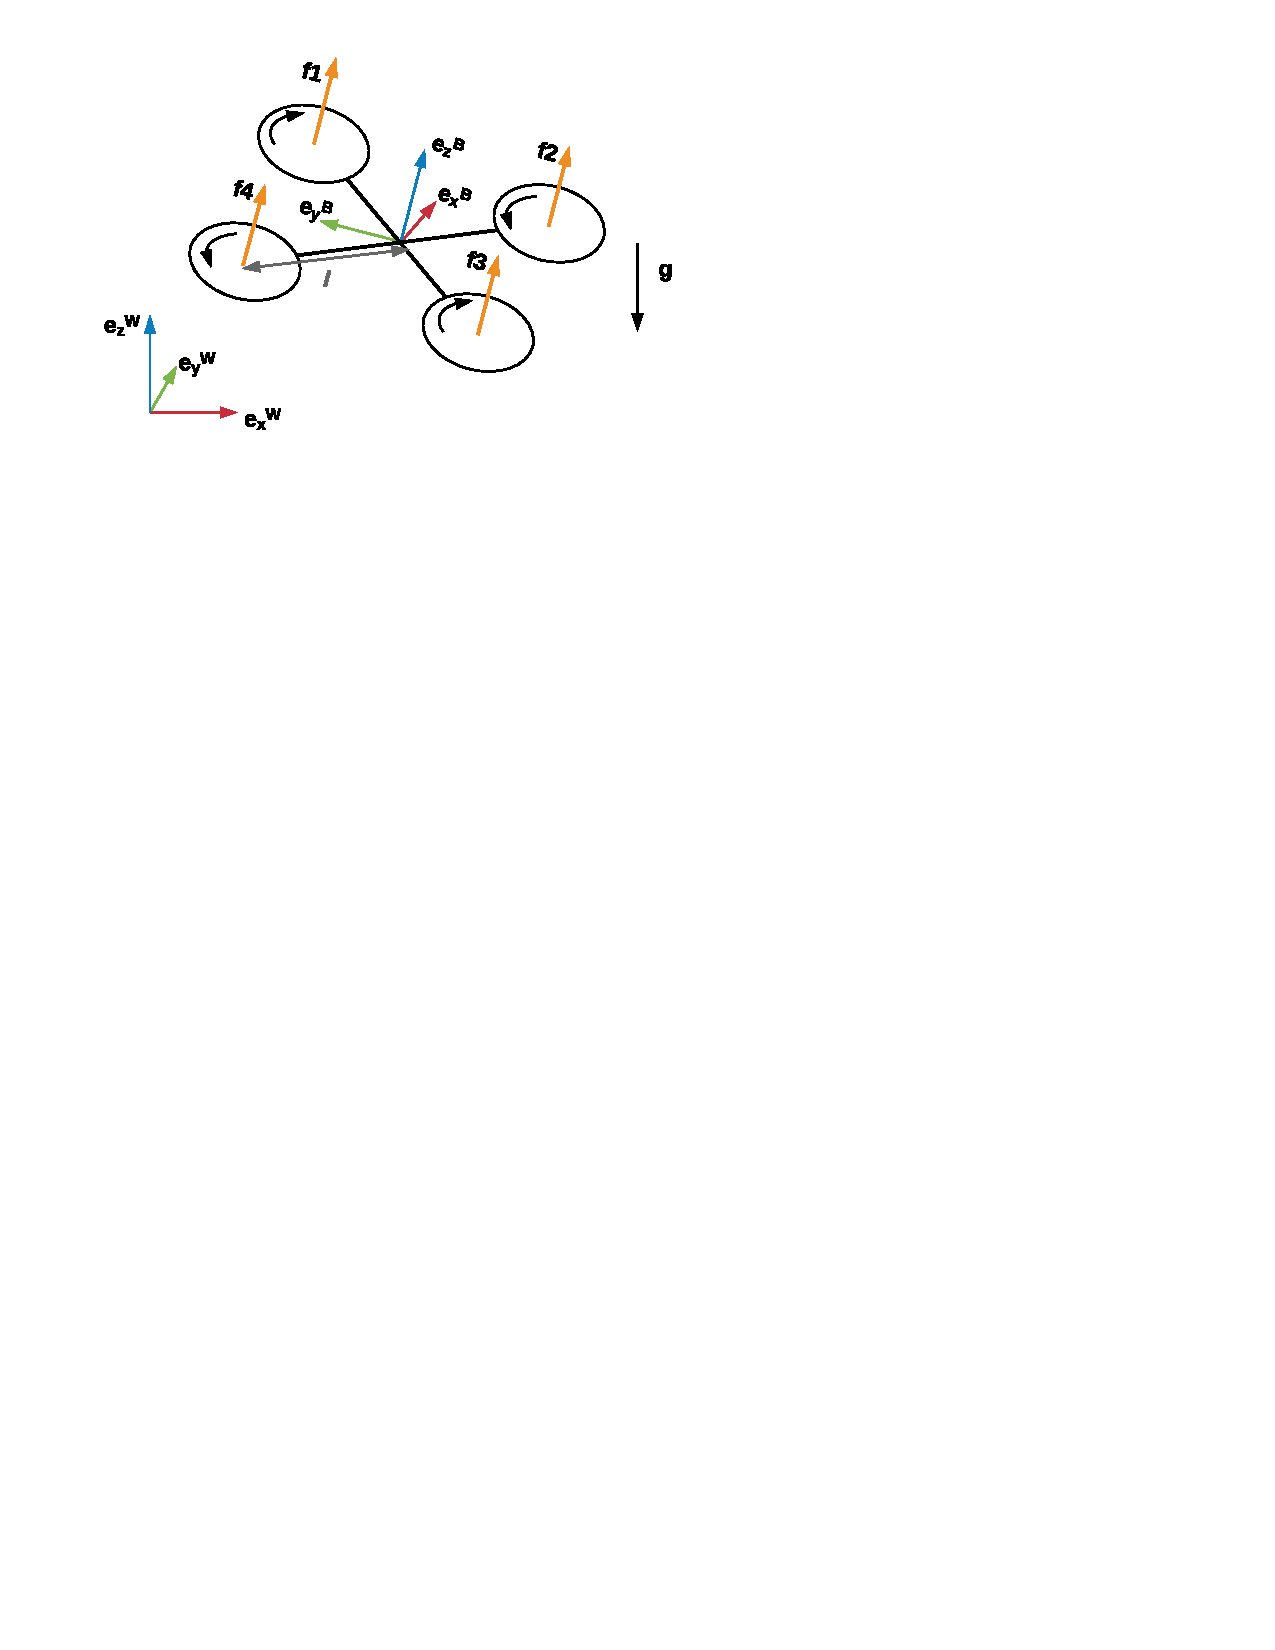
\includegraphics[width=0.7\textwidth]{img/quadrotor.pdf}
    \caption{Quadrotor with body coordinate frame and thrust forces.}
    \label{fig:bodyframe}
\end{figure}

\section{Base detection \& tracking}\label{sec:base_estimation}
In order to land on the the moving platform it is necessary to know where the base is at a specific time $t$. To do so we are using images from the camera to localize where the platform is w.r.t the quadrotor. Then, given the position of the UAV w.r.t the world frame (estimate by the module \ref{sec:state_estimation}), we can reconstruct the pose of the moving base in the global coordinate frame. \\
Now if we know how the platform should move in the world frame we can combine the noisy information from the measurements with the theoretical pose  that it should have, in order to compute a better estimation of the state of the platform.  \\
Furthermore we can predict where the platform will be in the future and use this information to plan in advance where the quadrotor must go to complete the task.\\

This module will be discussed extensively in chapter \ref{chap:base_tracking}, with explanation on all the steps we perform to have the final estimation of the base's state.

\section{State machine} \label{sec:area_exploration}
A state machine is required to differentiate the behavior of the quadrotor in the various phases of the framework. This module implements the manager that decides in which stage the UAV is, based on its pose (estimate by the module \ref{sec:state_estimation}), the position of the base (from the module \ref{sec:base_estimation}), and other inputs.\\
The main output of this module is a final desired target that the quadrotor must reach to complete the current stage and the time $T$ it should spend to arrive there.\\

This module will be discussed extensively in chapter \ref{chap:area_exploration}.


\section{Trajectory generation}
This module of the framework is taking as inputs the quadrotor state estimation (from the module \ref{sec:state_estimation}) and the final state that it has to reach (calculate by the module \ref{sec:area_exploration}) and calculate the trajectory that the UAV must track to reach the final state in $T$ seconds.\\
The trajectories are a sequence of desired positions, velocities and accelerations that the quadrotor has to reach. These desired states are given with a fixed rate to the high-controller module \ref{sec:high_control}.\\
Furthermore this module is continuously replanning the trajectories in order to compensate errors related to wrong final conditions or wrong trajectory tracking.\\  

This module will be discussed extensively in chapter \ref{chap:trajectory_generator}.

\chapter{Base Detection and Tracking}\label{chap:base_tracking}
One part of the work is focused on the estimation of the state of the moving platform. In the different phases we have to use different methods to detect and track the base:
\begin{itemize}
\item to be able to find the platform in the minimum amount of time, at the beginning, we need to inspect the area from a very high altitude. From this height we can see just a few features of the moving car and then the pose estimation are noisy. Furthermore we do not have any assumption on the initial condition of the platform, we just know the magnitude of constant forward velocity $|v_{tan}|$, so we do not know before if at a certain time $t$ the car is moving in a straight line or in a curve, we have to estimate it, and this is possible only tracking the platform for several seconds. 
\item after knowing the type of movement and a rough pose estimation of the moving car, we can use these information to improve our state estimation: getting close to the platform without loosing the tracking, starting a more precise measure (base on tag detection), and filtering the measurements with a theoretical model of the movement.
\end{itemize}

\section{From high altitude}
To find the car we assume that the platform is the only white square moving on the arena.
Base on this assumption, we analyze the images from the down looking camera to find a moving white square and calculate its optical flow to predict its future position.
We perform the following passages:
\begin{itemize}
\item threshold the image in order to find the white features.
\item find all the close shapes in the image.
\item select only the shapes with
\begin{itemize}
\item 4 edges
\item convex contour
\item angles between edges close to $\frac{\pi}{2}$
\end{itemize}
\end{itemize}
At this point we have the position of the four corners of all the squares in the image.\\
Now we try to calculate the optical flow of these points through the sequence of images and we track only the points that are moving with a velocity comparable to the one known $v_{tan}$.\\
To perform the optical flow we use the Lucas-Kanade method. %TODO citazione
It assumes that the displacement of the image contents between two nearby frames is small and approximately constant within a neighborhood of the point p under consideration. Thus the optical flow equation can be assumed to hold for all pixels within a window centered at $p$. Namely, the local image flow vector $(V_{x},V_{y})$ must satisfy:

\begin{align}
\begin{split}
I_{x}(q_{1})V_{x}+I_{y}(q_{1})V_{y}=-I_{t}(q_{1})  \\
I_{x}(q_{2})V_{x}+I_{y}(q_{2})V_{y}=-I_{t}(q_{2})  \\
\vdots \\
I_{x}(q_{n})V_{x}+I_{y}(q_{n})V_{y}=-I_{t}(q_{n}) 
\end{split}
\end{align}

Where $q_{1},q_{2},\dots ,q_{n}$ are the pixels inside the window, and $I_{x}(q_{i}),I_{y}(q_{i}),I_{t}(q_{i})$ are the partial derivatives of the image $I$ I with respect to position x, y and time t, evaluated at the point $q_{i}$ and at the current time.\\
These equations can be written in matrix form $Av=b$, where
\begin{align}
A={\begin{bmatrix}I_{x}(q_{1})&I_{y}(q_{1})\\[10pt]I_{x}(q_{2})&I_{y}(q_{2})\\[10pt]\vdots &\vdots \\[10pt]I_{x}(q_{n})&I_{y}(q_{n})\end{bmatrix}},\quad \quad v={\begin{bmatrix}V_{x}\\[10pt]V_{y}\end{bmatrix}},\quad {\mbox{and}}\quad b={\begin{bmatrix}-I_{t}(q_{1})\\[10pt]-I_{t}(q_{2})\\[10pt]\vdots \\[10pt]-I_{t}(q_{n})\end{bmatrix}}
\end{align}

This system has more equations than unknowns and thus it is usually over-determined. The Lucas-Kanade method obtains a compromise solution by the least squares principle. Namely, it solves the $2\times2$ system:
\begin{align}
\begin{split}
A^{T}Av=A^{T}b\\
{\mathrm  {v}}=(A^{T}A)^{{-1}}A^{T}b
\end{split}
\end{align}
\begin{align}
{\begin{bmatrix}V_{x}\\[10pt]V_{y}\end{bmatrix}}={\begin{bmatrix}\sum _{i}I_{x}(q_{i})^{2}&\sum _{i}I_{x}(q_{i})I_{y}(q_{i})\\[10pt]\sum _{i}I_{y}(q_{i})I_{x}(q_{i})&\sum _{i}I_{y}(q_{i})^{2}\end{bmatrix}}^{{-1}}{\begin{bmatrix}-\sum _{i}I_{x}(q_{i})I_{t}(q_{i})\\[10pt]-\sum _{i}I_{y}(q_{i})I_{t}(q_{i})\end{bmatrix}}
\end{align}
With this method we can track the interesting points from frame to frame, calculate direction and velocity of the car and so predict where it will be after a time $t$.\\
\begin{figure}[!htbp]
  \centering
  {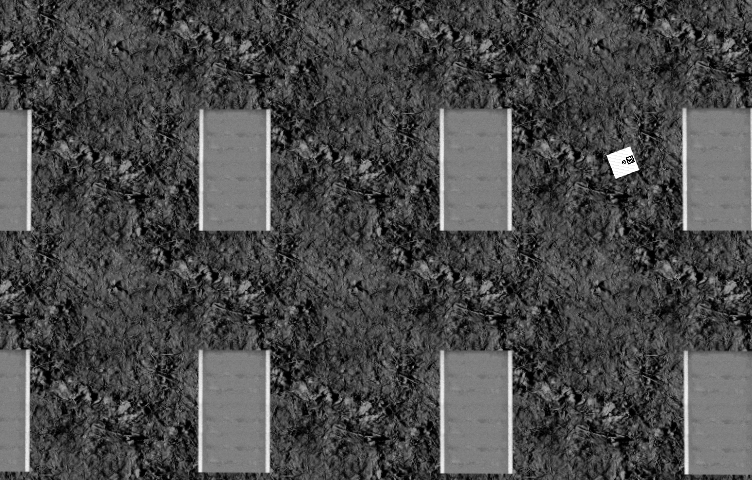
\includegraphics[width=0.45\textwidth]{img/18730previousImage.png}\label{fig:original}}
  \hfill
  {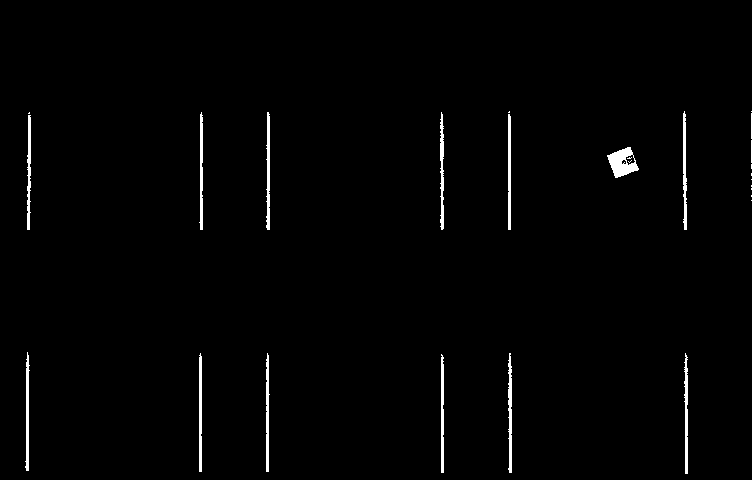
\includegraphics[width=0.45\textwidth]{img/18730_thresholded.png}\label{fig:threshold}}
  \vspace{1cm}
  
  {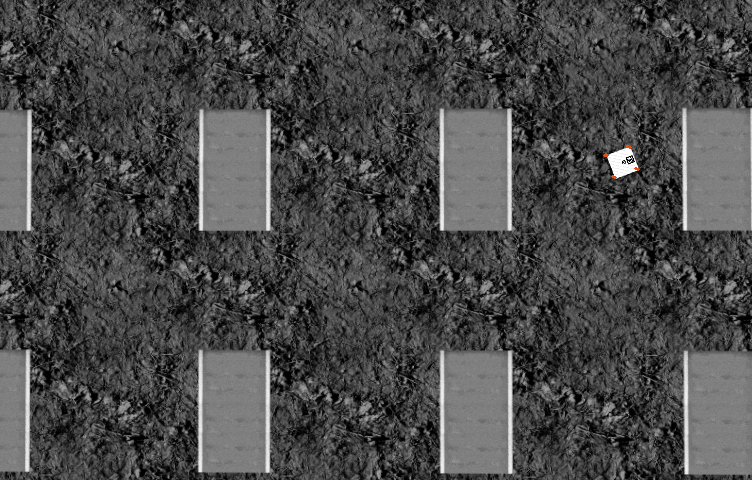
\includegraphics[width=0.45\textwidth]{img/18741_optical_flow.png}\label{fig:optical1}}
  \hfill
  {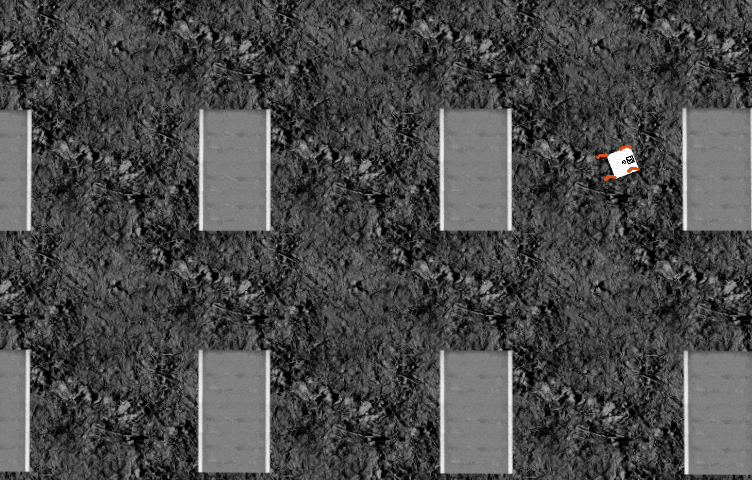
\includegraphics[width=0.45\textwidth]{img/18758_optical_flow.png}\label{fig:optical2}}
  \vspace{1cm}
  
  {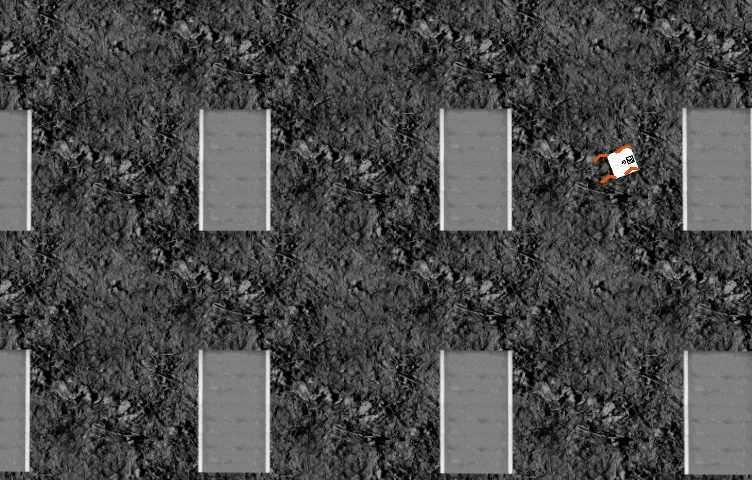
\includegraphics[width=0.45\textwidth]{img/18777_optical_flow.png}\label{fig:optical3}}
  \hfill
  {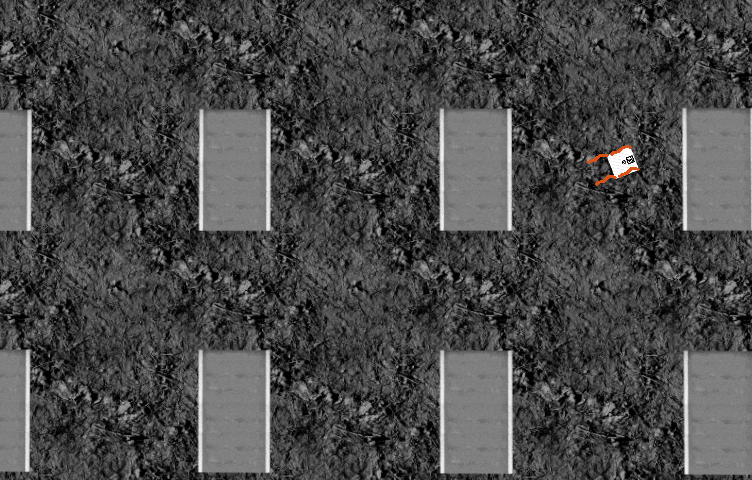
\includegraphics[width=0.45\textwidth]{img/18800_optical_flow.png}\label{fig:optical4}}
   
  \vspace{1cm}
  {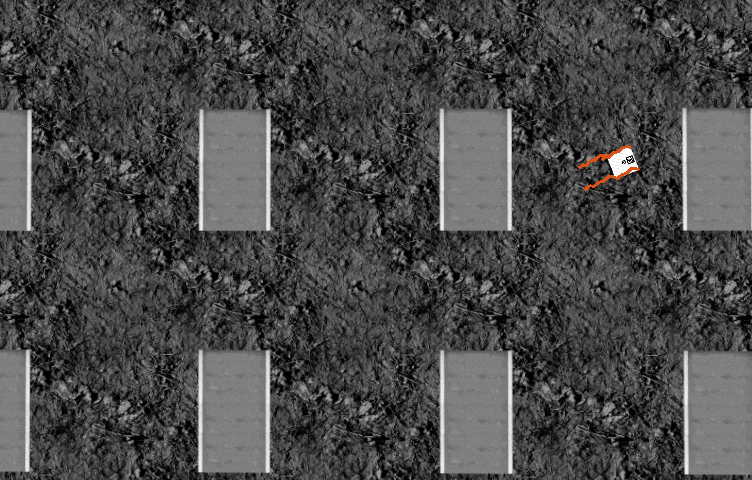
\includegraphics[width=0.45\textwidth]{img/18856_optical_flow.png}\label{fig:optical5}}
  \hfill
  {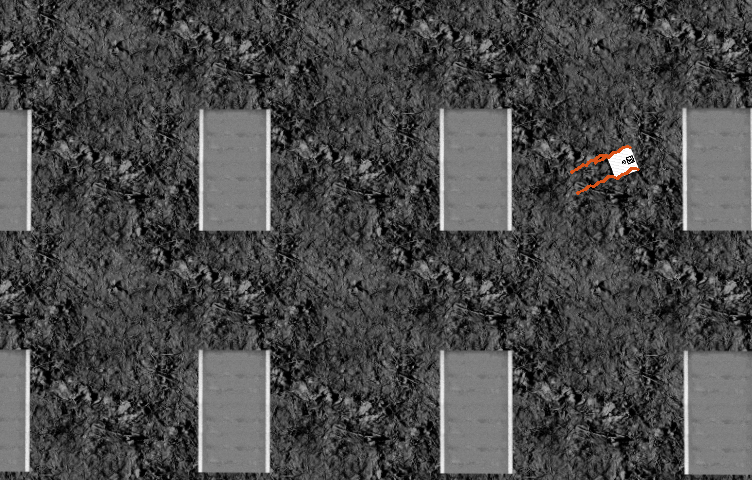
\includegraphics[width=0.45\textwidth]{img/18881_optical_flow.png}\label{fig:optical6}}
 
  \caption{A sequence of images where the moving car is detected and tracked. First image is the original image. Then the one after thresholding. Then all the subsequent images where the corners of the platform are tracked.}
  \label{fig:optical_folw_sequence}
\end{figure} 

\subsubsection{From images to real world}
After tracking the platform in the images, we have to find its position in the 3D real world. This position is calculate using the pinhole model of the camera: %TODO citazione
\begin{align}
wm = A [R|t]M
 \label{eq:pinholemodel}
\end{align}
In expanded form:
\begin{align}
{w\begin{bmatrix}
u \\[10pt]
v  \\[10pt]
1
\end{bmatrix}}=
{\begin{bmatrix}\
f_x & 0 & c_x \\[10pt]
0 & f_y &c_y \\[10pt]
0 & 0 & 1
\end{bmatrix}}
{\begin{bmatrix}\
r_{11} & r_{12} & r_{13} & t_{x} \\[10pt]
r_{21} & r_{22} & r_{23} & t_{y} \\[10pt]
r_{31} & r_{32} & r_{33} & t_{z}
\end{bmatrix}}
{\begin{bmatrix}
X \\[10pt]
Y \\[10pt]
Z \\[10pt]
1
\end{bmatrix}}
\end{align}
Where:
\begin{itemize}
 \item $m$ homogeneous coordinate of the projection point in pixel.
  \item $M$ homogeneous coordinate of a 3D point in the world coordinate frame.
 \item $A$ is the camera matrix or the matrix of intrinsic parameters. It is Composed by $f_x,f_y$ the focal lengths and $c_x,c_y$ the principal point.
 \item $[R|t]$ is the joint rotation-translation matrix or matrix of extrinsic parameters. It express the camera motion around the static scene. This matrix denote the coordinate system transformations from 3D world coordinates to 3D camera coordinates. The position $C$ of the camera expressed in world coordinates is $C=-R^{{-1}}t=-R^{T}t$.
\end{itemize}

We can calculate the depth of the platform using the known dimension of the base: given the length $l_w$ of the square in the real world and the average dimension of the edges in the image $l_i$, we can calculate the depth with respect to the camera frame 
\begin{align}
z = \frac{l_w f}{l_i}
\end{align}
To calculate the dimension $l_i$ we need at least 3 corner of the base and we calculate all the pairwise distances between the corners \ref{fig:platform_profile}:
\begin{itemize}
\item if we have 4 corners there are 6 different distances: 4 of which equal to $l_i$ and 2 $\sqrt{2}l_i$
\item if we have 3 corners there are 3 different distances: 2 of which equal to $l_i$ and 1 $\sqrt{2}l_i$
\end{itemize}
This approximation is not really precise when we see the platform with a camera not perpendicular to the base, but we need just a rough approximation of the height in this first phase.
\begin{figure}[!htbp]
  \centering
  {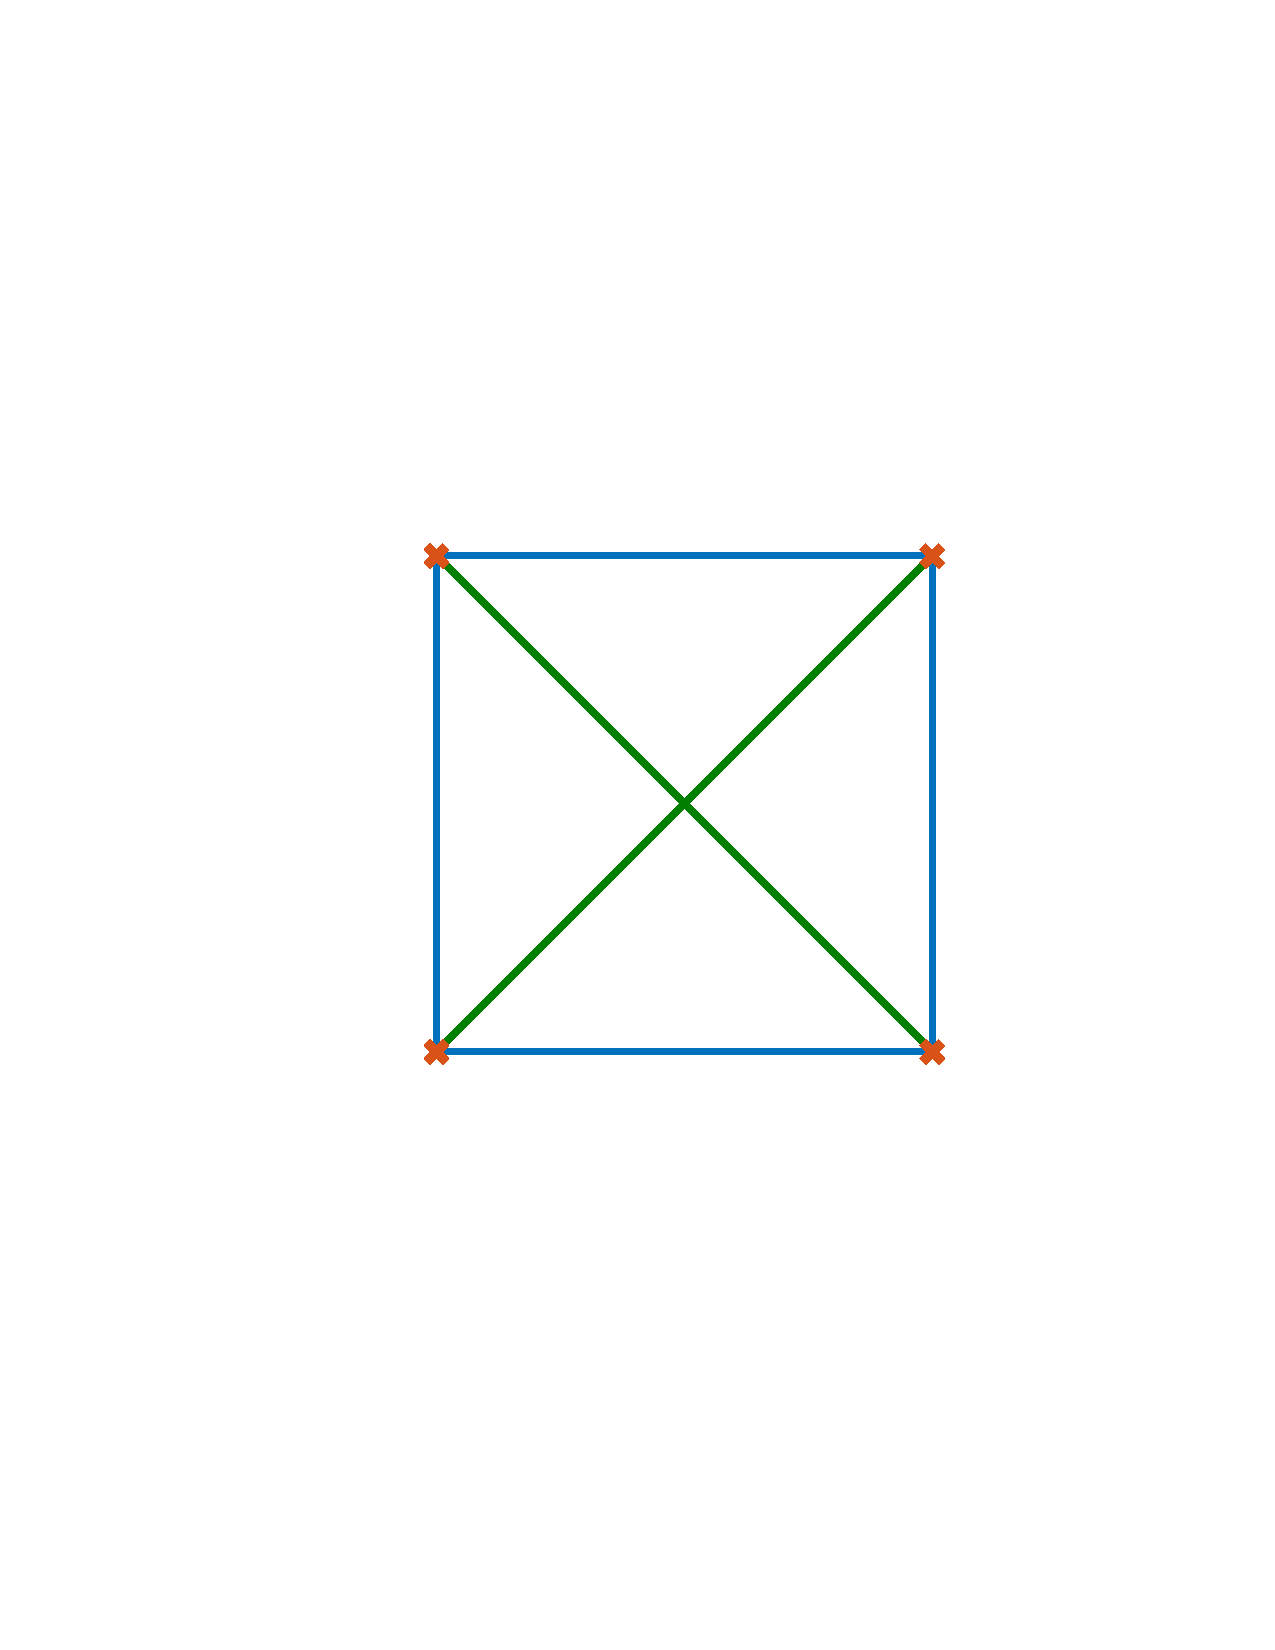
\includegraphics[width=0.3\textwidth]{img/platform_4_edges.pdf}\label{fig:4_corners}}
  \hspace{5em}
  {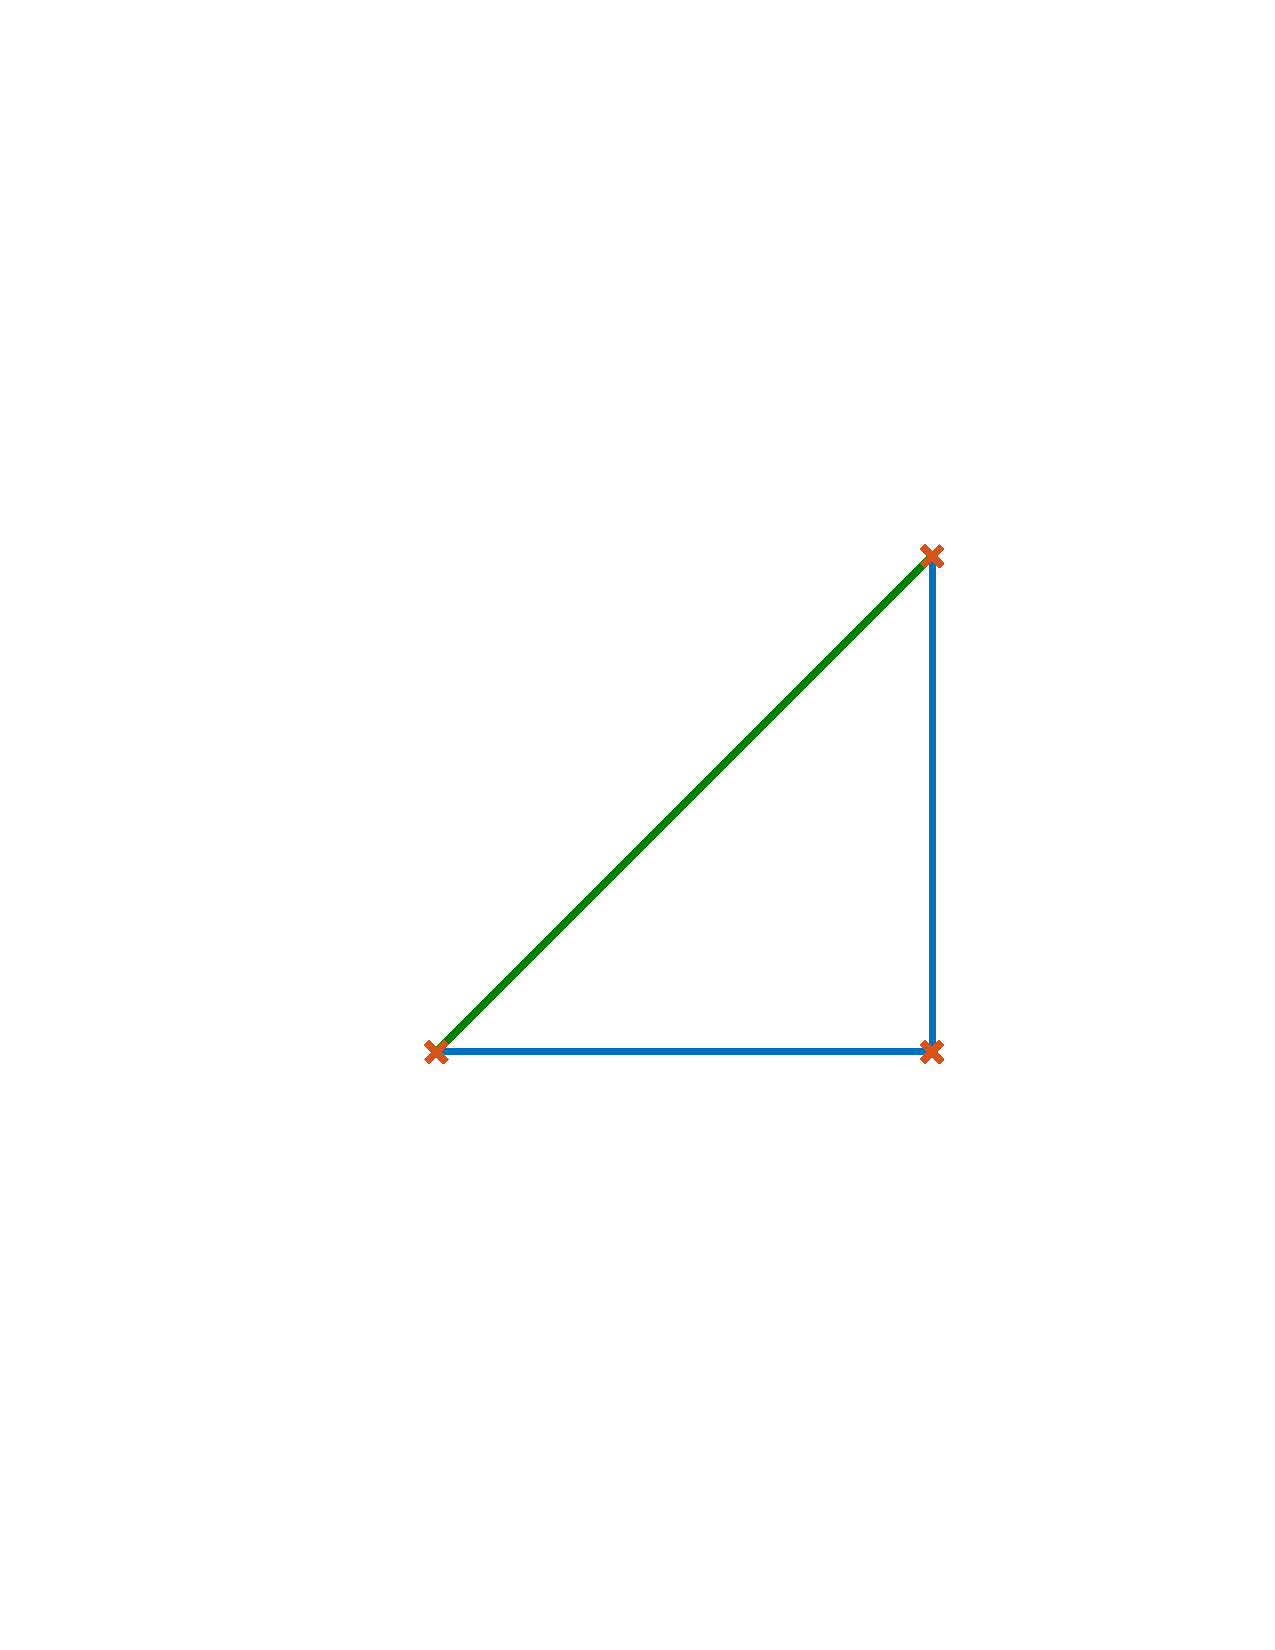
\includegraphics[width=0.3\textwidth]{img/platform_3_edges.pdf}\label{fig:3_corners}}
  \caption{Model of the square platform detected on the image. Red crosses corner detected. Blue lines edges with length $l_i$. Green lines edges with length $\sqrt{2}l_i$ }
  \label{fig:platform_profile}
\end{figure} 

If this depth $z!=0$ we can  solve the system of equation \ref{eq:pinholemodel} finding an unique solution using the following equivalent equations:
\begin{align}
\begin{split}
x &= z\frac{u-c_x}{f_x}\\[10pt]
y &= z\frac{u-c_y}{f_y}\\[10pt]
{\begin{bmatrix}
x \\[10pt]
y \\[10pt]
z
\end{bmatrix}} &= 
R {\begin{bmatrix}
X \\[10pt]
Y \\[10pt]
Z
\end{bmatrix}} + t
\end{split}
\end{align}

A better method to find the position of the platform, without the approximation of the depth $z$ is to resolve a Perspective-n-Point problem %TODO cite
that estimates the pose of a camera given a set of n 3D points in the world and their corresponding 2D projections in the image. The only issue is that to solve this problem without ambiguity the minimum number of points is 4, and sometimes we can track only 3 corners of the base, but when all the 4 points are available we solve the correspondent PnP problem to find a better estimation of the base position.\\

With this method every time we detect the car we can estimate its position and velocity vector in world coordinate frame, so  we can predict where the platform will be in $t$ seconds and where the quadrotor should go to following the base.\\

\section{From low altitude}

\subsection{Extended Kalman Filter}
An Extended Kalman Filter is design in order to have the most reliable value of the state of the platform.

Kalman filtering is an algorithm that uses a series of noisy measurements observed over time and produces estimates of unknown variables that tend to be more precise than those based on a single measurement alone, by using Bayesian inference and estimating a joint probability distribution over the variables for each time frame.\\
The algorithm works in a two-step process:
\begin{itemize}
\item In the prediction step, the Kalman filter produces estimates of the current state variables, along with their uncertainties, based on a model of the system:
\begin{equation}
\boldsymbol{x}_k = f(\boldsymbol{x}_{k-1},\boldsymbol{u}_k) + \boldsymbol{w}_k
\end{equation}
\item Once the outcome of the next measurement is observed:
\begin{equation}
\boldsymbol{z}_k = h(\boldsymbol{x}_{k}) + \boldsymbol{v}_k
\end{equation}
these estimates are updated using a weighted average, with more weight being given to estimates with higher certainty.
\end{itemize}
In the extended Kalman filter, the state transition and observation models don't need to be linear functions of the state but may instead be differentiable functions.\\
($\boldsymbol{w}_k$ and $\boldsymbol{v}_k$ are the process and observation noises which are both assumed to be zero mean multivariate Gaussian noises with covariance $\boldsymbol{Q}_k$ and $\boldsymbol{R}_k$ respectively. $\boldsymbol{u}_k$ is the control vector).

  The algorithm is recursive. It can run in real time, using only the present input measurements and the previously calculated state and its uncertainty matrix; no additional past information is required.\\
The Kalman filter does not require any assumption that the errors are Gaussian. However, the filter yields the exact conditional probability estimate in the special case that all errors are Gaussian-distributed.\\
Initialization
\begin{align}
\begin{split}
\boldsymbol{x}_{0|0} = x_0\\
\boldsymbol{P}_{0|0} = P_0
\end{split}
\end{align}
In this case the prediction equations are continuous in time, so for the prediction step of the EKF we have to solve:
\begin{align}
\begin{split}
\boldsymbol{\dot{\hat{x}}}(t) &= f(\boldsymbol{\hat{x}}(t),\boldsymbol{u}(t)) \\
\boldsymbol{\dot{P}}(t) &= \boldsymbol{F}(t) \boldsymbol{P}(t) + \boldsymbol{P}(t)\boldsymbol{F}(t)^{\top } + \boldsymbol{Q}(t)
\end{split}
\end{align}
for $t \in (t_{k-1}, t_k)$ where %TODO
\begin{align}
\begin{split}
\boldsymbol{\hat{x}}(t_{k-1}) &= \hat{x}_{k-1|k-1} \\
\boldsymbol{P}(t_{k-1}) &= P_{k-1|k-1}
\\
{\boldsymbol{F}}(t)&=\left.{\frac  {\partial f}{\partial {\boldsymbol{x}}}}\right\vert _{{{\hat  {{\boldsymbol{x}}}}(t),{\boldsymbol{u}}(t)}}  \\
\boldsymbol{\hat{x}}_{k|k-1} &= \boldsymbol{\hat{x}}(t_{k}) \\
\boldsymbol{P}_{k|k-1} &= \boldsymbol{P}(t_{k})
\end{split}
\end{align}
In order to save some computation we can discretize the dynamicin order to have shorter computation during the prediction step of the EKF:
\begin{align}
\begin{split}
\boldsymbol{\hat{x}}_{k|k-1} &= f(\boldsymbol{\hat{x}}_{k-1|k-1},\boldsymbol{u}_k) \\
\boldsymbol{P}_{k|k-1} &= \boldsymbol{F}_{k-1} \boldsymbol{P}_{k-1|k-1}\boldsymbol{F}_{k-1}^{\top } + \boldsymbol{Q}_{k}
\end{split}
\end{align}
where the state transition matrix is defined to be the following Jacobians:
\begin{align}
\begin{split}
\boldsymbol{F}_{k-1}&= \left.{\frac{\partial f}{\partial {\boldsymbol{x}}}} \right \vert_{\hat{\boldsymbol{x}}_{k-1|k-1},\boldsymbol{u}_{k}} 
\end{split}
\end{align}
While the update equations are discrete in time and they yield to the following update step: 
\begin{align}
\begin{split}
\boldsymbol{K}_{k} &= \boldsymbol{P}_{k|k-1} \boldsymbol{H}_{k}^{\top }(\boldsymbol{H}_{k} \boldsymbol{P}_{k|k-1} \boldsymbol{H}_{k}^{\top }+ \boldsymbol{R}_{k})^{-1}
\\
\hat{\boldsymbol{x}}_{k|k} &= \hat{\boldsymbol{x}}_{k|k-1} + \boldsymbol{K}_{k} (\boldsymbol{z}_{k}-h(\hat{\boldsymbol{x}}_{k|k-1}))
\\
\boldsymbol{P}_{k|k} &=(\boldsymbol{I}-\boldsymbol{K}_{k}\boldsymbol{H}_{k})\boldsymbol{P}_{k|k-1}
\end{split}
\end{align}
where the observation matrix is defined to be the following Jacobian:

\begin{align}
\begin{split}
\boldsymbol{H}_{k} = \left.{\frac{\partial h}{\partial {\boldsymbol{x}}}} \right \vert_{\hat{\boldsymbol{x}}_{k|k-1}}
\end{split}
\end{align}

\subsubsection{Prediction update: non-holonomic model}
The platform is considered as a car and simulated with a non-holonomic model. 
In this model the state is defined as $\boldsymbol{x} = (x, y, z,\theta , v, \phi)$:
It corresponds to the 3 position in a space $(x,y,z)$ and the yaw angle of the platform $(\theta)$ w.r.t. the world frame, the forward velocity ($v$) and the angle of the front wheels ($\phi$). The system depends on a parameter $L$ that corresponds to the distance between the front and the back wheels.\\
In this model the control input are the change in velocity $v$ and in the angle of curvature $\phi$. \\
The equation of motion in continuous time are:
\begin{align}
\boldsymbol{\dot{x}} = f(\boldsymbol{x},\boldsymbol{u}) \nonumber
\end{align}
\begin{align}
\begin{split}
\dot{x} &= v cos(\theta) \\
\dot{y} &= v sin(\theta) \\
\dot{z} &= 0 \\
\dot{\theta} &= \frac{v}{L}tan(\phi)\\
\dot{v} &= u_1 \\
\dot{\phi} &= u_2 
\end{split}
\end{align}
It is possible to discretize these dynamics in $t \in (t_{k-1}, t_k)$ with a first order finite difference:
\begin{align}
\boldsymbol{\dot{x}} \approx \frac{\boldsymbol{x}_k - \boldsymbol{x}_{k-1} }{dt} \approx f(\boldsymbol{x}_{k-1},\boldsymbol{u}_k) \nonumber
\end{align}
with $\boldsymbol{x}_k = \boldsymbol{x}(t_k)$, $\boldsymbol{x}_{k-1} = \boldsymbol{x}(t_{k-1})$, $dt = t_k - t_{k-1}$
\begin{align}
\begin{split}
x_k &= x_{k-1} + dt \big(v_{k-1} cos(\theta_{k-1})\big) \\
y_k &= y_{k-1} + dt \big(v_{k-1} sin(\theta_{k-1})\big) \\
z_k &= z_{k-1} \\
\theta_k &= \theta_{k-1} + dt\Big(\frac{v_{k-1}}{L}tan(\phi_{k-1}) \Big)\\
v_{k} &= v_{k-1} + dt \big(u_{1k}\big) \\
\phi_k &= \phi_{k-1} + dt \big(u_{2k}\big) 
\end{split}
\end{align}
In order to solve the former system, we have anyway to find a numerical solution. For this purpose we use a    
RUNGE-KUTTA scheme %TODO
\begin{figure}[!ht]
    \centering
    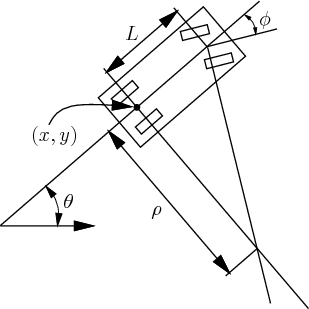
\includegraphics[width=0.5\textwidth]{img/non_holonomic_model.png}
    \caption{Non-holonomic model}
    \label{fig:nonholonomicmodel}
\end{figure}
\paragraph{Straight and circular path}
For now we assume the input $u_1$ and $u_2$  are equal to zero, so the platform can be static ($v_f(0) = 0$) can move in a straight line ($v_f(0) \neq 0$ and $\phi(0) = 0$) or in a circle ($v_f(0) \neq 0$ and $\phi(0) \neq 0$)


\subsection{Measurement update}
\subsubsection{Tag Detector}

\paragraph{April Tag vs Ar Sys}
precision comparison vs frequency
nodlet
\subsubsection{Cross Detector}
pnp problem
\subsubsection{Covariance Estimation}



\section{Results}
\begin{figure}[!ht]
    \centering
    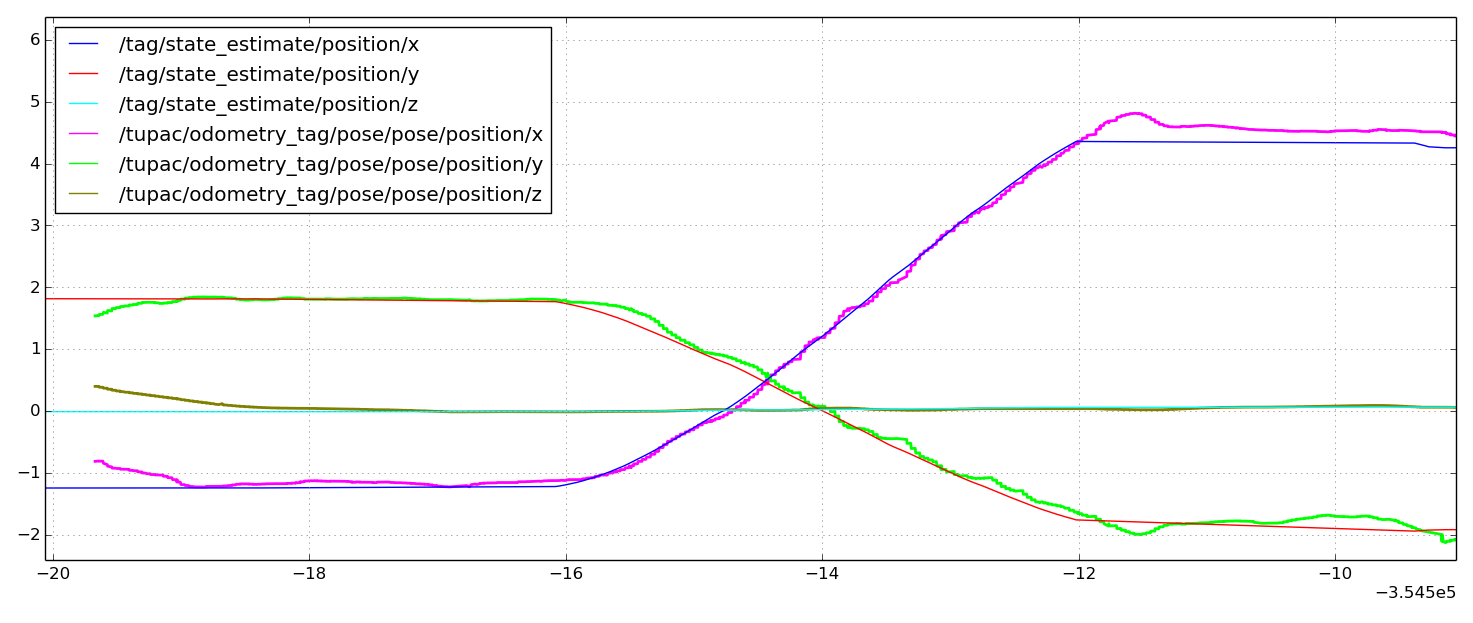
\includegraphics[width=0.97\textwidth]{img/position_real_world_fast.png}
    \caption{EKF 1}
    \label{fig:ekf_position_fast}
\end{figure}
\begin{figure}[!ht]
    \centering
    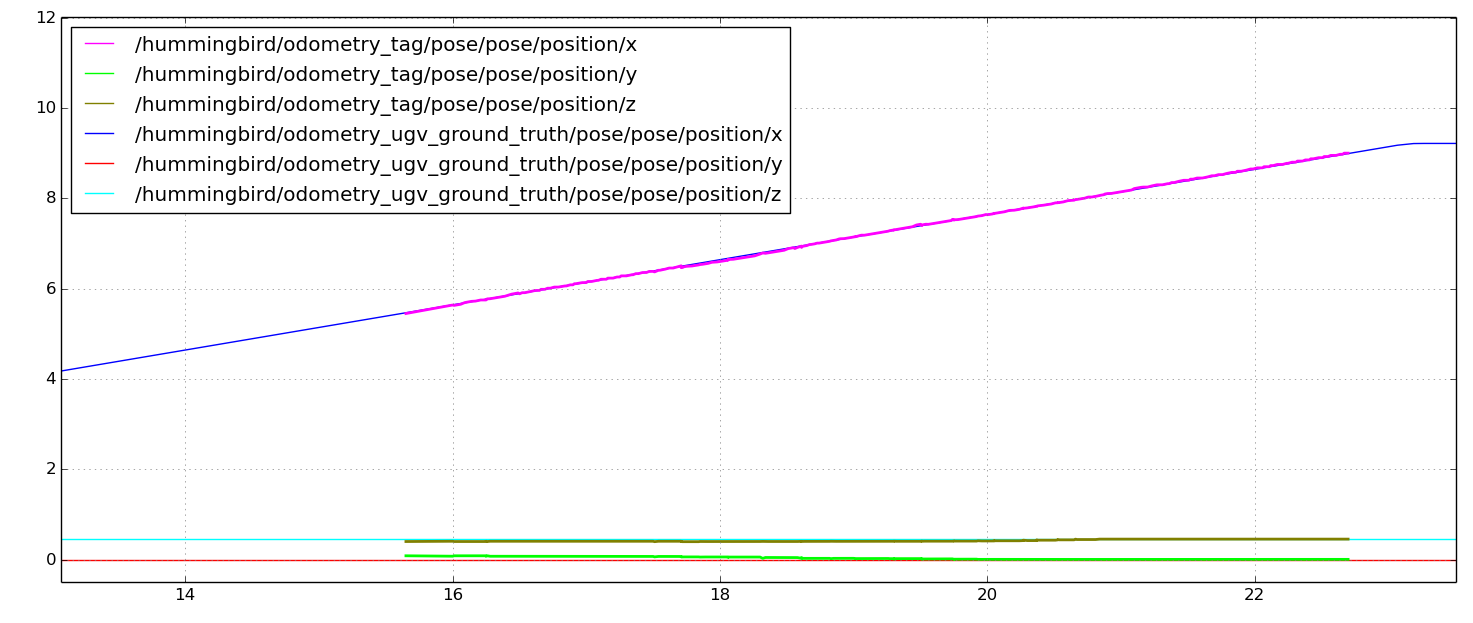
\includegraphics[width=0.97\textwidth]{img/position_simulation_hot_init.png}
    \caption{EKF 2}
    \label{fig:ekf_position_hot_init}
\end{figure}

\chapter{Area exploration}\label{chap:area_exploration}
different time exploration
imu to switch off
time following

\section{State machine}


\begin{figure}[!ht]
    \centering
    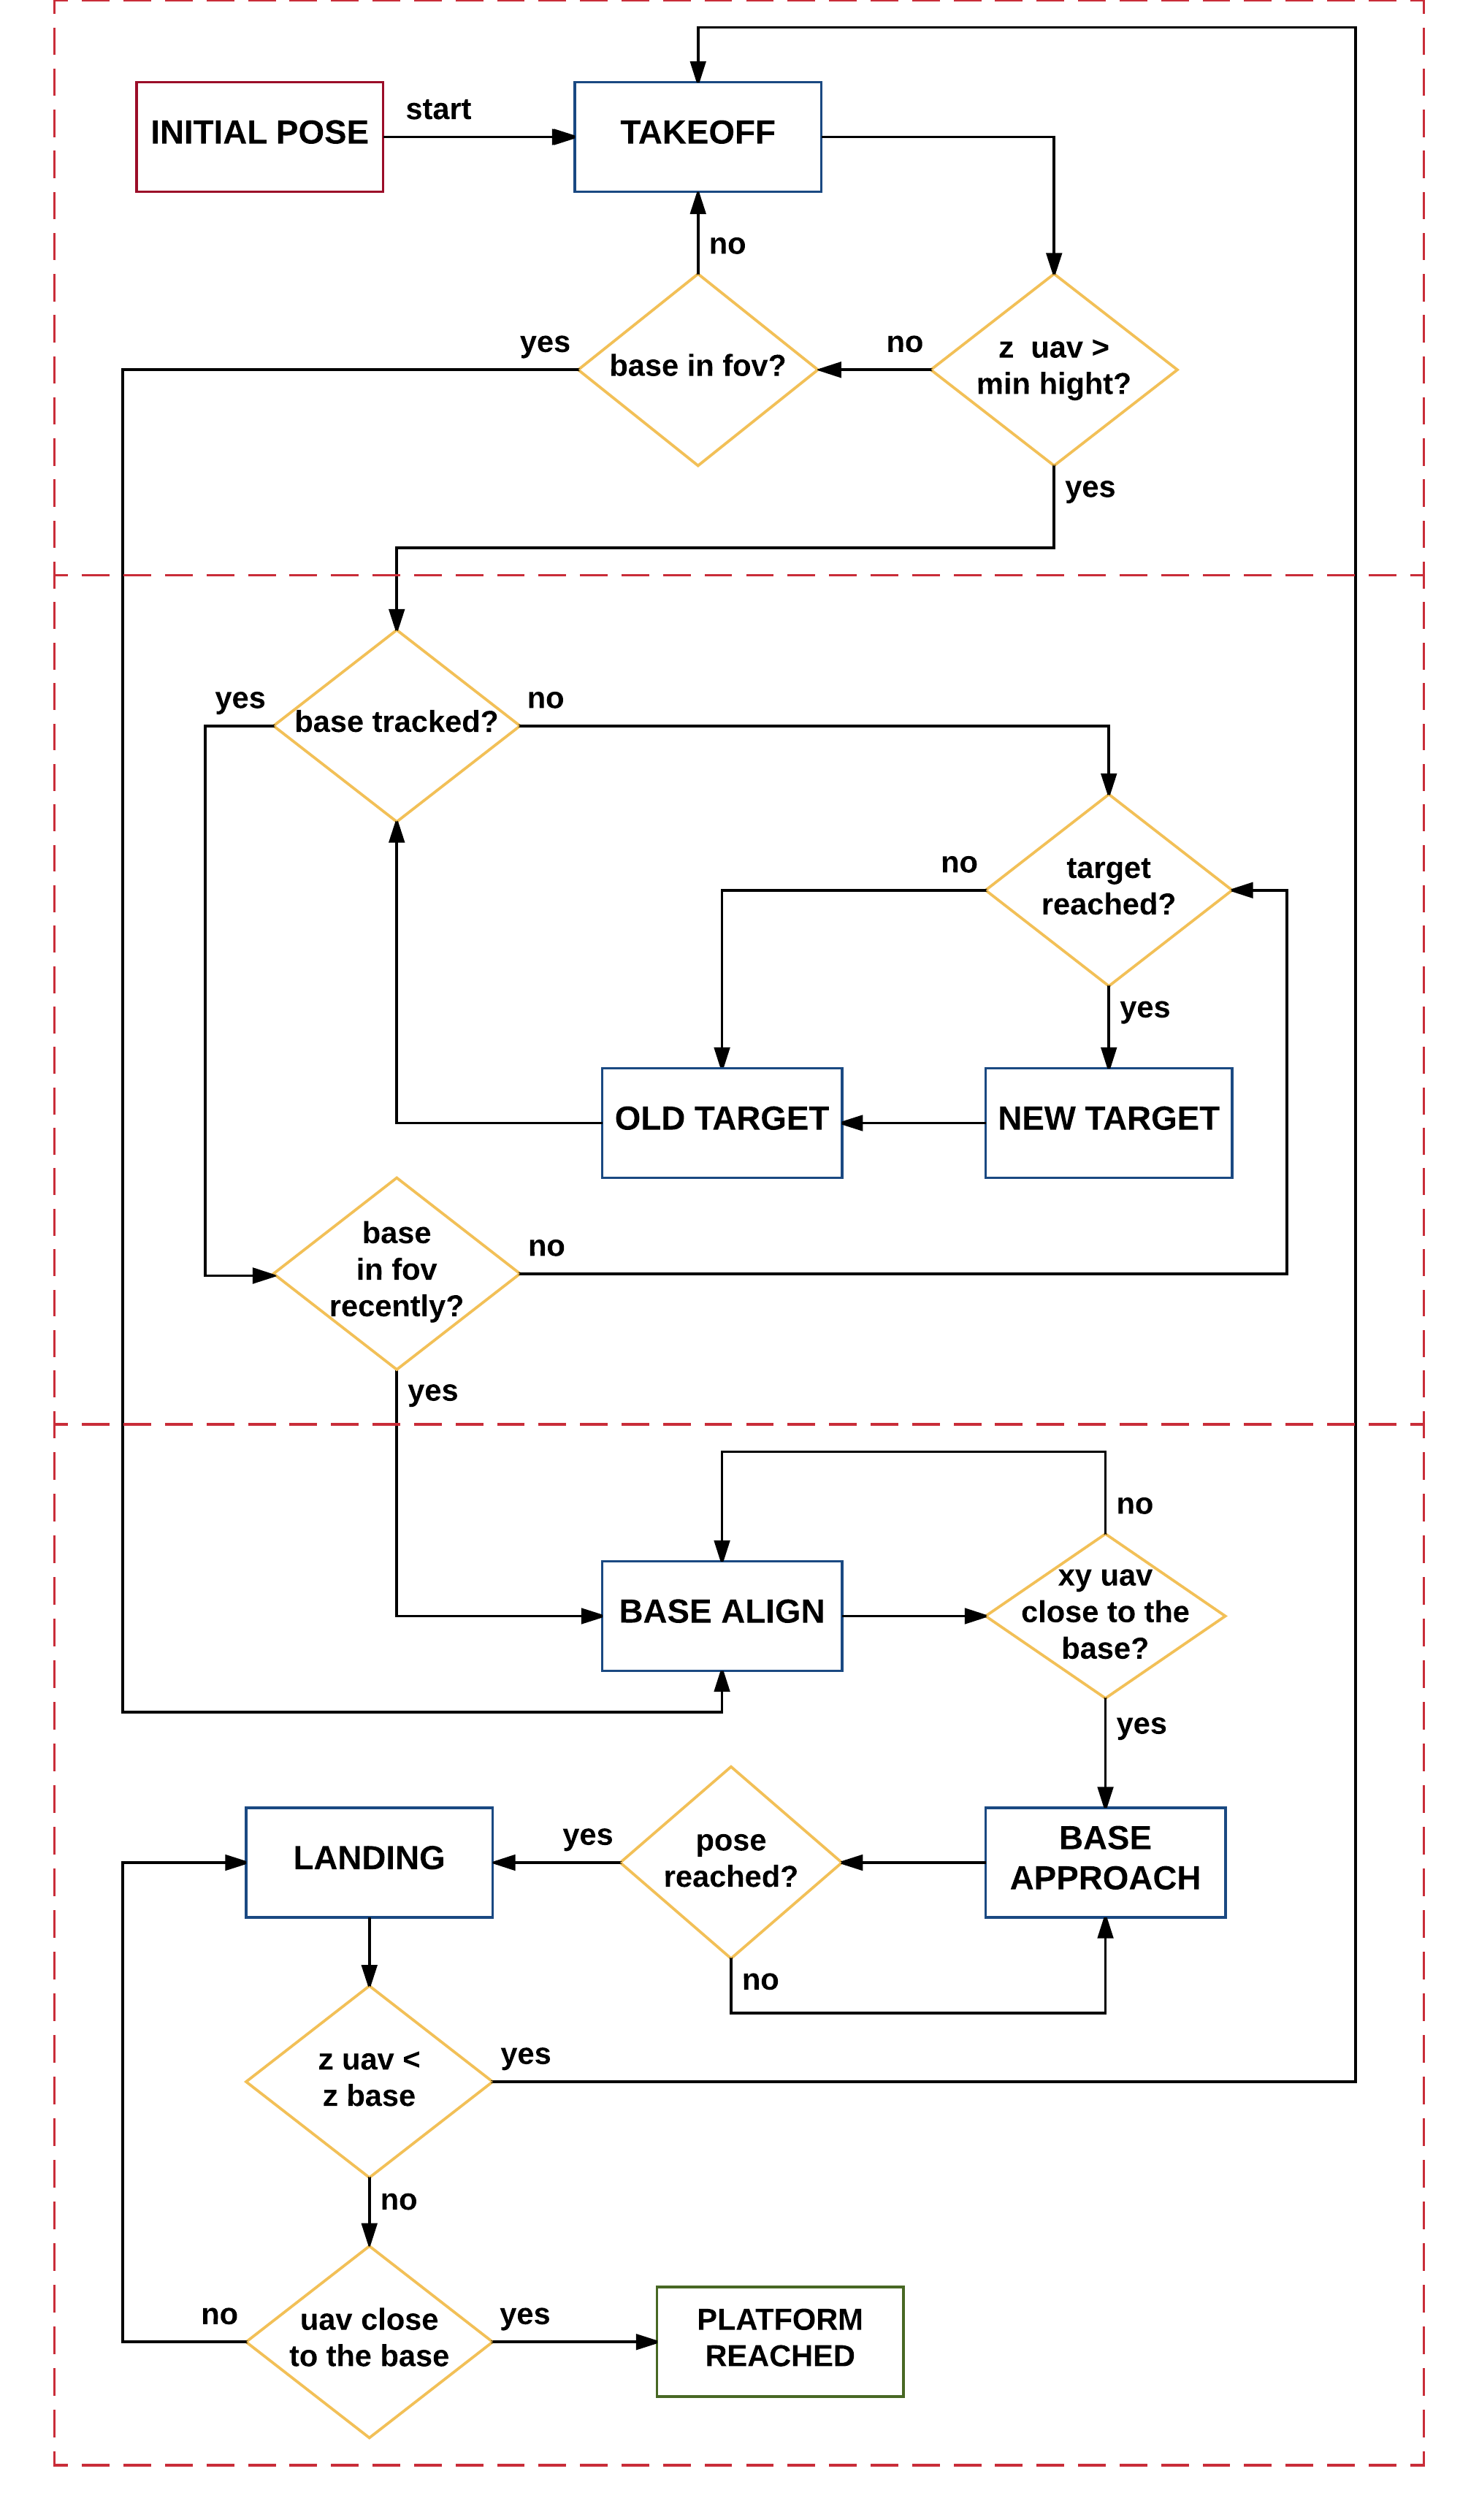
\includegraphics[width=0.97\textwidth]{img/area_exploration_state_machine.png}
    \caption{Area Exploration}
    \label{fig:area_exploration_state_machine}
\end{figure}

\subsection{Phases}
\subsubsection{First phase - Searching for the base}
In this phase the quadrotor starts from a given position and has to find the moving car.
Given the rectangle in which the platform can move the UAV follows a list of way-points in order to span the whole area at high altitude. In this way the downward camera can collect information from a large section of the space and the searching of the base is faster.\\
To find the platform we have the following assumptions:
\begin{itemize}
\item the platform is the only white square moving on the arena
\item in a small period of time the movement of the platform is approximable with a linear motion  
\end{itemize}

Base on these assumptions, we analyze the images from the down looking camera to find a moving white square and calculate its optical flow to predict its future position.
We perform the following passages:
\begin{itemize}
\item threshold the image in order to find the white features
\item find the edges with the canny edge algorithm
\item find the connected edges that define contours of shapes
\item select only the shapes with 4 edges
\item check if the edges have the same length 
\item check if the angle between edges is $\frac{\pi}{2}$
\end{itemize}
At this point we have the position of the squares in the image.\\
Now we try to calculate the optical flow of these points through the sequence of images and we track only the points that are moving with a velocity comparable to the one known. We can calculate the direction of the platform and then predict where it will be after a time $t$.
 

\subsubsection{Second phase - Approaching the base}

\subsubsection{Second phase - Following the base}

\subsubsection{Second phase - Landing on the base}

\chapter{Trajectory Generator}\label{chap:trajectory_generator}
This section describes the module that computes the trajectory the vehicle has to execute to accompish the task of landing on a moving platform.\\

A trajectory is a sequence of desired states that leads the UAV from an initial condition at $t = t_0 $ to the desired final condition reached at $t = T$. In particular, a desired state at a certain time $t_i$ is defined as:
 \begin{itemize}
\item $[p_{x,t_i,des},p_{y,t_i,des},p_{z,t_i,des}]$: desired 3D position;
\item $[v_{x,t_i,des},v_{y,t_i,des},v_{z,t_i,des}]$: desired linear velocity;
\item $[a_{x,t_i,des},a_{y,t_i,des},a_{z,t_i,des}]$: desired linear acceleration;
\item $[\psi_{t_i,des}]$: desired yaw.
\end{itemize}
The fact that the desired state of the quadrotor is completely defined by these quantities is because the quadrotor dynamics are differentially flat \cite{van1997real}: the states and the inputs can be written as algebraic functions of four flat outputs and their derivatives: $[x,y,z,\psi]$.\\

The initial desired state, for $t_i = t_0$, is given by the state estimation of the quad, while the final condition for $t_i = T$ are given from the state machine module. \\

The final conditions can be of different types, and the calculation of the possible trajectories depends on them:
\begin{itemize}
\item During the first two stages of the state machine, the final state is simply a pose in the world frame with zero velocity and acceleration. This module computes some trajectories from the initial state to this final states with different total times $T_i$ and it is choosing the one that is minimizing a specific cost function. We will see in the following sections, the different cost functions that can be chosen.\\ 
The times $T_i$ depend on the distance between initial and final position, and the average velocity that the quad should have during the flight.
\item During the third stage, the final state is a pose in the world frame with a velocity equal to the one of the moving platform, and zero acceleration. The module calculates the trajectories like in the previous case, so for different times $T_i$, and picks the best option.
\item When the UAV has to align and land on the base, the state machine provides to the trajectory generator a set of possible final states with positions $p_i$, velocities $v_i$ and times $T_i$ to reach them. This module calculates all the trajectories to reach all these possible final conditions in the correspondent time, and chooses the best one.
\end{itemize}
Note that the choice of the final trajectory among all the possible calculates is done with respect to a cost function that will be discuss later.

\begin{figure}[!htbp]
    \centering
    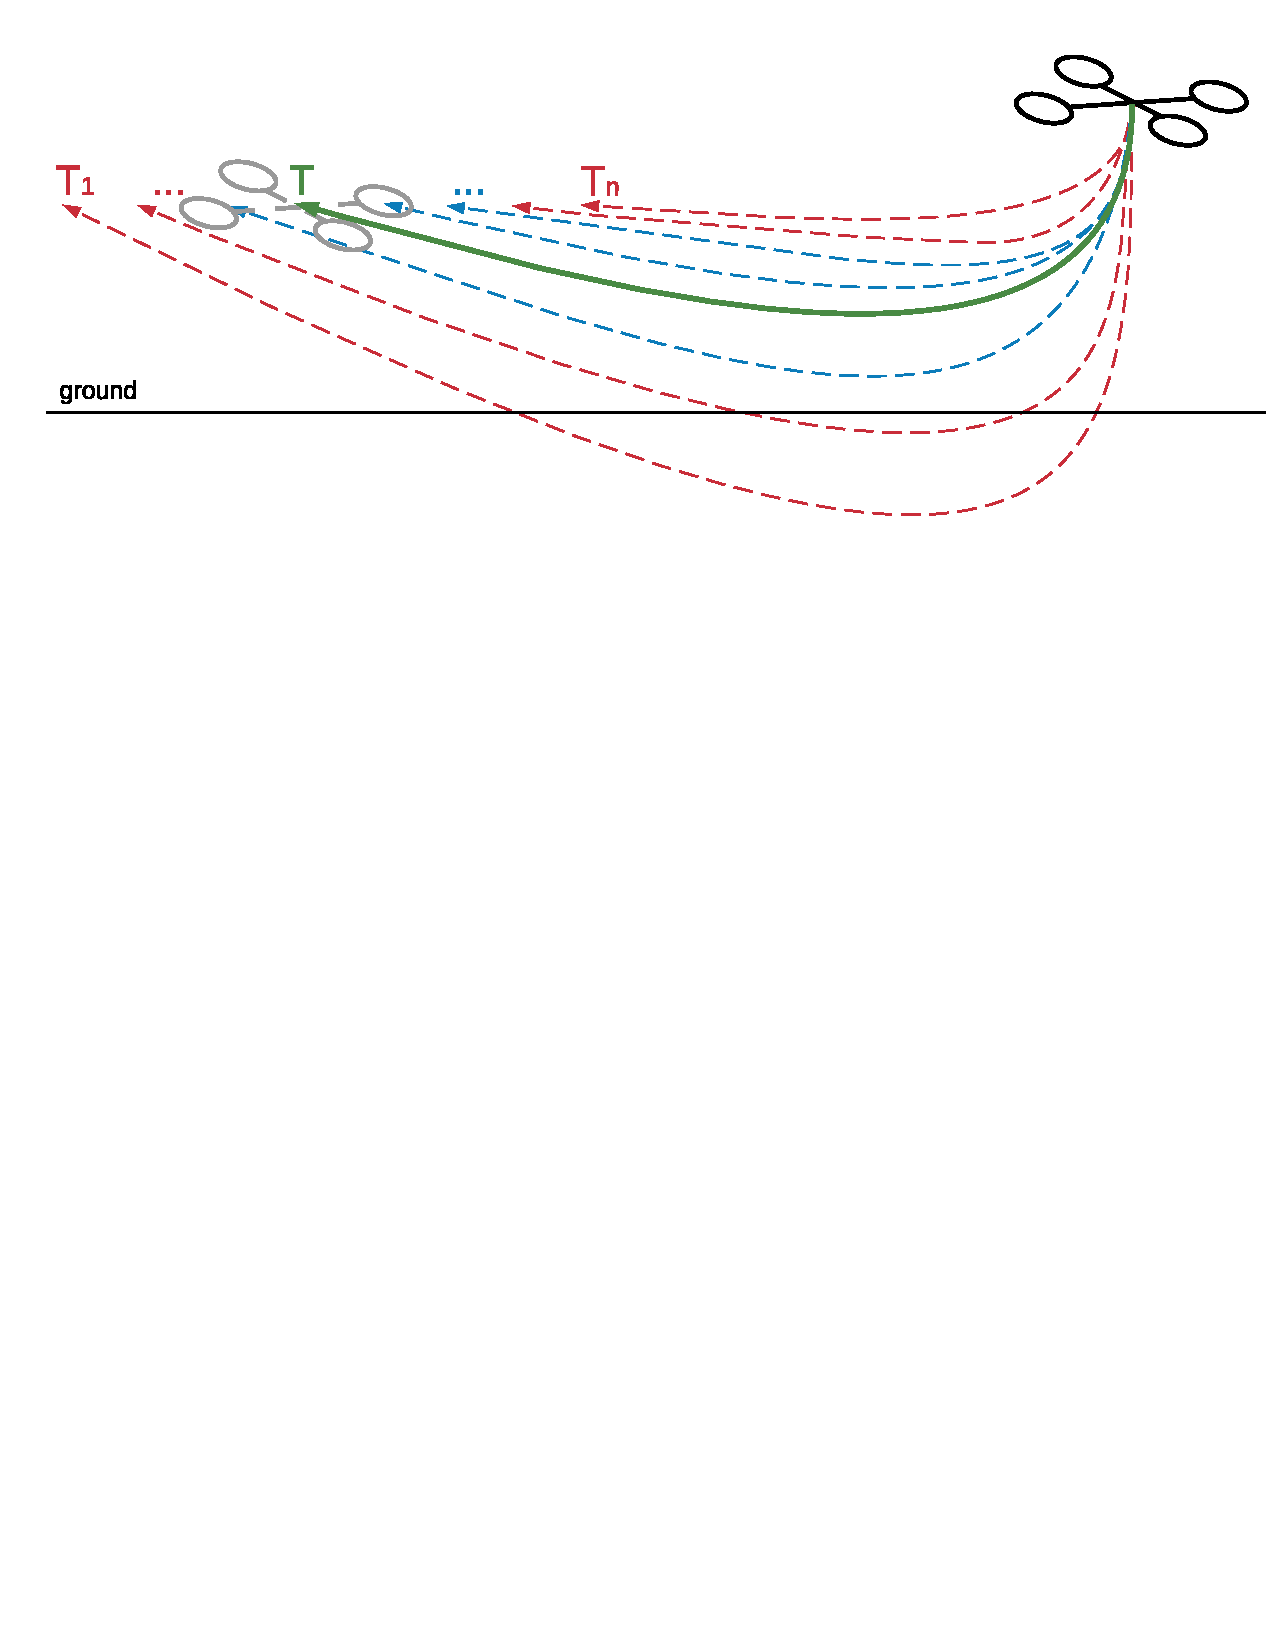
\includegraphics[width=0.8\textwidth]{img/trajectory_generation.pdf}
    \caption{The scheme synthesizes the concept of multiple possible trajectory generated and then pick the best one. The red trajectory are unfeasible (state or input unfeasible), the green trajectory is the best solution found.}
    \label{fig:traject_gen}
\end{figure}

The trajectory planning module is constituted by two threads:
\begin{itemize}
\item The first thread is popping and publishing the top of a stack of desired states with rate $r_{trj}$. This state will be the input of the high controller module.
\item The second thread:
\begin{itemize}
\item receives the initial and final conditions;
\item checks if these two belong to the previous trajectory (within an error), and only if they do not, proceed with the following tasks;
\item calculates the best trajectory;
\item samples the trajectory with a given rate $r_{trj}$;
\item substitutes the desired states inside the stack of the first thread with the new samples.
\end{itemize}
\end{itemize}

\begin{figure}[!htbp]
    \centering
    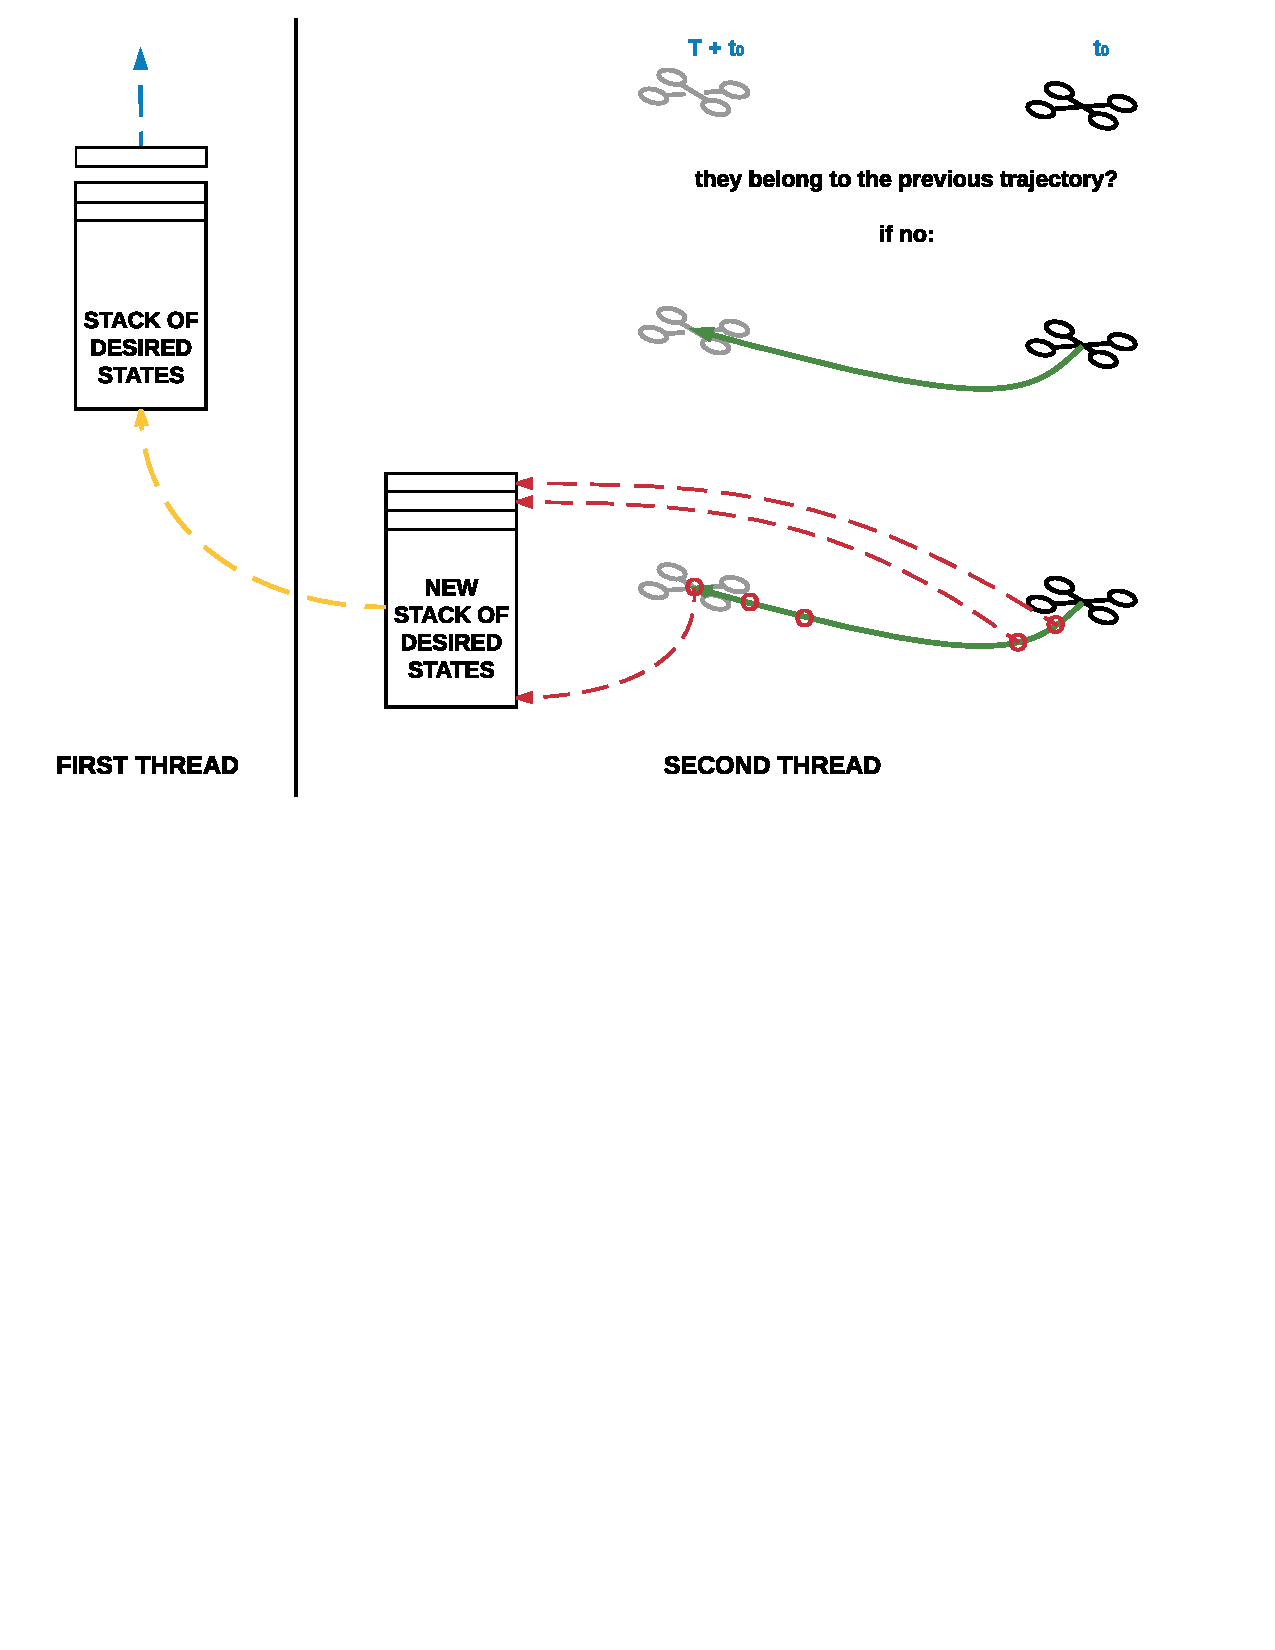
\includegraphics[width=1.0\textwidth]{img/threads_trajectory_generation.pdf}
    \caption{Scheme of tasks subdivision between the two threads.}
    \label{fig:traject_gen}
\end{figure}

In this module, we utilize the trajectory planning approach described in \cite{mueller2015computationally} to generate thousands of trajectories per second (\SI{2}{\milli \second} each), and then choose the best one to follow. We do this calculation with frequent replanning in order to correct any errors related to the prediction of the final target or related to a displacement between desired state and actual state of the quadrotor, due to the not perfect tracking of the trajectory by the controller.\\

\section{Minimum jerk trajectory}
The algorithm proposed in \cite{mueller2015computationally} produces trajectories that are the result of an optimal control problem with the goal of computing a thrice differentiable trajectory which guides the quadrotor from an initial state (position, velocity, acceleration and yaw of the UAV) to a final state in a finite time $T$, while minimizing a cost function that can be considered as an upper bound on the average of a product of the inputs to the quadrotor system.\\ Furthermore, the final trajectory takes in account feasibility with respect to input and space constraints.
\subsection{Dynamic Model}
Consider the classic simplified dynamic model of the quadrotor:
\begin{align}
\begin{cases}
\ddot{\boldsymbol{r}} = \boldsymbol{g} + \boldsymbol{R}_{WB}\boldsymbol{c}  \\[10pt]
\dot{\boldsymbol{R}}_{WB} = \boldsymbol{R}_{WB}\hat{\boldsymbol{w}_{WB}}
\end{cases},
\label{eq:dynamic_jerk}
\end{align}
where 
\begin{align}
\hat{\boldsymbol{w}_{WB}} =
{\begin{bmatrix}
0 & -\omega_3 & \omega_2 \\[10pt]
\omega_3 & 0 & -\omega_1 \\[10pt]
-\omega_2 & \omega_1  & 0
\end{bmatrix}} \ \ \ \ \ \ \boldsymbol{c} = 
{\begin{bmatrix}
0 \\[10pt]
0 \\[10pt]
c
\end{bmatrix}} = \boldsymbol{e}_3c.
\label{eq:52}
\end{align}
In \eqref{eq:52} input are  $c$, the total normalized thrust, and the angular rates $\omega_1,\omega_2,\omega_3$. Now the goal is to express these inputs in function of the states and the jerk.
 
The input thrust $c$ is computed by applying the norm to the position dynamics:
\begin{align}
c^2 &= ||\boldsymbol{c}||^2 =  ||\ddot{\boldsymbol{r}} - \boldsymbol{g}||^2, \\[20pt] \label{eq:thrust_from_jerk}
\begin{split}
2c\dot{c} &= 2(\ddot{\boldsymbol{r}} - \boldsymbol{g})^T \boldsymbol{j} = 2 c\boldsymbol{e}_3^T\boldsymbol{R}_{WB}^T \boldsymbol{j}  , \\[10pt]
\dot{c} &= \boldsymbol{e}_3^T\boldsymbol{R}_{WB}^T \boldsymbol{j} .
\end{split}
\end{align}

We can also define the position dynamics in therms of jerk:
\begin{align}
\boldsymbol{j} &= \dddot{\boldsymbol{r}} = \dot{\boldsymbol{R}}_{WB}\boldsymbol{c} + \boldsymbol{R}_{WB}\dot{\boldsymbol{c}}.
\end{align}

Combining the two derivations, we can say that fixed $\boldsymbol{j}$ and $c$, we define uniquely two components of the body rates:
\begin{align}
{\begin{bmatrix}
\omega_1 \\[10pt]
\omega_2
\end{bmatrix}}  = \frac{1}{c}
{\begin{bmatrix}
1 & 0 & 0  \\[10pt]
0 & 1 & 0
\end{bmatrix}}\boldsymbol{R}_{WB}^T \boldsymbol{j}
\label{eq:omega_from_jerk}
\end{align}
Using these equations the inputs of the system are defined with a degree of freedom in $\omega_3$.\\

The goal of this algorithm is to find  the trajectory $\boldsymbol{z}(t)$ for $t \in [0,T]$, consisting of the quadrotor position, velocity and acceleration, such that:
\begin{align}
\boldsymbol{z}(t) = (\boldsymbol{r}(t),\dot{\boldsymbol{r}}(t),\ddot{\boldsymbol{r}}(t)) \in \mathbb{R}^9
\end{align}
with given initial and final conditions $\boldsymbol{z}(0)$ and $\boldsymbol{z}(T)$.

If we consider the system input to be the three-dimensional jerk, then we can decouple the dynamics into three orthogonal inertial axes, and treat each axis as a triple integrator with jerk used as control input. The true control inputs $c$ and $\boldsymbol{\omega}$ are then recovered from $\boldsymbol{j}$  using \eqref{eq:thrust_from_jerk} and \eqref{eq:omega_from_jerk}.


\subsection{Optimal control problem}
The trajectory generation is rewritten as a discrete optimal control problem, with boundary conditions defined by the quadrotor initial and (desired) final states. The solution of this problem must minimize a cost function subject to some dynamics and satisfying state and inputs conditions.\\

As we said, the dynamics are split among the three decoupled axis, and for each axis the optimal control problem is  solved independently. For a single axis the problem is defined as follows. Find the sequence of control input $j_k$ that minimizes:
\begin{align}
J = \sum_{k=0}^{N-1} j_k^2,
\end{align}

subject to the dynamics:
\begin{align}
\begin{split}
j_k &= \dddot{r}_k,\\[10pt]
z_k  &= 
{\begin{bmatrix}
 r_k \\[5pt]
 \dot{r}_k \\[5pt]
 \ddot{r}_k
\end{bmatrix}} = 
{\begin{bmatrix}
1 & dt & \frac{dt^2}{2}  \\[5pt]
0 & 1 & dt \\[5pt]
0 & 0 & 1
\end{bmatrix}}z_{k-1} + 
{\begin{bmatrix}
 \frac{dt^3}{6}  \\[5pt]
 \frac{dt^2}{2} \\[5pt]
 dt
\end{bmatrix}}j_{k-1}, \\[10pt]
z_0 &= z(0), \\[5pt]
z_N &= z(T),
\end{split}
\end{align}
and respecting the constraints:
\begin{align}
A
{\begin{bmatrix}
 r_k \\[10pt]
j_k
\end{bmatrix}} \leq b.
\end{align}

The solution of this optimal control problem can be found in close form with Pontryagin's minimum principle.
In the paper \cite{mueller2015computationally} are presented all the calculations to derive the solution. The final result requires the evaluation of a single matrix that depends on the initial and final condition $z(0)$ $z(T)$ and the total time $T$.

\subsection{Cost function}
The cost function selected is, considering the three axis together:
\begin{align}
J = \sum_{k=0}^{N-1} ||\boldsymbol{j}_k||^2
\end{align}

This cost function has been chosen because it can be interpreted as an upper bound for a product of the input (using \eqref{eq:omega_from_jerk}):
\begin{align}
c_k^2||\boldsymbol{\omega}_k||^2 = \Big|\Big| c_k
\begin{bmatrix}
\omega_{1,k} \\[2pt]
\omega_{2,k}
\end{bmatrix}\Big|\Big|^2 = \Big|\Big| c_k \frac{1}{c_k}
{\begin{bmatrix}
1 & 0 & 0  \\[2pt]
0 & 1 & 0
\end{bmatrix}}\boldsymbol{R}_{WB,k}^T \boldsymbol{j}_k\Big|\Big|^2 \leq ||\boldsymbol{j}_k||^2
\end{align}

\subsection{Constraints}
The trajectory is feasible if $c$ and $||\boldsymbol{\omega}||$ respect the following conditions for all t of the trajectory:
\begin{align}
\begin{split}
0 < c_{min} \leq c &\leq c_{max},\\
||\boldsymbol{\omega}|| & \leq \omega_{max}.
\end{split}
\end{align}

These constraints can be rewritten in therm of the state and the jerk. For the thrust
\begin{align}
\begin{split}
 c_{min}^2 \leq c^2 &\leq c_{max}^2,\\
 c_{min}^2 \leq ||\ddot{\boldsymbol{r}} - \boldsymbol{g}||^2 &\leq c_{max}^2.\\
\end{split}
\label{eq:feasib_thrust}
\end{align}
For the body rates:
\begin{align}
\begin{split}
||\boldsymbol{\omega}|| =
 {\begin{bmatrix}
\omega_1 & \omega_2
\end{bmatrix}}
 {\begin{bmatrix}
\omega_1 \\[10pt]
\omega_2
\end{bmatrix}} + \omega_3^2 = {\begin{bmatrix}
\omega_1 & \omega_2
\end{bmatrix}}
 {\begin{bmatrix}
\omega_1 \\[10pt]
\omega_2
\end{bmatrix}}  \leq \frac{1}{c}||\boldsymbol{j}||  \leq \omega_{max} 
\end{split}
\label{eq:feasib_bodyrates}
\end{align}
where we assume $\omega_3 = 0$

\subsection{Feasibility check} \label{feasibility_check}
A fast conservative verification is applied to check the feasibility of the trajectory. For the thrust, from \eqref{eq:feasib_thrust}, we know that the trajectory is unfeasible if:
\begin{align}
\max_{k=[0,N]} {(\ddot{r}_{i,k}- \delta_{i,z}g)^2} > c_{max}^2 \ \ \ \ \forall i\in\{x,y,z\}, \\
\min_{k=[0,N]} {(\ddot{r}_{i,k} -\delta_{i,z}g)^2} < c_{min}^2 \ \ \ \ \forall i\in\{x,y,z\},
\end{align}
where $\delta_{i,z}$ is equal to $1$ if $i=z$ (we are considering the $z$ axis) otherwise it is $0$.\\
On the other hand the trajectory is definitely feasible if:
\begin{align}
\sum_i{\max_{k=[0,N]} {(\ddot{r}_{i,k}-  \delta_{i,z}g)^2}} \leq c_{max}^2 \ \ \ \ i\in\{x,y,z\},\\
\sum_i{\min_{k=[0,N]} {(\ddot{r}_{i,k} -  \delta_{i,z}g)^2}} \geq c_{min}^2 \ \ \ \  i\in\{x,y,z\}.
\label{eq:thrust_minmax}
\end{align}
If both these checks fail, the trajectory is considered interminable.\\

For the body rates, from \eqref{eq:feasib_bodyrates} we know that the trajectory is feasible only if:
\begin{align}
\ddfrac{\sum\limits_{i=1} \  \max\limits_{k=[0,N]} j_{i,k}^2 }{\sum\limits_{i=1} \ {\min\limits_{k=[0,N]} {(\ddot{r}_{i,k} -  \delta_{i,z}g)^2}}} \leq \omega_{max} \ \ \ \ i\in\{x,y,z\}
\label{eq:body_rates_max}
\end{align}

If the trajectory is indeterminable, then the feasibility checks are repeated separately in the two sub intervals $[1,\frac{N}{2}], [\frac{N}{2}+1,N]$, iteratively. The check stops when all the subset are feasible, or one is unfesible, or if the subdivision has arrived at intervals smaller than a certain threshold.


\subsection{Estimating the acceleration} \label{subsec:acceleration}
The trajectory generation method we used in this work needs an initial and a final state. The initial state is always selected as the current position velocity and acceleration of the quadrotor. From the state estimate of MSF we have the first two information, while the third has to be estimated separately.\\
There are several ways to obtain this estimate:
\begin{itemize}
\item IMU: the Inertial unit gives measurements of the 3D linear accelerations of the vehicle. This measures are noisy when the quadrotor is flying because of the motors vibrations. This renders necessary to filter the measure with a low pass:
 \begin{align}
a_{imu}(t_k) = \Big(1-e^{-\frac{t_k-t_{k-1}}{\tau_{a_{imu}}}}\Big)imu(t_k) + e^{-\frac{t_k-t_{k-1}}{\tau_{imu}}} a_{imu}(t_{k-1}).
\label{eq:imu_acc}
\end{align}
\item Finite difference: Having two successive velocity estimation we can calculate the acceleration approximating the derivative of the velocity with a numerical finite difference:
\begin{align}
\dot{v}(t_k) \simeq \frac{v(t_k)-v(t_{k-1})}{t_k-t_{k-1}},
\label{eq:finite_difference}
\end{align}
Also this method is really sensitive to high frequency noise, and the data must be filter with low pass filter:
 \begin{align}
a_{fd}(t_k) =  \Big(1-e^{-\frac{t_k-t_{k-1}}{\tau_{fd}}}\Big)\frac{v(t_k)-v(t_{k-1})}{t_k-t_{k-1}} + e^{-\frac{t_k-t_{k-1}}{\tau_{a_{fd}}}}. a_fd(t_{k-1})
\label{eq:finite_difference}
\end{align}
\item Thrust: from the equation of motion of the quadrotor we know that the acceleration of the UAV in a specific moment is completely described by the total thrust $\boldsymbol{c}$ applied and the rotation of the quadrotor $\boldsymbol{R}_{WB}$ :
\begin{align}
{\begin{bmatrix}
\ddot{x} \\[10pt]
\ddot{y} \\[10pt]
\ddot{z}
\end{bmatrix}}=
{\begin{bmatrix}
0 \\[10pt]
0 \\[10pt]
-g
\end{bmatrix}} 
+ \boldsymbol{R}_{WB}
{\begin{bmatrix}
0 \\[10pt]
0 \\[10pt]
c
\end{bmatrix}}.
\end{align}
Also, we know that:
 \begin{align}
c = \frac{1}{m}\sum_{i=1}^{4}{f_i},
\end{align}
where $f_i$ is the thrust produced by the $i$-th propeller.\\
From the low level controller Eq~\eqref{eq:thrusts} we have these values, and so we can calculate the acceleration vector. It is important to notice that the information from the low level control are the desired thrust for each propeller $\tilde{f}_i$, not the actual one $f_i$. The real produced thrust can be calculated as $\lambda_i\tilde{f}_i$ where $\lambda_i$ is the rotor fitness coefficients. These coefficients are estimated in hover conditions before starting the mission.
\end{itemize}

In the final implementation we decided to use the thrust that, even if it shows some offset in the z direction (see Sec.~\ref{subsec:acceleration_experiments} for more details) with respect to the other two methods, is more smooth and does not need a filtering.


\section{Minimum snap trajectory}
When the minimum snap trajectory algorithm fails to find a feasible trajectory, and no previous trajectories are available, we have to find another way to calculate the sequence of desired states.\\
If this is the case, we use a minimum snap trajectory \cite{mellinger2011minimum}. This type of trajectories are the solution of another optimization problem in which the inputs are expressed in function of the fourth derivative of the position, namely the snap.\\

The problem formulation uses a more complete dynamics of the quad with respect to the jerk formulation \eqref{eq:dynamic_jerk}
:
\begin{align}
\begin{cases}
\ddot{\boldsymbol{r}} = \boldsymbol{g} + \boldsymbol{R}_{WB}\boldsymbol{c}  \\[10pt]
\dot{\boldsymbol{R}}_{WB} = \boldsymbol{R}_{WB}\hat{\boldsymbol{w}_{WB}}  \\[10pt]
\dot{\boldsymbol{w}}_{WB} = J^{-1} (\boldsymbol{\tau} - \boldsymbol{w}_{WB} \times J\boldsymbol{w}_{WB})
\end{cases}
\end{align}
where $\boldsymbol{\tau}$ are the torques acting on the body causated by the totor thrust \eqref{eq:torques}.\\

Using these dynamics we need a derivative more in order to express the input in therms of the flat outputs.
Because of that, the states must be described as position, velocity, acceleration and jerk. \\
In order to compute this type of trajectory we should calculate the initial jerk, but since it is difficult to estimate its value we set the initial and final jerks to be zero, while the other values of the initial condition are calculated as the previous section's algorithm.\\

In this new formulation, the optimization problems minimizes the following cost function:
\begin{align}
J = \sum_{k=0}^N\Big( \mu_r \Big|\Big|\frac{d^{4}\boldsymbol{r}_k}{dt^{4}}\Big|\Big|  +  \mu_{\psi} \Big|\Big|\frac{d^{2}\boldsymbol{\psi}_k}{dt^{2}}\Big|\Big|\Big).
\end{align}
%that is minimizing the snap (because the thrust and pitch and roll body rates are expressed as functions of the forth derivative of the position $\boldsymbol{r}$), and the yaw angular acceleration for minimizing the input relative (in the paper  \cite{mellinger2011minimum} there are all the calculations to express the inputs as function of the snap).

Since this problem does not have a close form, it is written as a quadratic program:
\begin{align}
\begin{split}
min & \ \ \boldsymbol{x}^T\boldsymbol{H}\boldsymbol{x} + \boldsymbol{h}^T\boldsymbol{x},\\[10pt]
s.t. &\ \ \boldsymbol{Ax} \leq \boldsymbol{b}
\end{split}
\end{align}
and then solved with optimization algorithms, finding numerically the result.\\ 

This problem requires, on average, more time to be solved (\SI{20}{\milli \second}) with respect to the minimum jerk method, so it is not possible to generate multiple trajectories and select the best one at each control loop.\\

What we are do is calculating this trajectory taking, among all the final conditions that the state machine is given as input to this module, the one with longest time $T$ and so producing the trajectory of $T_{max}$ seconds from the initial state to this point, because, usually, the longer is the time $T$ the less aggressive must be the trajectory to reach the final state, so it is more probable that this trajectory we are calculating is feasible .

\section{Trajectory generation issues} \label{sec:trajectory_problem}
The trajectory generator previously described presents some issues that must be solved. In the following we report the main ones together with possible solutions.

\subsection{Last chance solution}
If both rapid trajectory and minimum snap trajectory do not find a feasible solution we apply this final method.\\

This method uses the rapid trajectory algorithm calculated with a final time $T_{feasible}$ such that the trajectory is surely feasible. In the paper \cite{mueller2015computationally} there is a method to calculate $T_{feasible}$ for a trajectory from rest to rest states (initial e final velocity and accelerations equal to 0).\\
In our case, the initial state can also be not static, so the solution should not hold in our case. What we can do is to enlarge the time $T_{feasible}$, from rest to rest, by a factor $\alpha$ proportional to the initial acceleration and velocity, and using this final time to calculate the rapid trajectory.\\

The minimum time $T_{feasible}$ is defined as the maximum between three different final times. The 3 times are calculate to guarantee the maxim thrust feasibility $T_{c_{max}}$, the minimum thrust feasibility $T_{c_{min}}$ and the body rates feasibility $T_{\omega_{max}}$. \\

We take 
\begin{align}
T_{feasible} = \alpha \max{(T_{c_{max}},T_{c_{min}},T_{\omega_{max}})},
\end{align}
because if  we calculate a feasible trajectory $trj_1$, from static to static states, with terminal time $T_1$, and then we calculate $trj_2$ with $T_2 \geq T_1$ as new terminal time, then the second trajectory will be surely feasible (this is not always true if initial and final conditions are not resting).\\

The parameters necessary to find these times are the distance $d$ between initial and final position, $c_{min}$, $c_{max}$ the minimum and maximum thrust, and $\omega_{max}$ the maximum body rates.\\ 
Substituting these variables into the general solution of the optimal control problem, calculating the maximum acceleration that the final trajectory will have, and using Eqs. \eqref{eq:thrust_minmax} and \eqref{eq:body_rates_max}, we can find the thee values of time:
\begin{align}
T_{c_{max}} &= \sqrt{\dfrac{10d}{\sqrt{3}(g-c_{min})}} \\[10pt]
T_{c_{min}} &= \sqrt{\ddfrac{10d}{\sqrt{3}(c_{max}-g)}} \\[10pt]
T_{\omega_{max}} &= \sqrt[3]{\ddfrac{60d}{\omega_{max}c_{min}}}
\end{align}

At this point, we can calculate the trajectory between the initial and final position with time duration $T_{feasible}$. This trajectory is considered a temporal solution, so as soon as a new initial or final condition arrive, we try to substitute it with a new trajectory. \\

Note that the solution found with this last method could not lead to the correct completion of the task in the last two parts of the state machine. In these phases the quadrotor must be in a precise amount of time $T$ in a specific position, in order to intersect the moving platform, while we are now considering a trajectory with duration $ T_{feasible} \neq T$.


%\subsection{Too frequent replanning}
%The main drawback of the algorithm used is that, in theory, it is possible to replan the trajectory at each control loop: in a MPC style, at each cycle, we calculate a trajectory from the initial state state to the final one and communicate just the first desired state to the high level control, repeating this procedure at the next loop.\\
%In practice, using this algorithm, the continuous replanning is not possible: when we pass the first desired state at the high controller the difference in position, velocity and acceleration are too tiny to actually generate a response from the quadrotor and start a movement. The outcome of this process is that the UAV does not move, as it should, and at the following control cycle the initial condition are only slightly changed, so the quadrotor results static in the initial position.\\
%
%This behaviour usually does not happen when we have to perform a trajectory in which the altitude is decreasing (small thrust required), but it is a great issue when the $z$ position should remain equal or increasing.\\
%This is why we do not perform a replan at each loop but only when it is necessary so when the final desired state has changed or the quadrotor is not tracking the trajectory.
%
%\begin{figure}[!htbp]
%    \centering
%    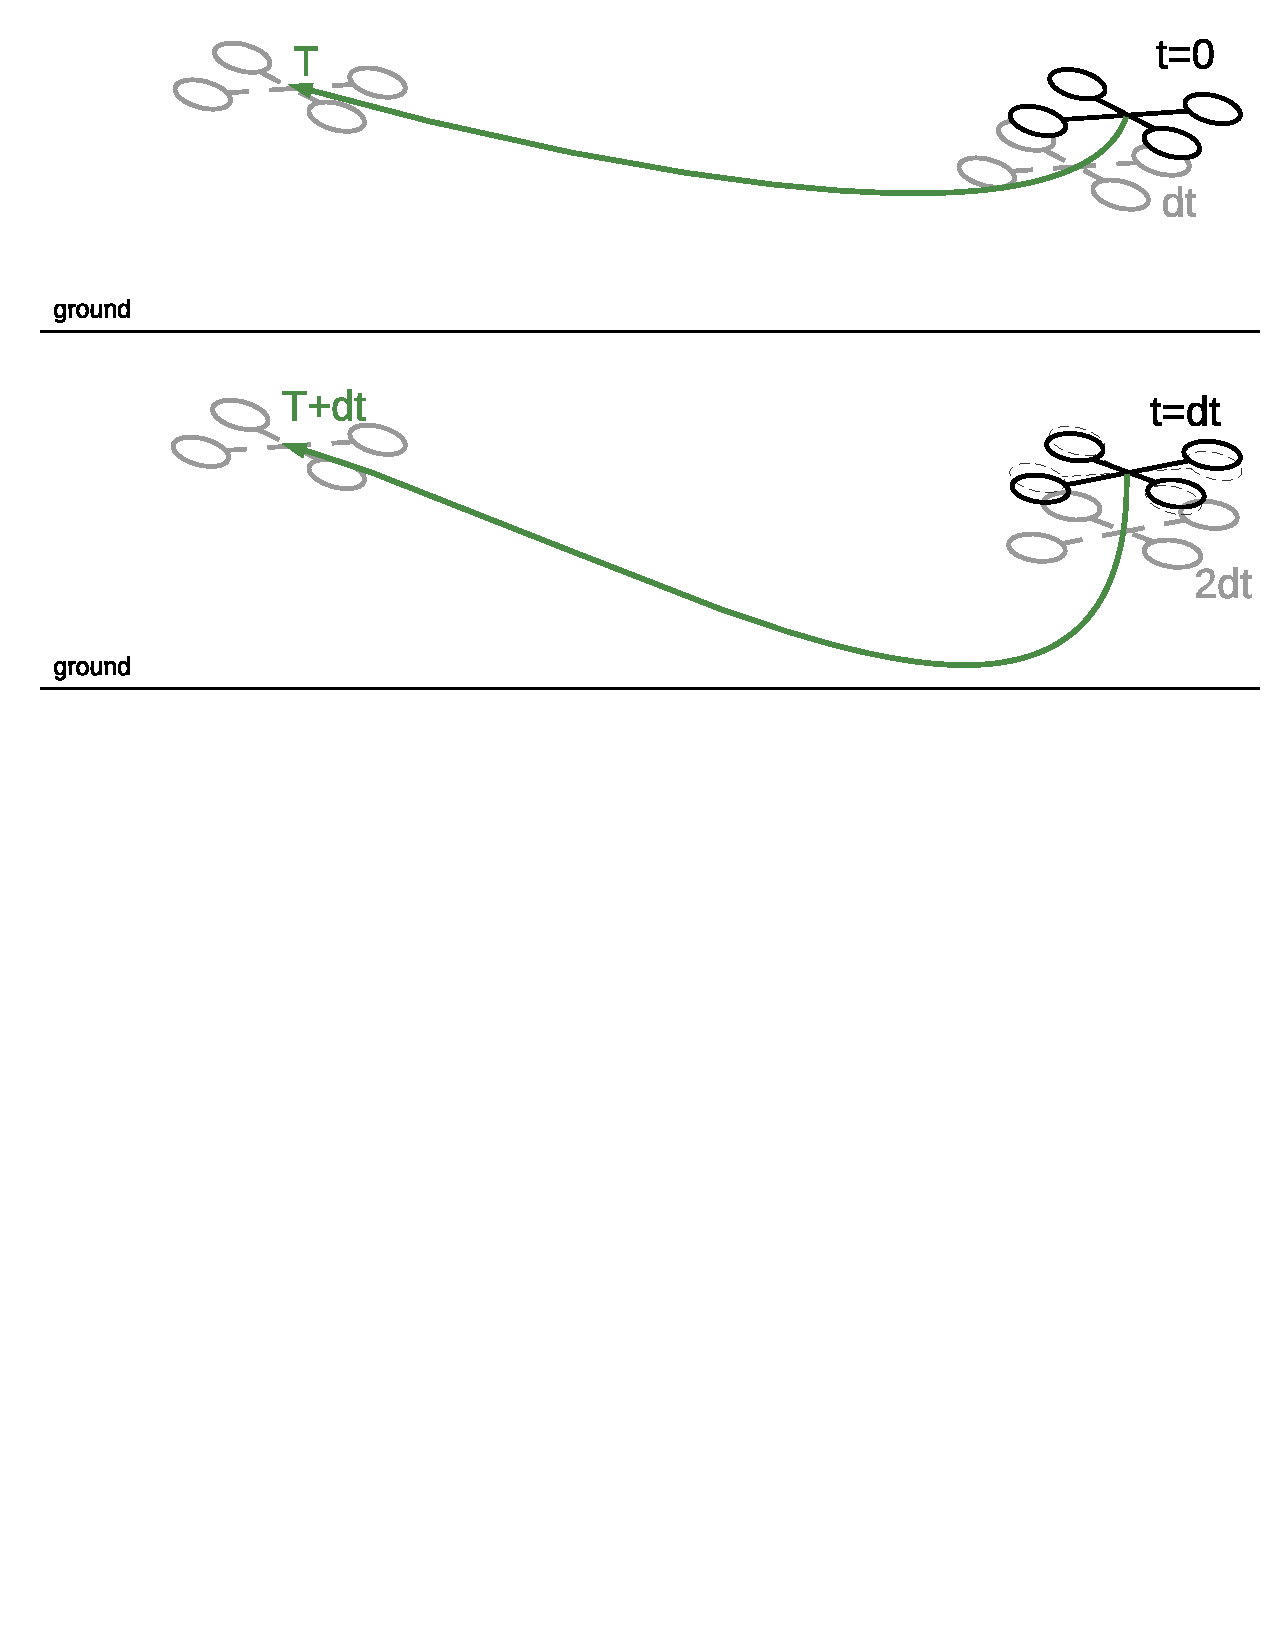
\includegraphics[width=0.7\textwidth]{img/frequent_replanning.pdf}
%    \caption{The scheme synthesizes the concept too frequent replanning. The quadrotor at time $dt$ should be in a position but the controller are not able to bring the UAV there. At the next loop the state of the quad is almost not changed, so it remains fixed in its initial state.}
%    \label{fig:freq_replan}
%\end{figure}


\subsection{Too short final time}
The rapid trajectory algorithm has another issue: when the final time $T$ is too short, all the calculated trajectories result indeterminable. This problem is due to the method used to check the feasibility with respect to the input, \ref{feasibility_check}, but to overcome this problem we can reduce the threshold for which the algorithm stop to recursively control if a piece of the trajectory is feasible.\\
This way the generation of the trajectory is slower, but we are able to find feasible trajectories when their duration is short.


%\chapter{Nonlinear Model Predictive Control}\label{chap:nonlinear_mpc}


\section{Model}

\section{Cost Function}

\section{Acado Library}


\section{Learning}


\section{Results}

\chapter{Experiments}\label{chap:experiments}
During this thesis, several experiments were performed in order to evaluate the performance of the framework.
We did different tests of all the parts of the modules, both in simulation and in the real world, in order to understand the weakness of each module and achieve better results.

In this chapter we describe the hardware used in the real world experiments and the software use for the simulations.
Finally, we report the main results achieved during these experiments.
%The system developed, utilize the Robot Operating System (ROS) [19]

\section{Real world hardware}
In all the real world experiments we use only onboard sensing and computing.
An OptiTrack motion-capture system \cite{optitrack} is used to have a ground truth values during some experiments, but the quadrotor never uses these data to fly.

\subsection{Quadrotor}
We utilize custom-designed quadrotors that are based on 3D printed and electronic parts designed in the RPG lab, combined with some commercial components (see Fig.~\ref{fig:quad_hardware}).

These platforms are lightweight (around \SI{500}{\gram}) and safe for operation in proximity with humans. However, they are also agile while maintaining maneuverability and robust vision-based control: they can achieve a maximum speed of at least \SI{4}{\meter \per \second} during vision-based flight.
The quadrotor used is equipped with:
\begin{itemize}
\item an IMU that provides linear accelerations and angular rates;
\item a quad-core single board computer (Odroid XU4), where all computations described in the previous chapters are performed;
\item two different cameras:
\begin{itemize}
\item a downward looking camera with a FoV of \SI{90}{\degree}, used to detect and track the moving platform;
\item a forward looking camera with fish-eye lens, used for state estimation. The fish-eye is used to have a wide field of view and be able to track enough features in every configuration.
\end{itemize}
\end{itemize}

\subsection{Moving platform}
During the experiments we use Jackal UGV as moving platform.\\ 
Jackal is a small field robotics research platform produced by Clearpath Robotics \cite{clearpathrobotics}. It has an onboard computer, GPS, IMU and it is fully integrated with ROS.\\
It can reach a maximum speed of \SI{2}{\meter \per \second}, that is perfect for testing with conditions similar to the final challenge.\\
Over the UGV we have installed a wooden base \SI{1}{\meter} $\times$ \SI{1}{\meter} were we attached both the textures in Fig.~\ref{fig:finalplatform} or the one in Fig.~\ref{fig:tempplatform}.

\begin{figure}[!ht]
    \centering
    \includegraphics[width=1.0\textwidth]{img/real_world_hardware.jpg}
    \caption{The UAV and UGV used during the experiments}
    \label{fig:quad_hardware}
\end{figure}


\section{Simulation}
A simulation environment is developed in order to recreate as precise as possible the final environment of the challenge.  As a matter of fact, organizing experiments in real field as large as the one in the challenge, can be difficult, but with the simulation environment we can test the whole framework before trying it in the real world.

The simulation is done using Gazebo simulator \cite{gazebosimulator}: it is a free simulation toolbox useful to reproduce populations of robots in complex indoor and outdoor environments, furthermore this toolbox is directly part of ROS.\\
To simulate the quadrotor we use the RotorS simulator \cite{rotors2016}: a UAV Gazebo simulator that provides some multirotor models among which there is the AscTec Hummingbird, very similar to the quadrotor we are using in the real world experiments. All quadrotors can be provided with many sensors such as IMU, cameras etc. \\
To simulate the moving platform we use the ROS package \cite{RobotsHusky} that allows us to control a Clearpath Husky. Over the UGV we installed a platform identical to the one used in the real world.\\

The framework used during the tests in the simulation are the same ones explained in Chap.~\ref{chap:general_framework}, with the difference that the state estimation is not coming from SVO+MSF, but is given by Gazebo and we corrupted it with a Gaussian noise with 0 mean and $\sigma^2$ variance.

\begin{figure}[!ht]
    \centering
    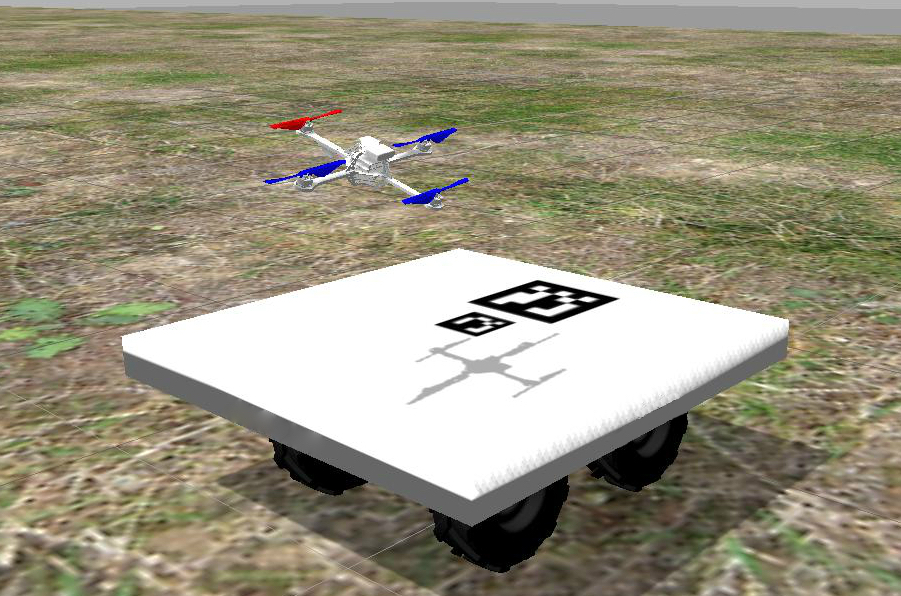
\includegraphics[width=1.0\textwidth]{img/simulation.jpg}
    \caption{The UAV and UGV used during the experiments in simulation}
    \label{fig:quad_ugv_sim}
\end{figure}

\section{SVO}
For this project we need to use a front looking camera for the visual odometry, because, when the UAV is over the base, the majority of the image from the down looking camera is occluded by the platform itself.\\
This is a crucial problem because the features on the base cannot be considered: the perceived movement is relative to the moving platform and not to the world frame. For example, in the scenario in which the quadrotor and the platform are moving with the same velocity, the images taken from the camera are not changing over time, even if the camera is moving. In this case the visual odometry fails to provide reliable results.\\
In the final parts of the mission, using the down looking camera, there will be not enough good features to track  for UAV state estimation, so is necessary to use a front looking camera for self state estimation.

\subsection{Front looking vs down looking}
To compare the results of front looking and down looking SVO we took datasets in which we run two instances of SVO (using the two different images from the two cameras) to compute the pose estimation of the quadrotor and then filter these pose with MSF using the same IMU signal. These state estimations are compared also with the ground truth from the OptiTrack. This way we can compare the two versions of SVO+MSF with the real pose.

The following images show the the results of one of these experiments. In this particular test we hold the quadrotor by hand and we move it inside the flyingroom simulating a square trajectory Fig.~\ref{fig:comparision_svo_trajectory}.

\begin{figure}[!htbp]
    \centering
    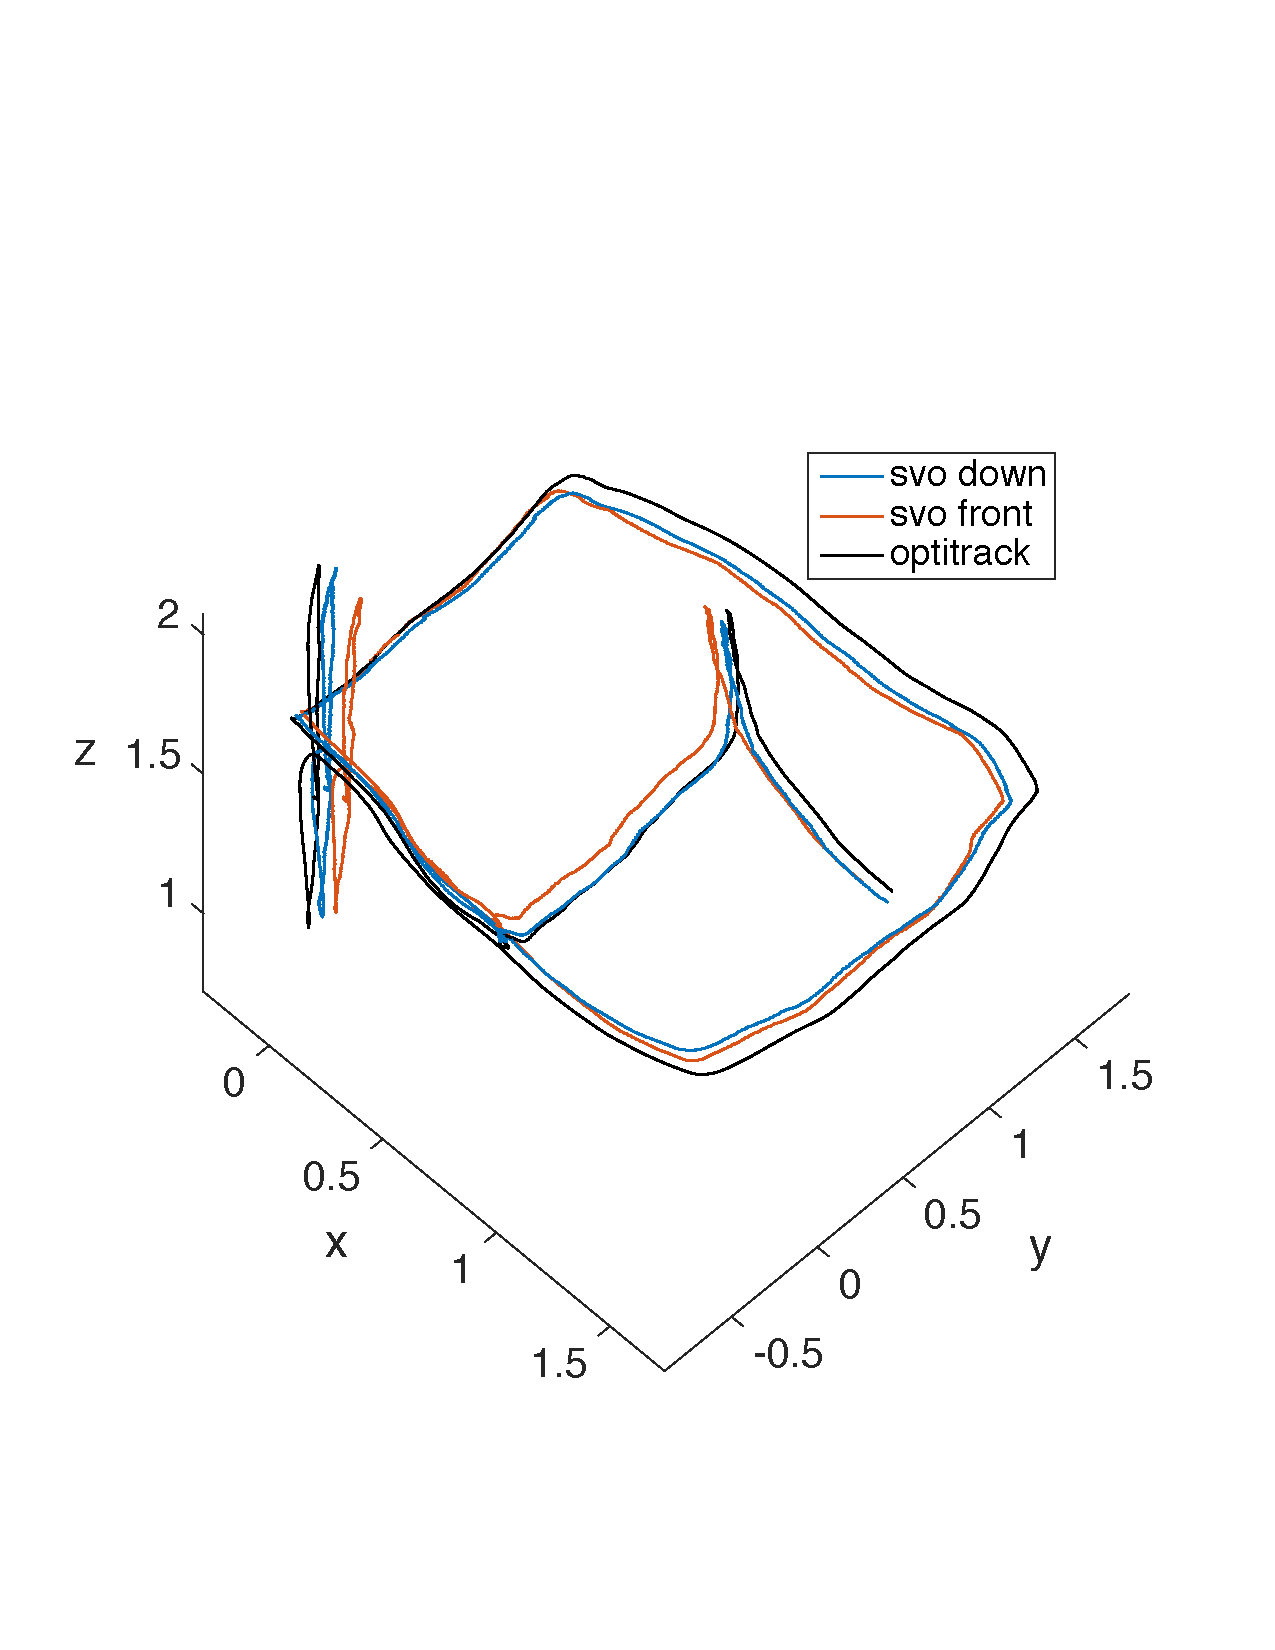
\includegraphics[width=0.9\textwidth]{img/comparision_between_two_svo_and_opti_trajectory.pdf}
    \caption{Comparison between SVO position estimation in 3D world. The blue line is the estimation with down looking camera, the red line with front looking one and the black line the ground truth given by the OptiTrack}
    \label{fig:comparision_svo_trajectory}
\end{figure}

In particular, Fig.~\ref{fig:comparision_svo_position} shows the position , Fig.~\ref{fig:comparision_svo_angles} the orientation and Fig.~\ref{fig:comparision_svo_velocities} the velocity estimations from the two versions of SVO compared to the OptiTrack.
 
\begin{figure}[!ht]
    \centering
    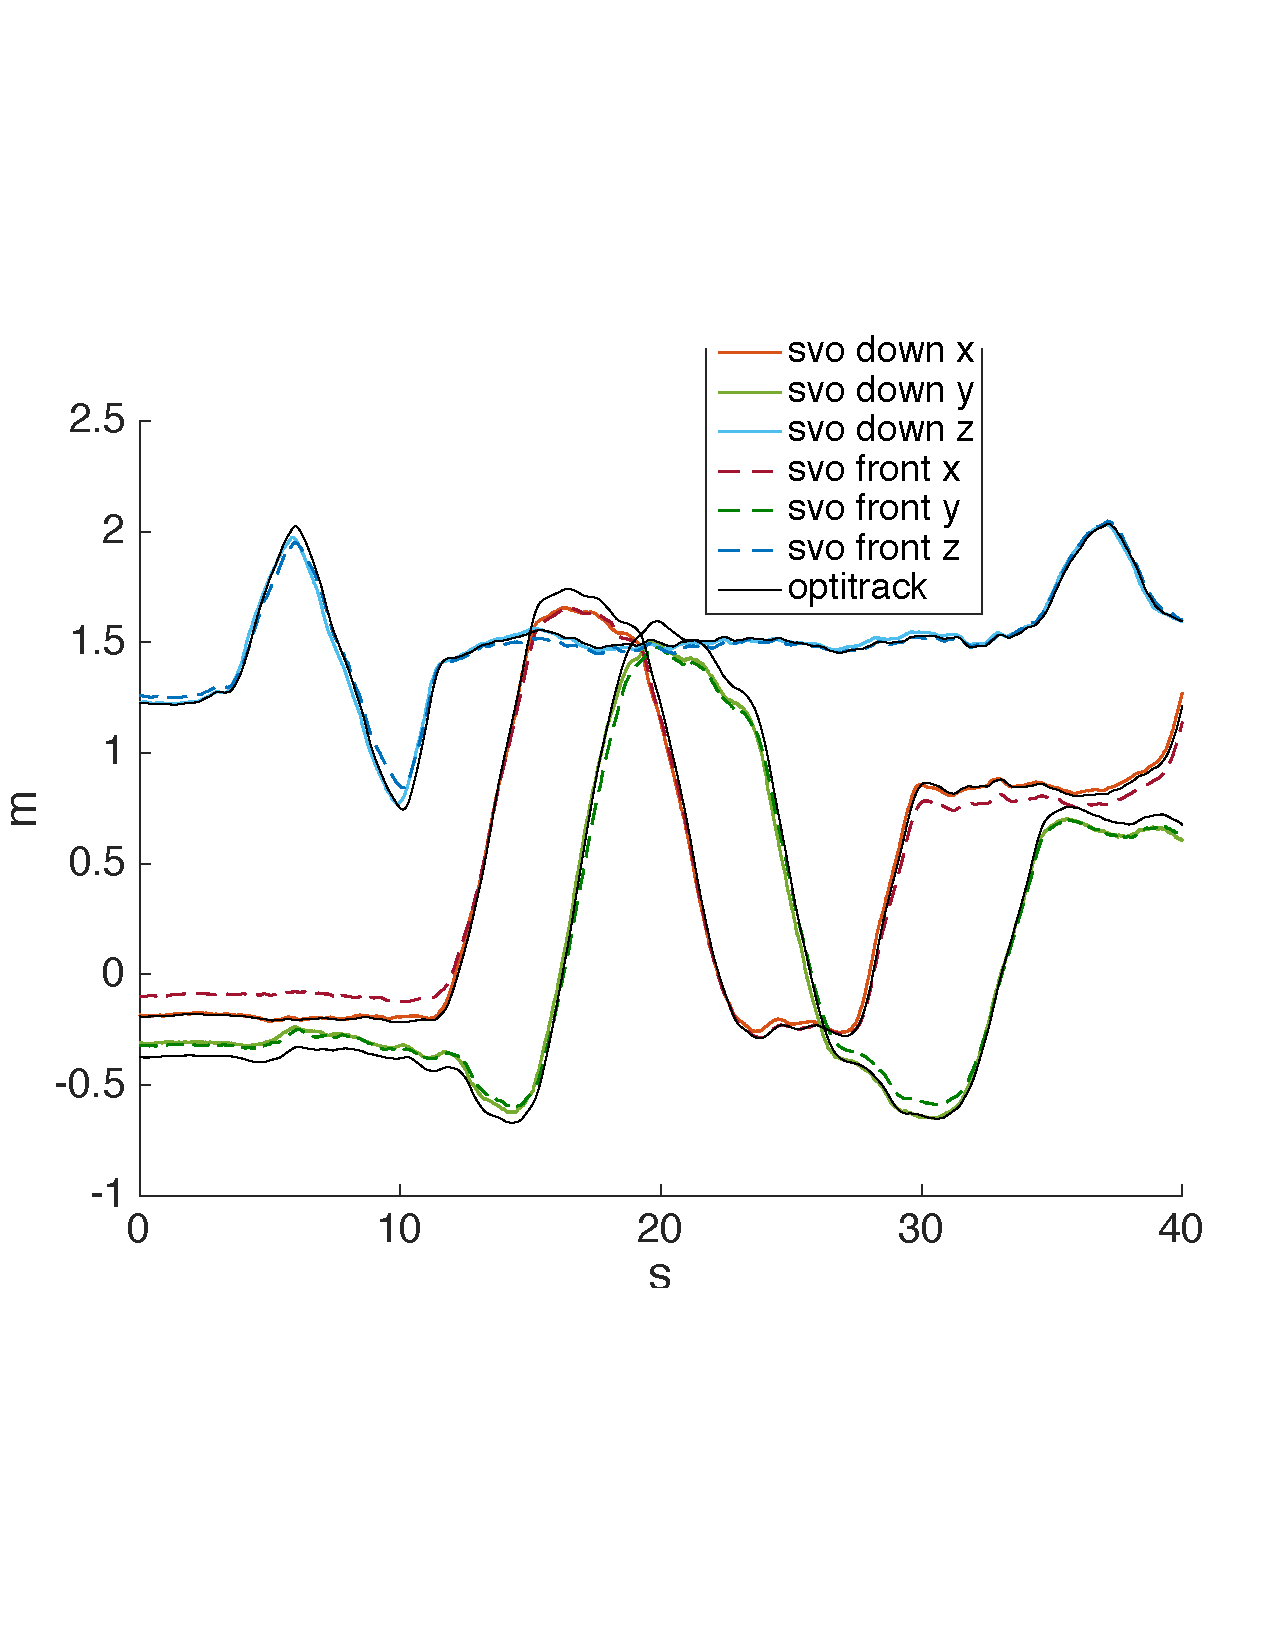
\includegraphics[width=0.8\textwidth]{img/comparision_between_two_svo_and_opti_position.pdf}
    \caption{Comparison between SVO position estimations with the front looking camera (dashed lines), down looking camera (solid) and optitrack (black).}
    \label{fig:comparision_svo_position}
\end{figure}

\begin{figure}[!ht]
    \centering
    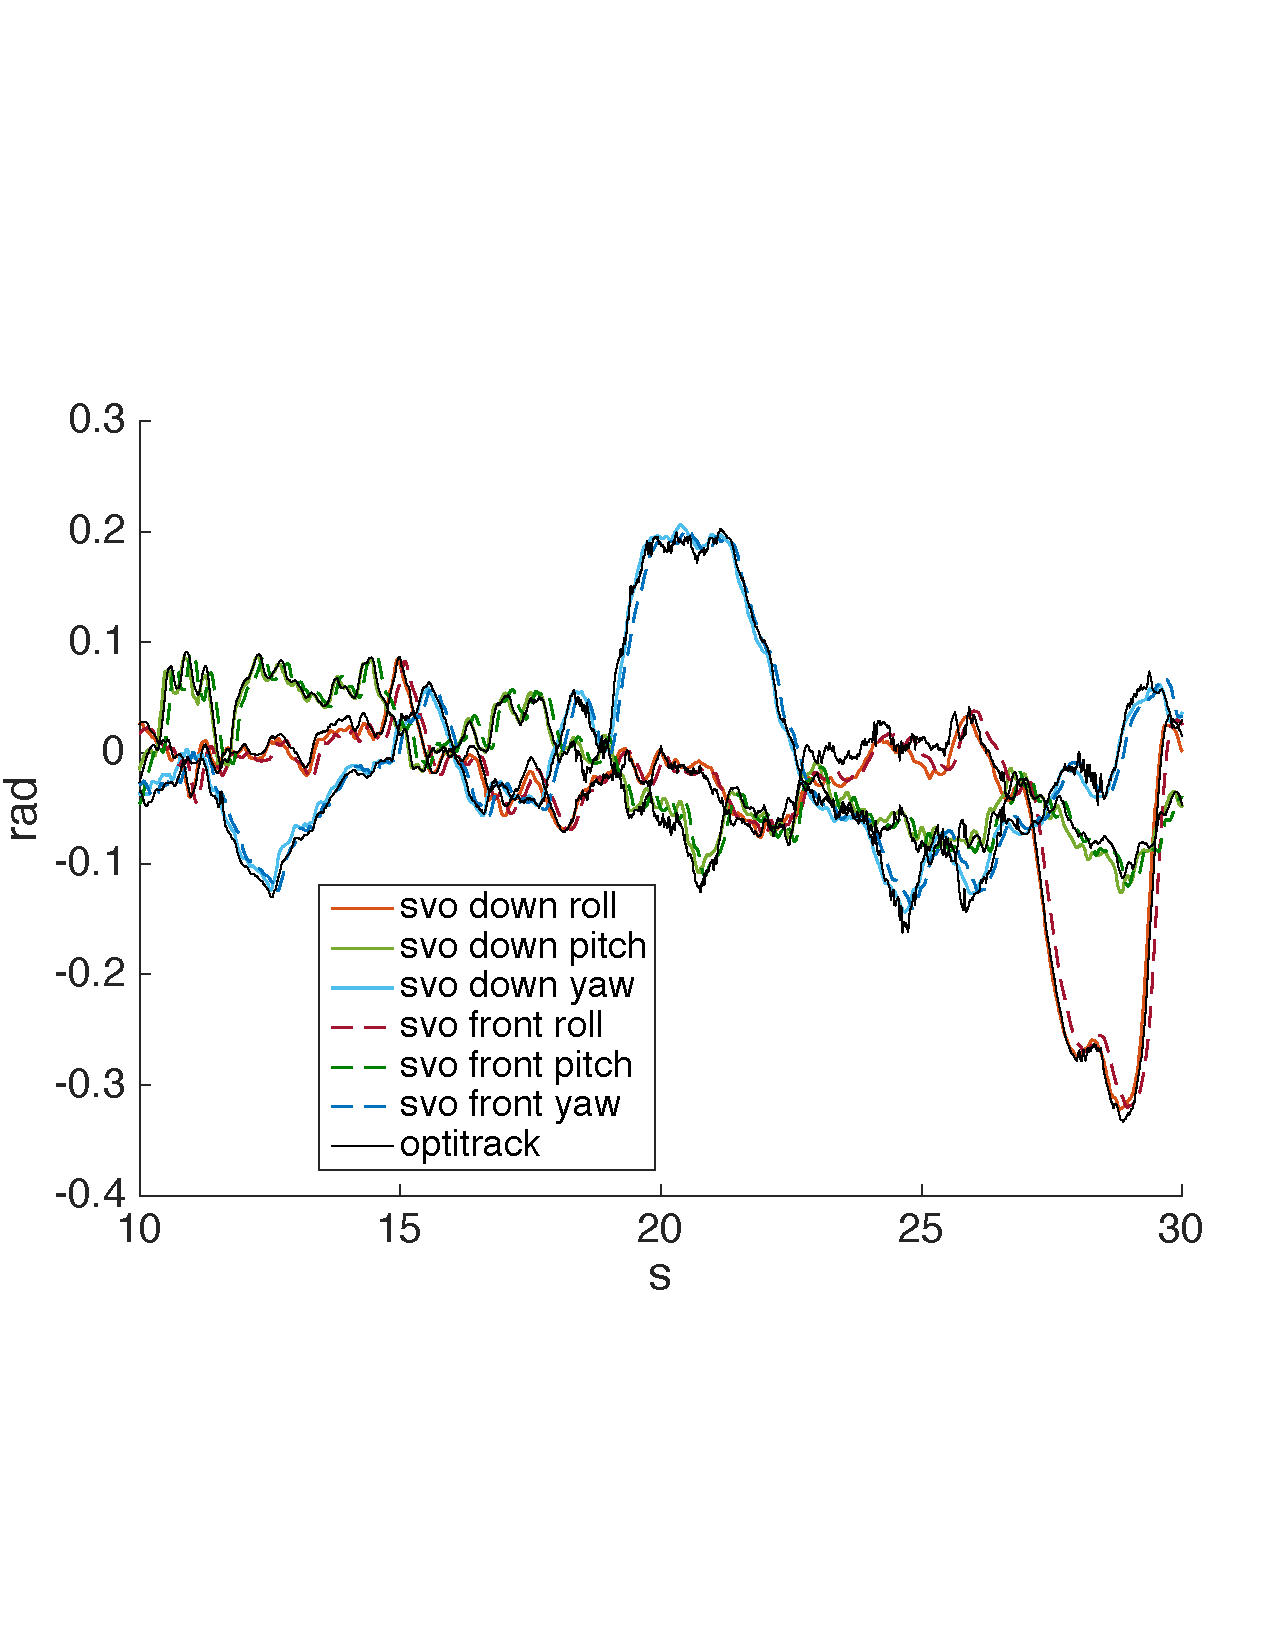
\includegraphics[width=0.8\textwidth]{img/comparision_between_two_svo_and_opti_angles.pdf}
    \caption{Comparison between SVO orientation estimations with the front looking camera (dashed lines), down looking camera (solid lines) , and OptiTrack (black lines). The orientation data from the OptiTrack are low pass filtered in order to eliminate the high frequency noise.}
    \label{fig:comparision_svo_angles}
\end{figure}

\begin{figure}[!ht]
    \centering
    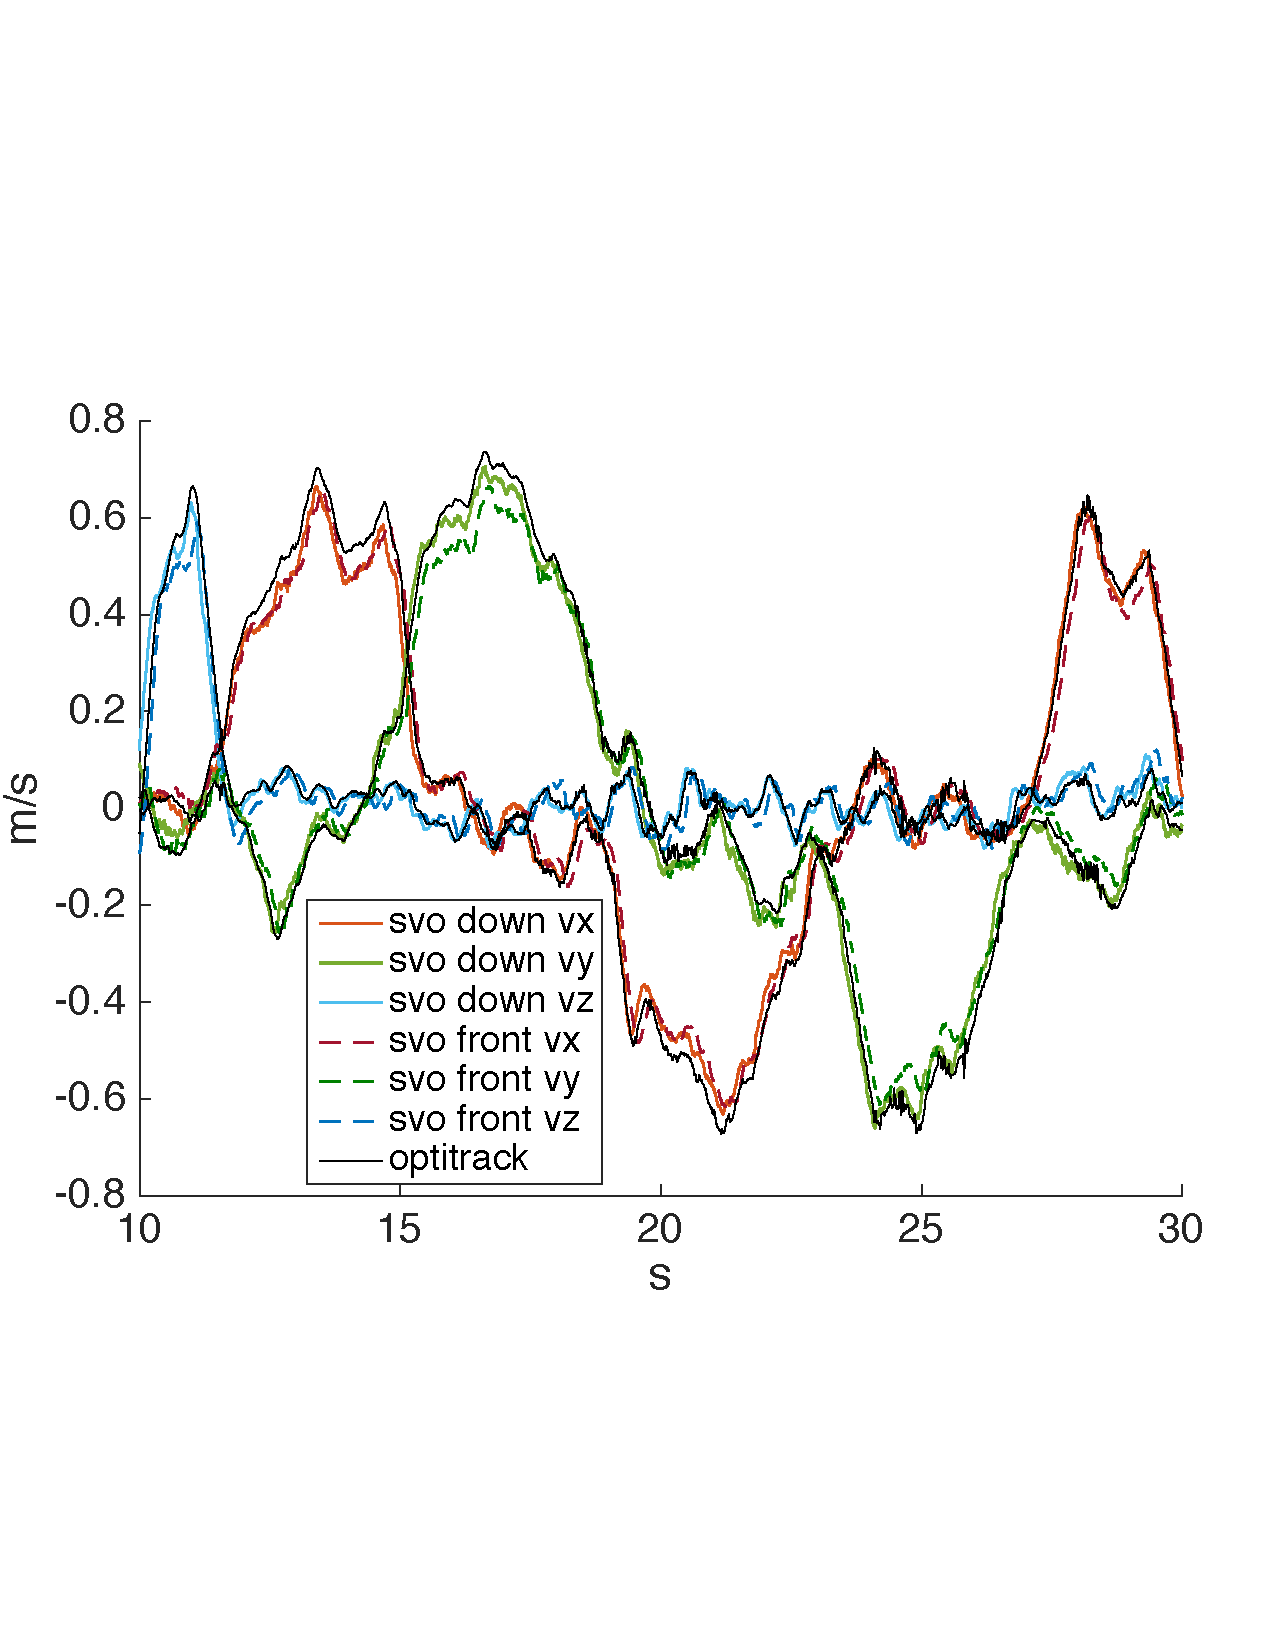
\includegraphics[width=0.8\textwidth]{img/comparision_between_two_svo_and_opti_velocities.pdf}
    \caption{Comparison between SVO position estimations with the front looking camera (dashed lines), down looking camera (solid lines), and OptiTrack (black lines). The velocity data from the OptiTrack are low pass filtered in order to eliminate the high frequency noise. }
    \label{fig:comparision_svo_velocities}
\end{figure}

We can see that both versions of our estimation framework provide a reliable estimation of the quadrotor pose and velocity. In order to evaluate the precision of the two estimations, see Fig.~\ref{fig:comparision_svo_error}, where the average position error between the two versions of SVO is shown: error generally below \SI{10}{\centi \meter} with RMSE of \SI{4.5}{\centi \meter} for the down looking camera and \SI{6}{\centi \meter} for the front looking one.\\

\begin{figure}[!ht]
    \centering
    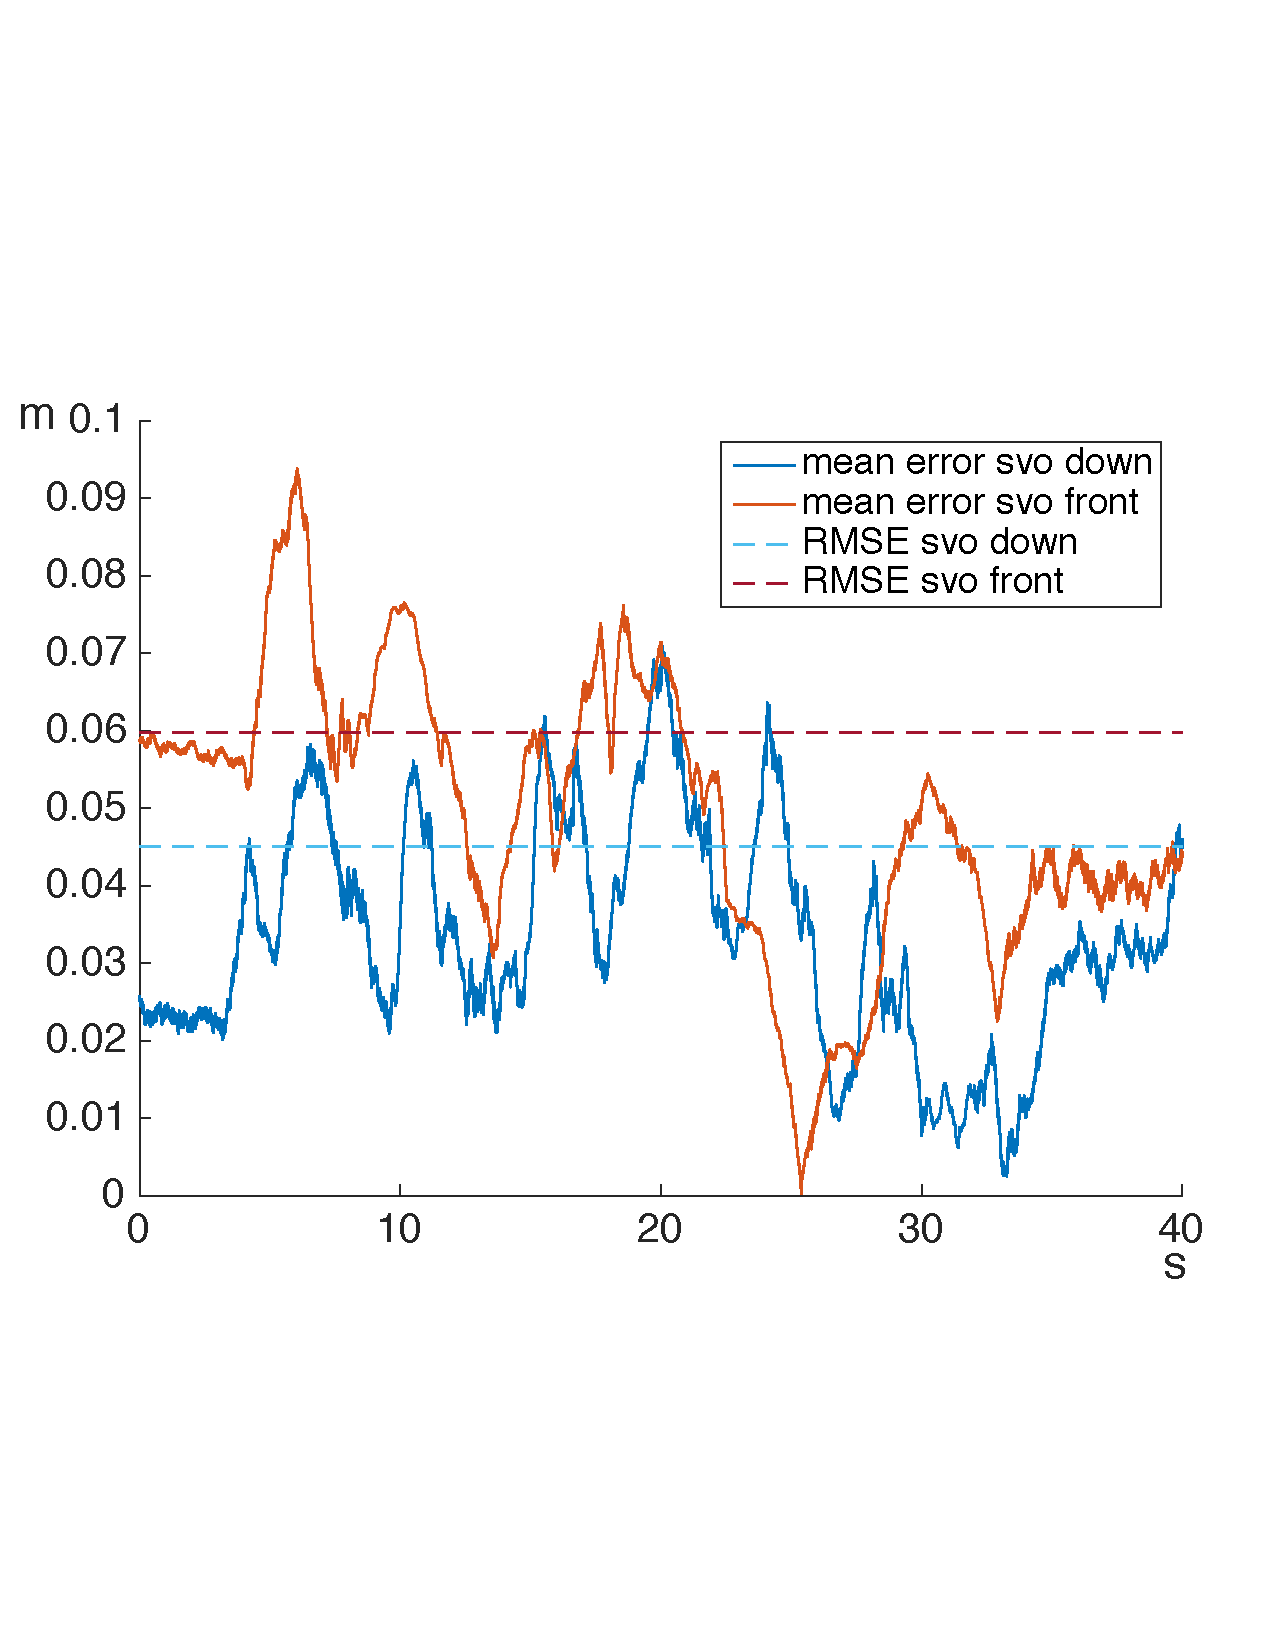
\includegraphics[width=0.9\textwidth]{img/comparision_between_two_svo_and_opti_error.pdf}
    \caption{Mean error between the 3D position estimations of the two versions of SVO and the ground truth. Blue line is the error with the down looking camera, the red line with the front looking one. The correspondent dashed lines are the RMSE for the two estimations.}
    \label{fig:comparision_svo_error}
\end{figure}

%This error is larger then expected. In particular the graphs \ref{fig:perc_error} shows the percentage error of the position estimations, related to the maximum distance traveled in each direction. We can see that the error is below $6\%$ in $x,y$ and $8\%$ in $z$ that correspond to a general absolute error smaller than $10cm$.

%\begin{figure}[!htbp]
%  \centering
%  \begin{subfigure}[b]{0.3\textwidth}
%        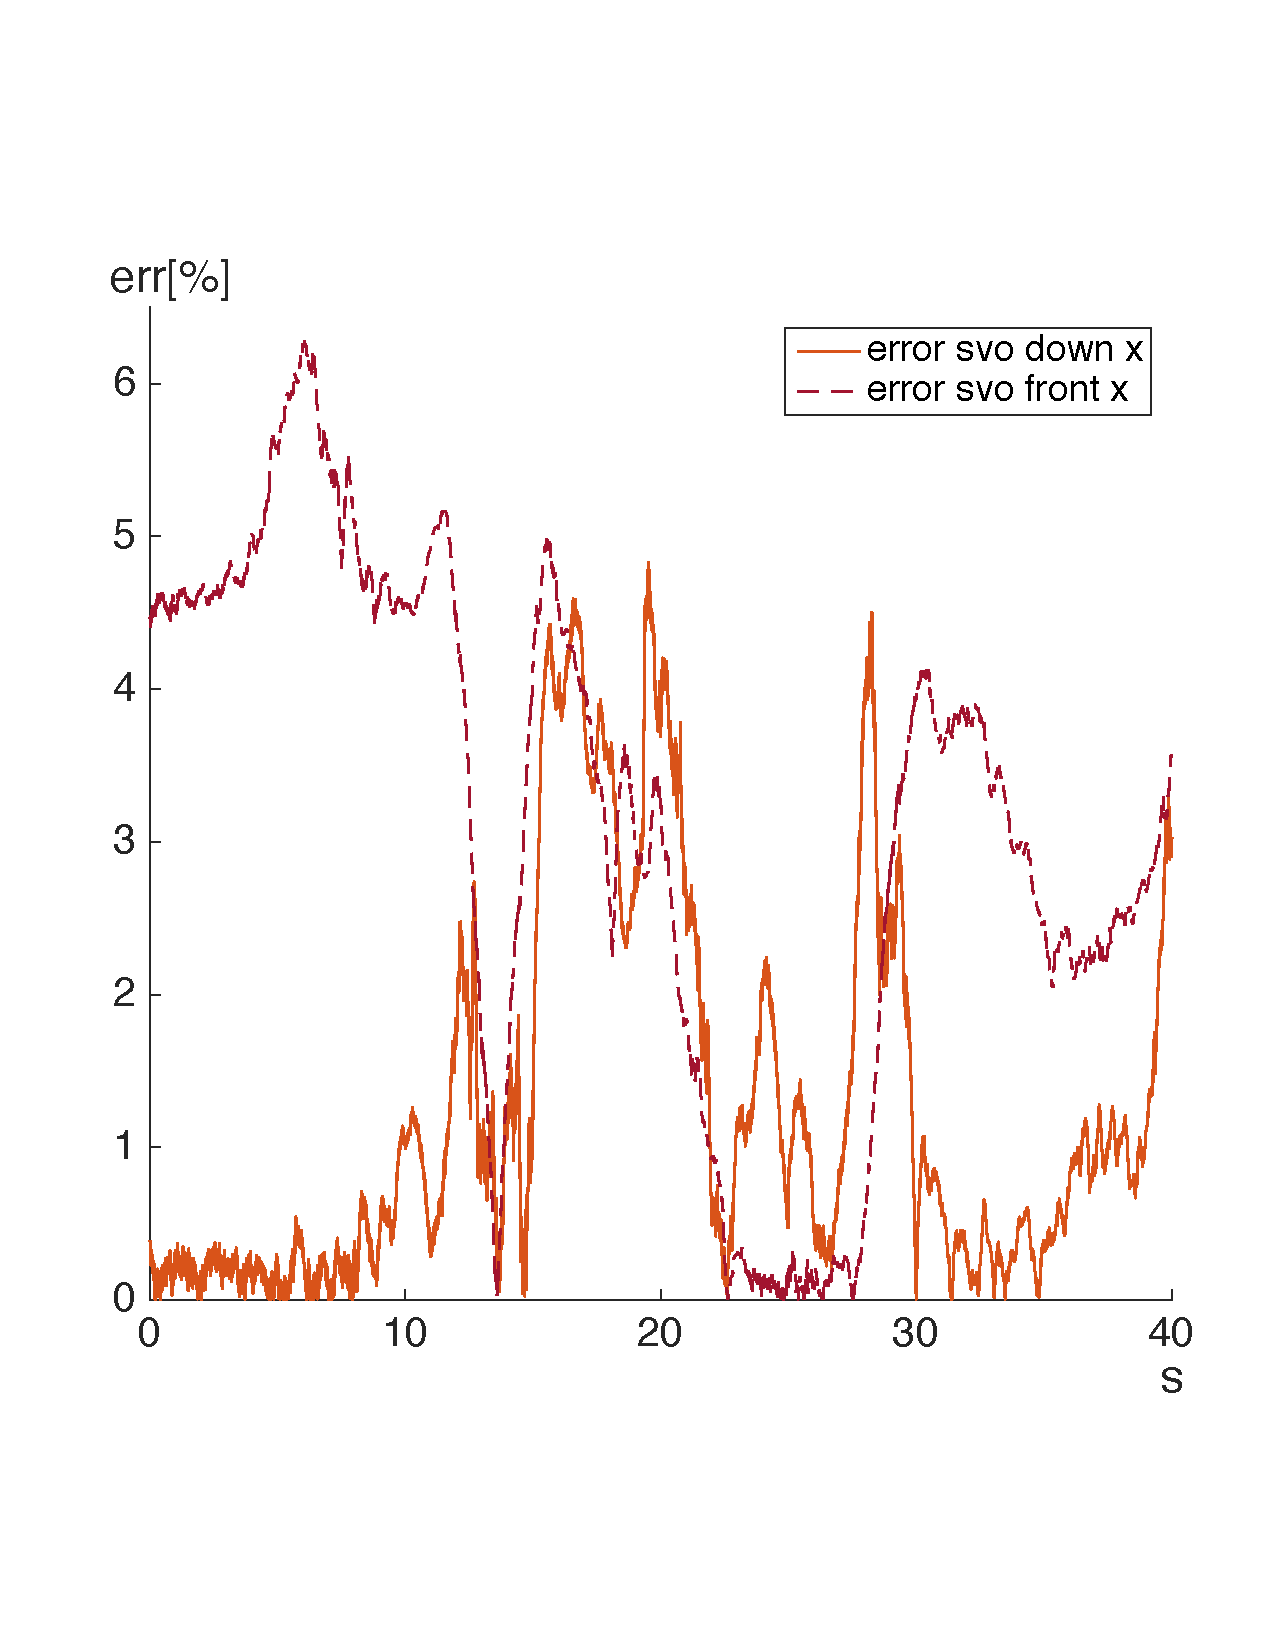
\includegraphics[width=\textwidth]{img/err_perc_2_svo_x.pdf}
%        \label{fig:perc_errorone}
%   \end{subfigure} \hfill
%   \begin{subfigure}[b]{0.3\textwidth}
%        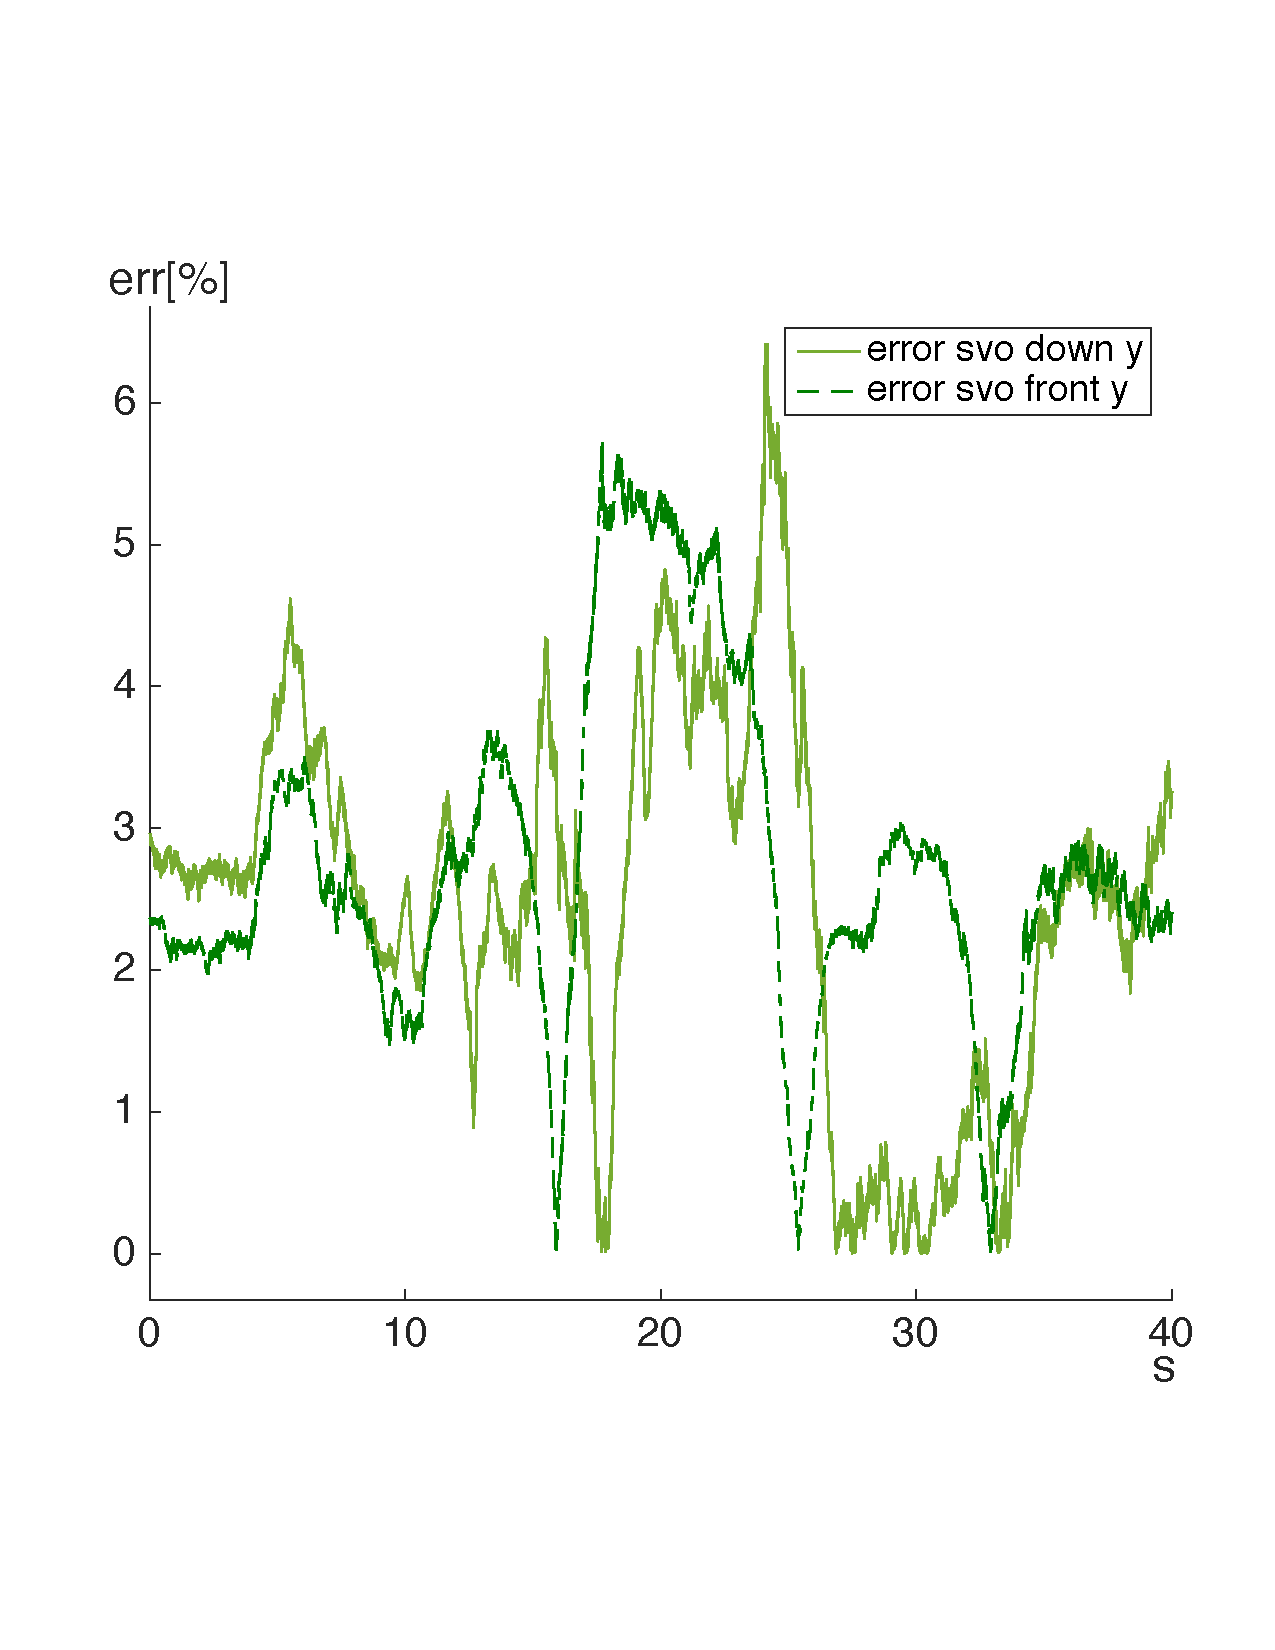
\includegraphics[width=\textwidth]{img/err_perc_2_svo_y.pdf}
%        \label{fig:perc_errortwo}
%   \end{subfigure}\hfill
%   \begin{subfigure}[b]{0.3\textwidth}
%        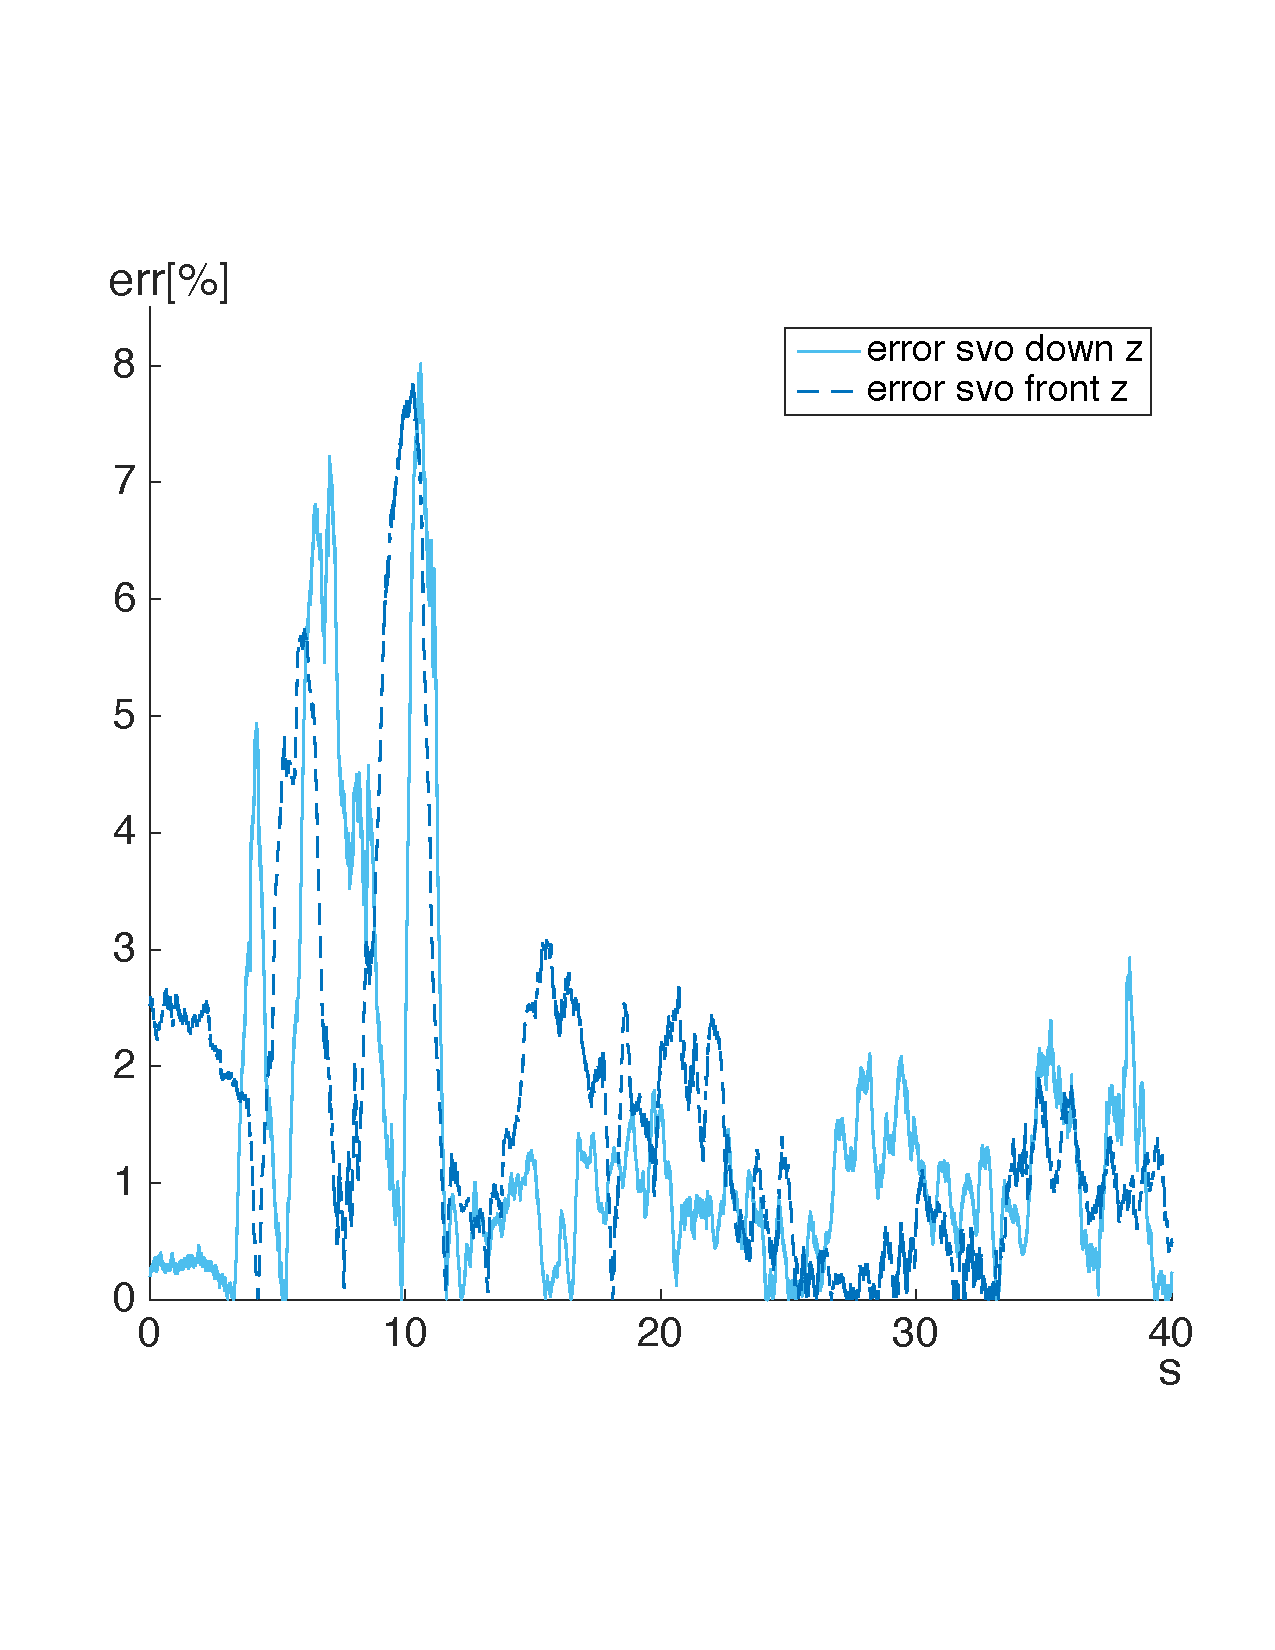
\includegraphics[width=\textwidth]{img/err_perc_2_svo_z.pdf}
%        \label{fig:perc_errorthree}
%   \end{subfigure}
%  \caption{Percentage error, in each dimension, between the two version of SVO and the ground truth given by the OptiTrack. The quad traveled more or less 2m in x,y direction and 1m in z.}
%  \label{fig:perc_error}
%\end{figure} 

From Fig.~\ref{fig:comparision_svo_trajectory} we can see that the main problem is the scale factor. The scale factor is estimated at the beginning, tracking features of the images and setting their depth at a known value. If there is an error in this initialization then all the world is scaled and will result bigger or smaller than the reality.


%
%\subsection{Drifting}
%We made other experiments to understand if the current version of frontlooking-fisheye-SVO is good enough to fly with it.\\ 
%We performed several manual flights in the flyingroom, with the same results: generally SVO is estimating a correct and precise state of the quad, but sometimes it occurs that the state estimation drifts.\\
%For example, the dataset shown in Fig.~\ref{fig:svo_position_driftind} is related to a flight in which three times the SVO estimation drifted with respect to the real world in all three axes. We highlighted in the figure these moments.\\
%
%\begin{figure}[!htbp]
%  \centering
%  \begin{subfigure}[b]{0.35\textwidth}
%        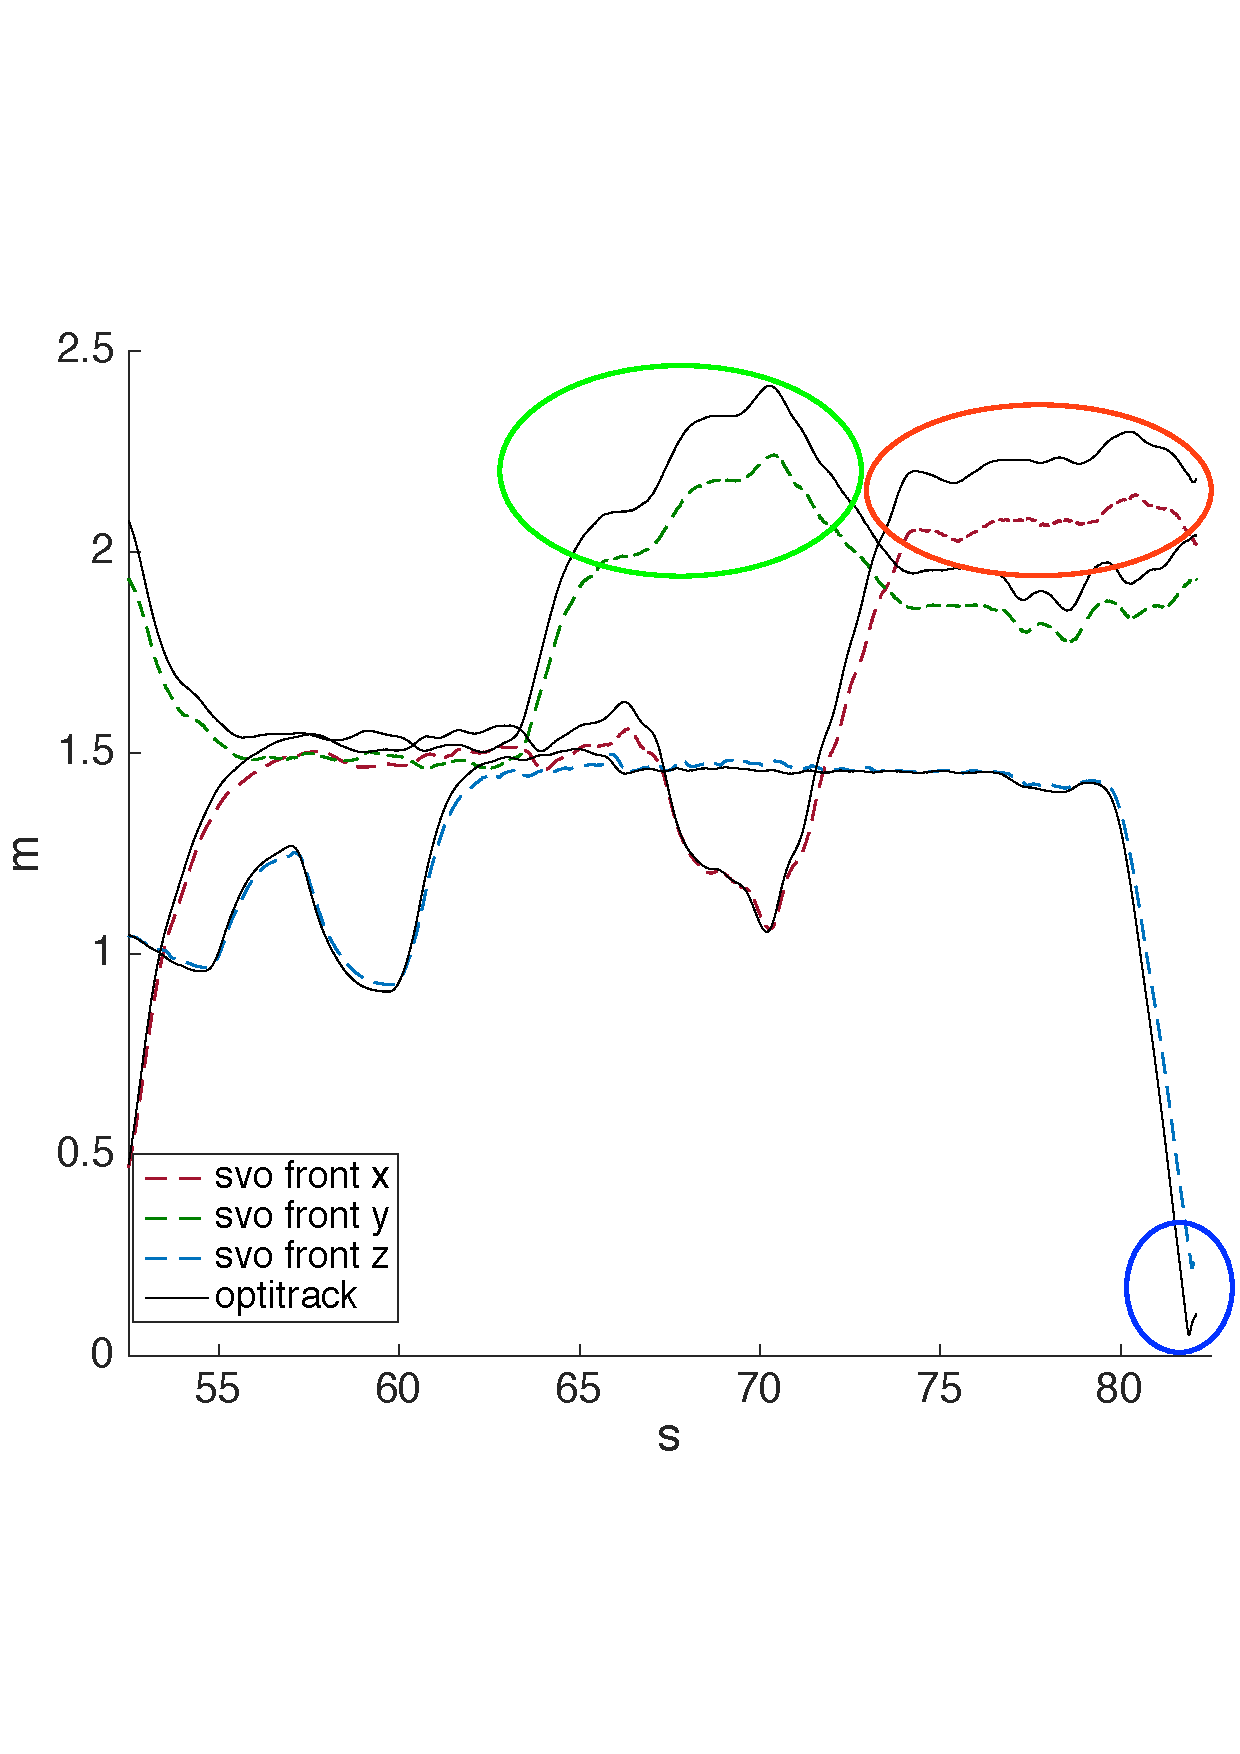
\includegraphics[width=\textwidth]{img/fly_with_landing_position.pdf}
%        \label{fig:comparision_svo_position_drifting}
%   \end{subfigure} \hfill
%   \begin{subfigure}[b]{0.3\textwidth}
%        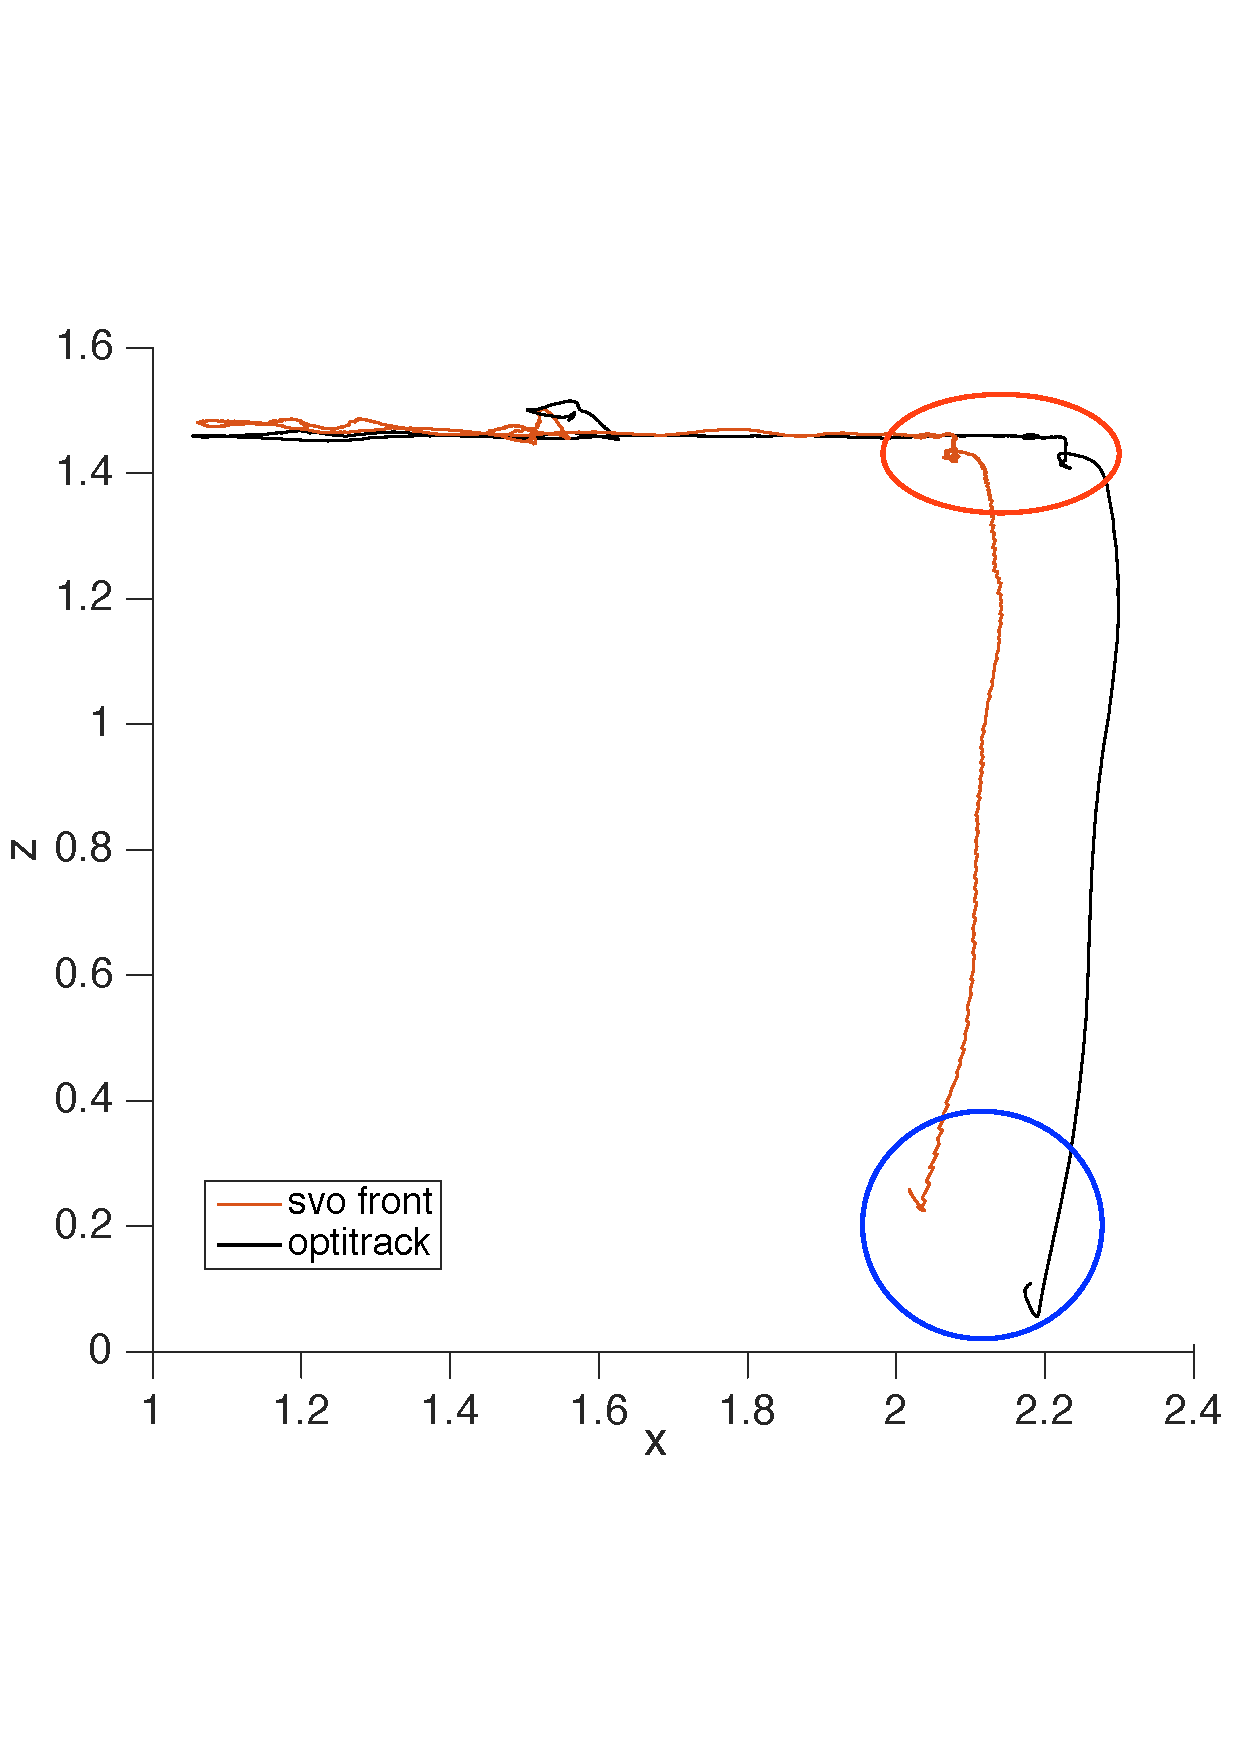
\includegraphics[width=\textwidth]{img/fly_with_landing_trajectory_x.pdf}
%        \label{fig:comparision_svo_position_drifting_x}
%   \end{subfigure}\hfill
%   \begin{subfigure}[b]{0.3\textwidth}
%        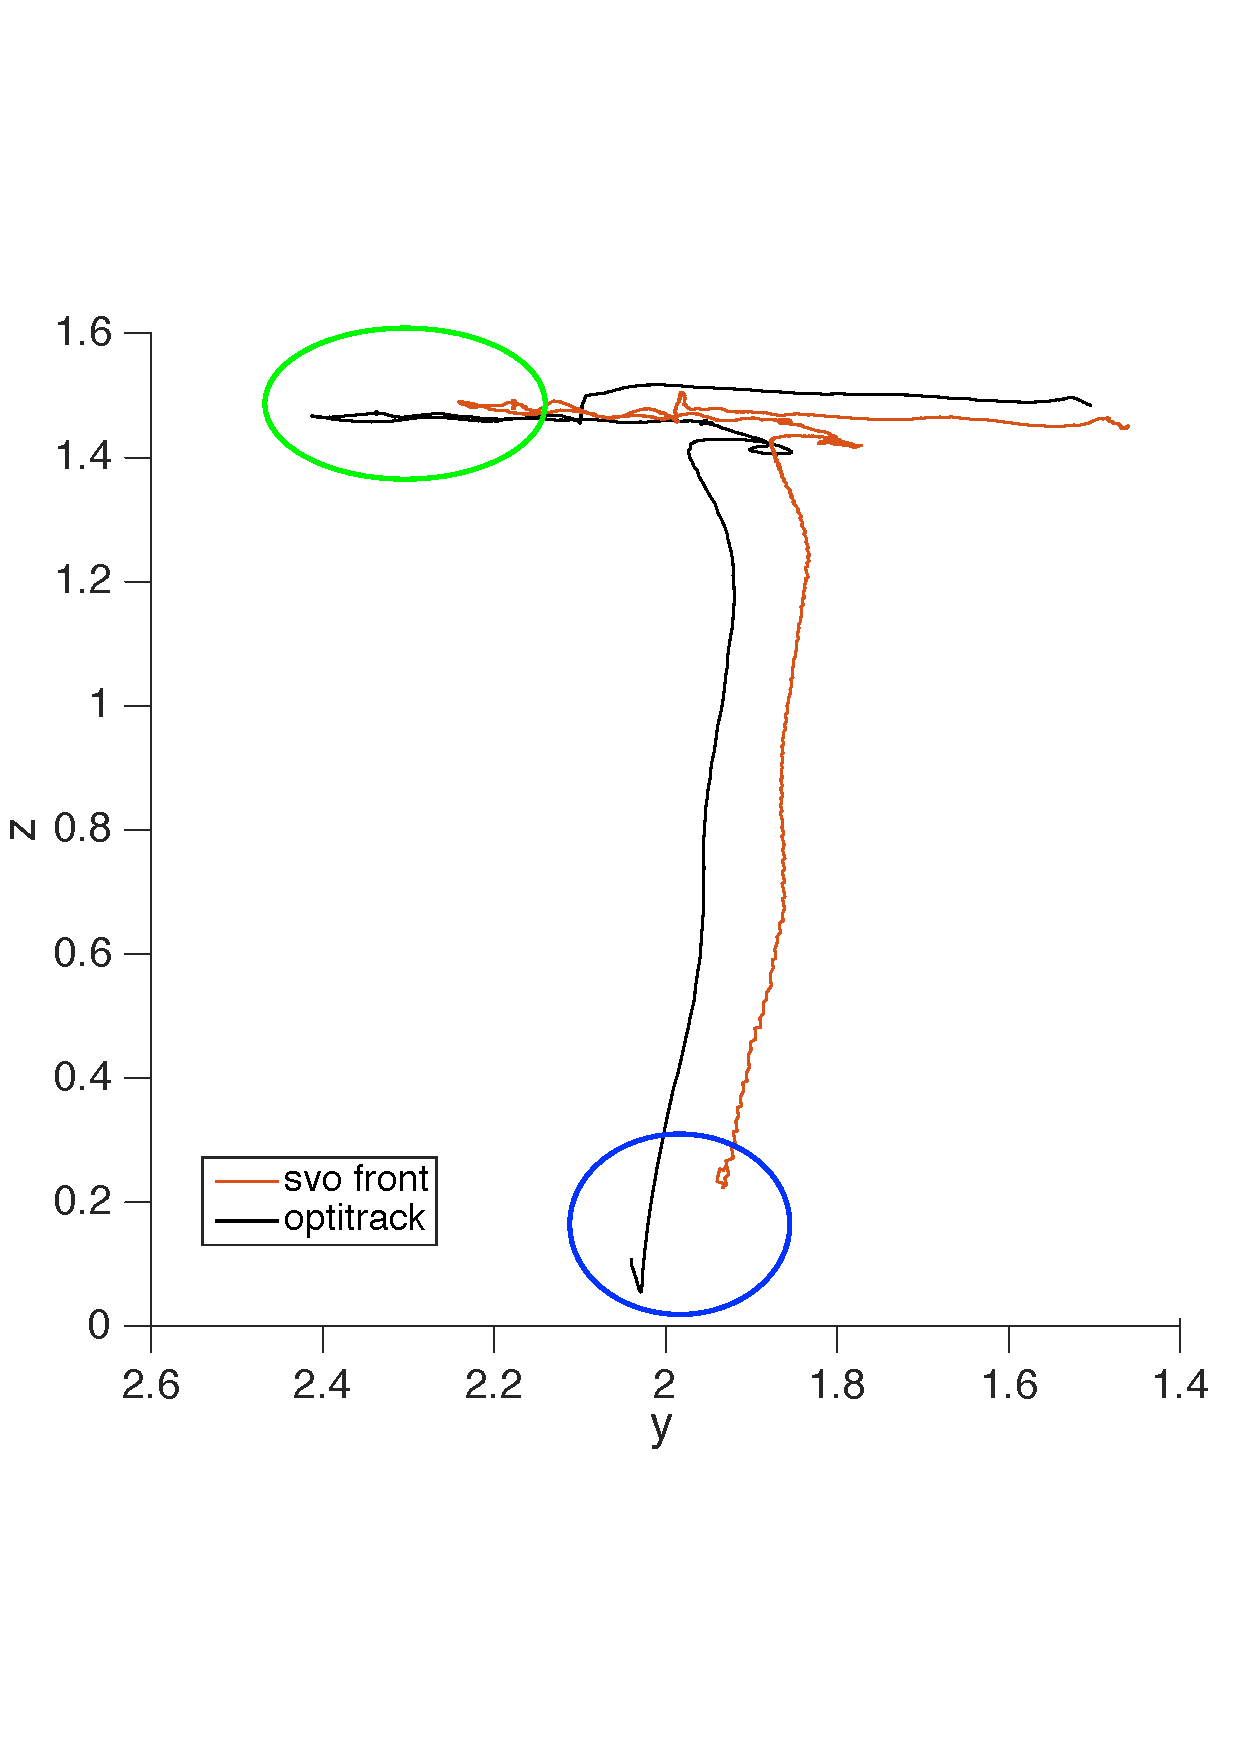
\includegraphics[width=\textwidth]{img/fly_with_landing_trajectory_y.pdf}
%        \label{fig:comparision_svo_position_drifting_y}
%   \end{subfigure}
%  \caption{Manual flight in which SVO drifted away from the reality. Highlighted by circles are the moment in which these drifts happened and there are the correspondences between the time domain and the trajectory. }
%  \label{fig:svo_position_driftind}
%\end{figure} 
%
%The reasons for this behavior can be related to the lack of features that the vertical walls in the flyingroom has. As a matter of fact if there are no enough distinctive features the visual odometry can drift. TODO ???

%\subsection{Fast flight}
%In the final challenge the moving car will move at \SI{15}{\km \per \hour} that means \SI{4.17}{\meter \per \second}. In order the quadrotor to be able to follow and land on the platform it must flight faster then this velocity.\\
%With the quadrotor used in this experiments we can reach velocity up to \SI{2}{\meter \per \second}.
%We made some experiments to understand if the state estimation with the front looking camera it is precise at this speed.\\
%The results are reported in Figure \ref{fig:highspeed} that shows a behavior similar


\section{Base detection and tracking}
Several experiments were performed both in simulation and in the real world to evaluate the performance of the platform state estimation.

\subsection{From high altitude}
We do not require the state estimation from high altitude to be very precise, since we need a rough estimation of the position of the platform.
The precision of the estimation depends on the altitude from which the quadrotor is tracking the base and, with the designed EKF, we obtain a reliable estimate of the base state.\\
Figures~\ref{fig:ekf_real_world_high} and \ref{fig:ekf_high_altitude_comparison} show the result of different experiments both in the real world and simulation.\\

In real world experiments we tested the detector with the platform described before. To have a comparison with a ground truth we did the experiments in the RPG flyingroom, where the position of the platform from the OptiTrack is available. In these experiments the quadrotor cannot reach high altitude and it tracks the moving platform from \SI{2}{\meter}.
\begin{figure}[!htbp]
  \centering
   \begin{subfigure}[b]{0.45\textwidth}
        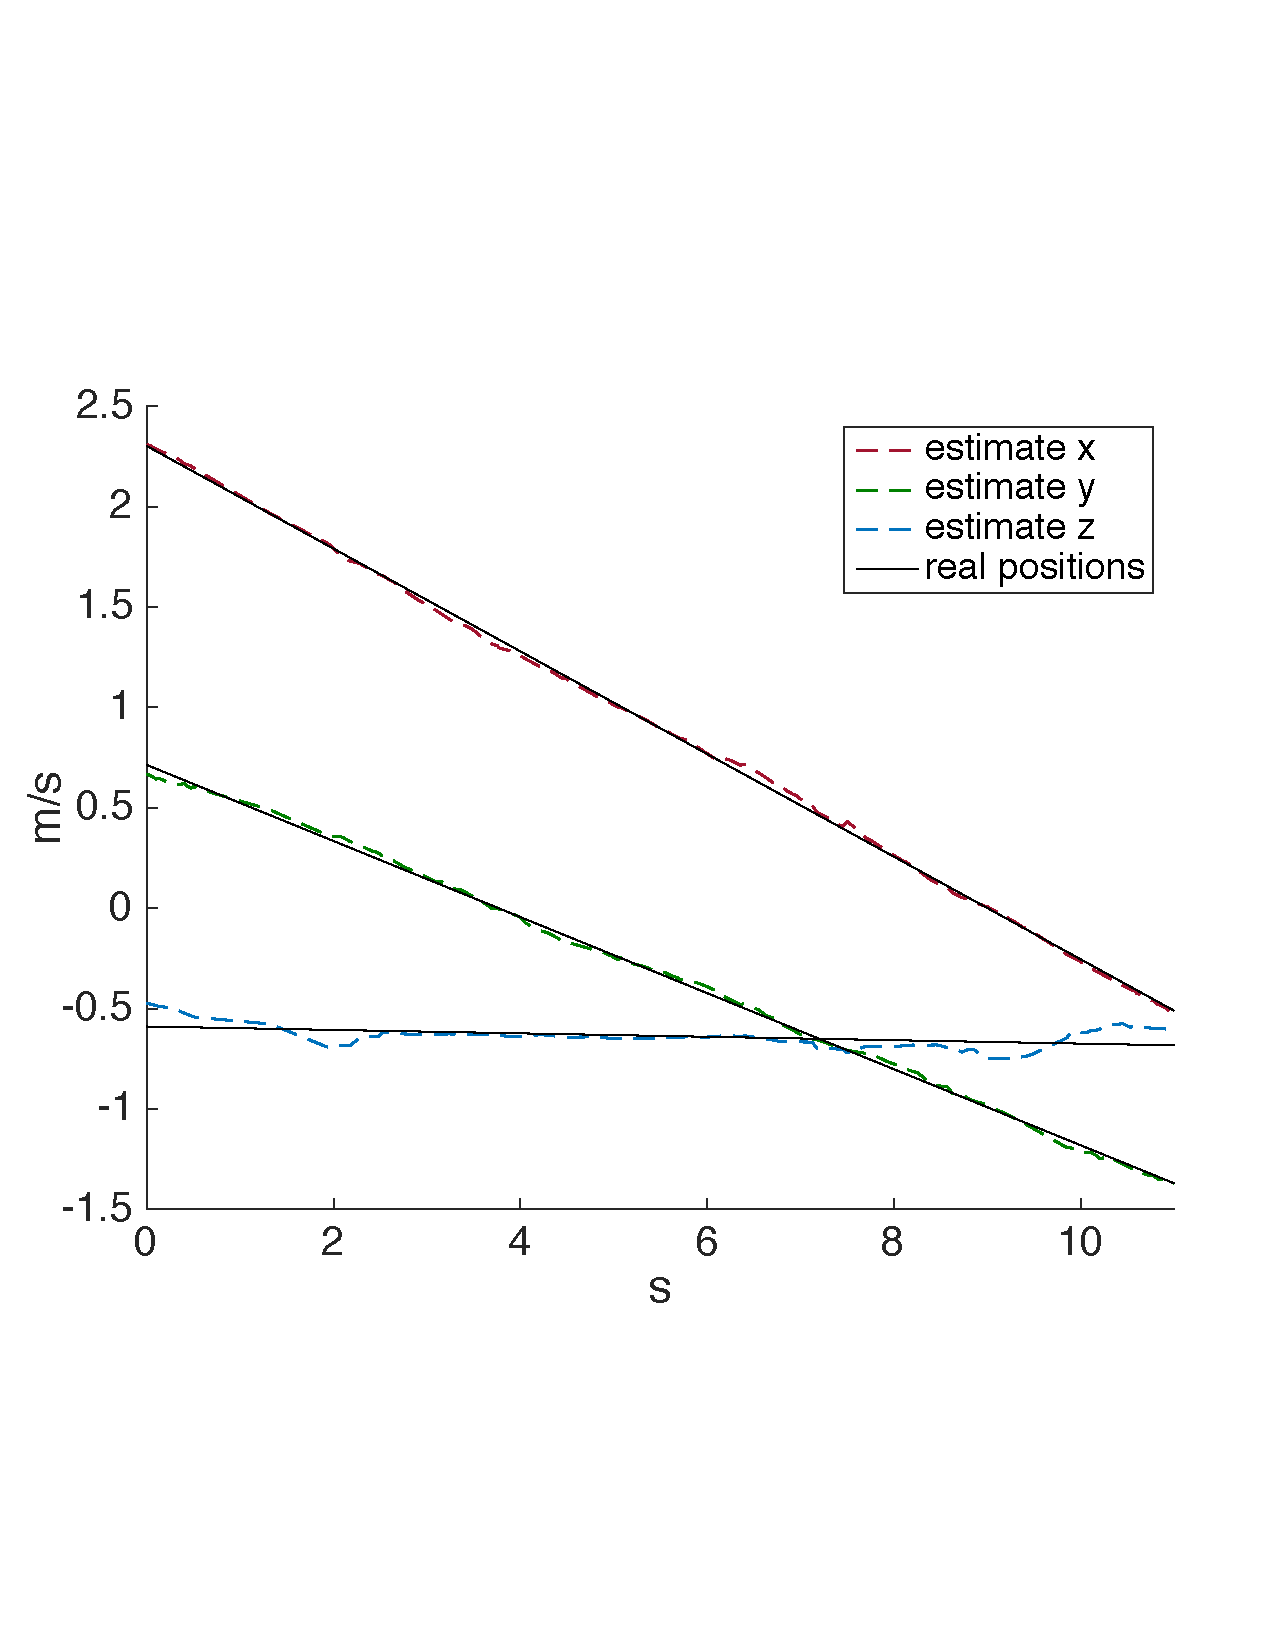
\includegraphics[width=\textwidth]{img/tag_moving_real_world_pos_high_altitude.pdf}
        \caption{Position }
        \label{fig:one_ekf_real_world_high}
   \end{subfigure}\hfill
   \begin{subfigure}[b]{0.45\textwidth}
        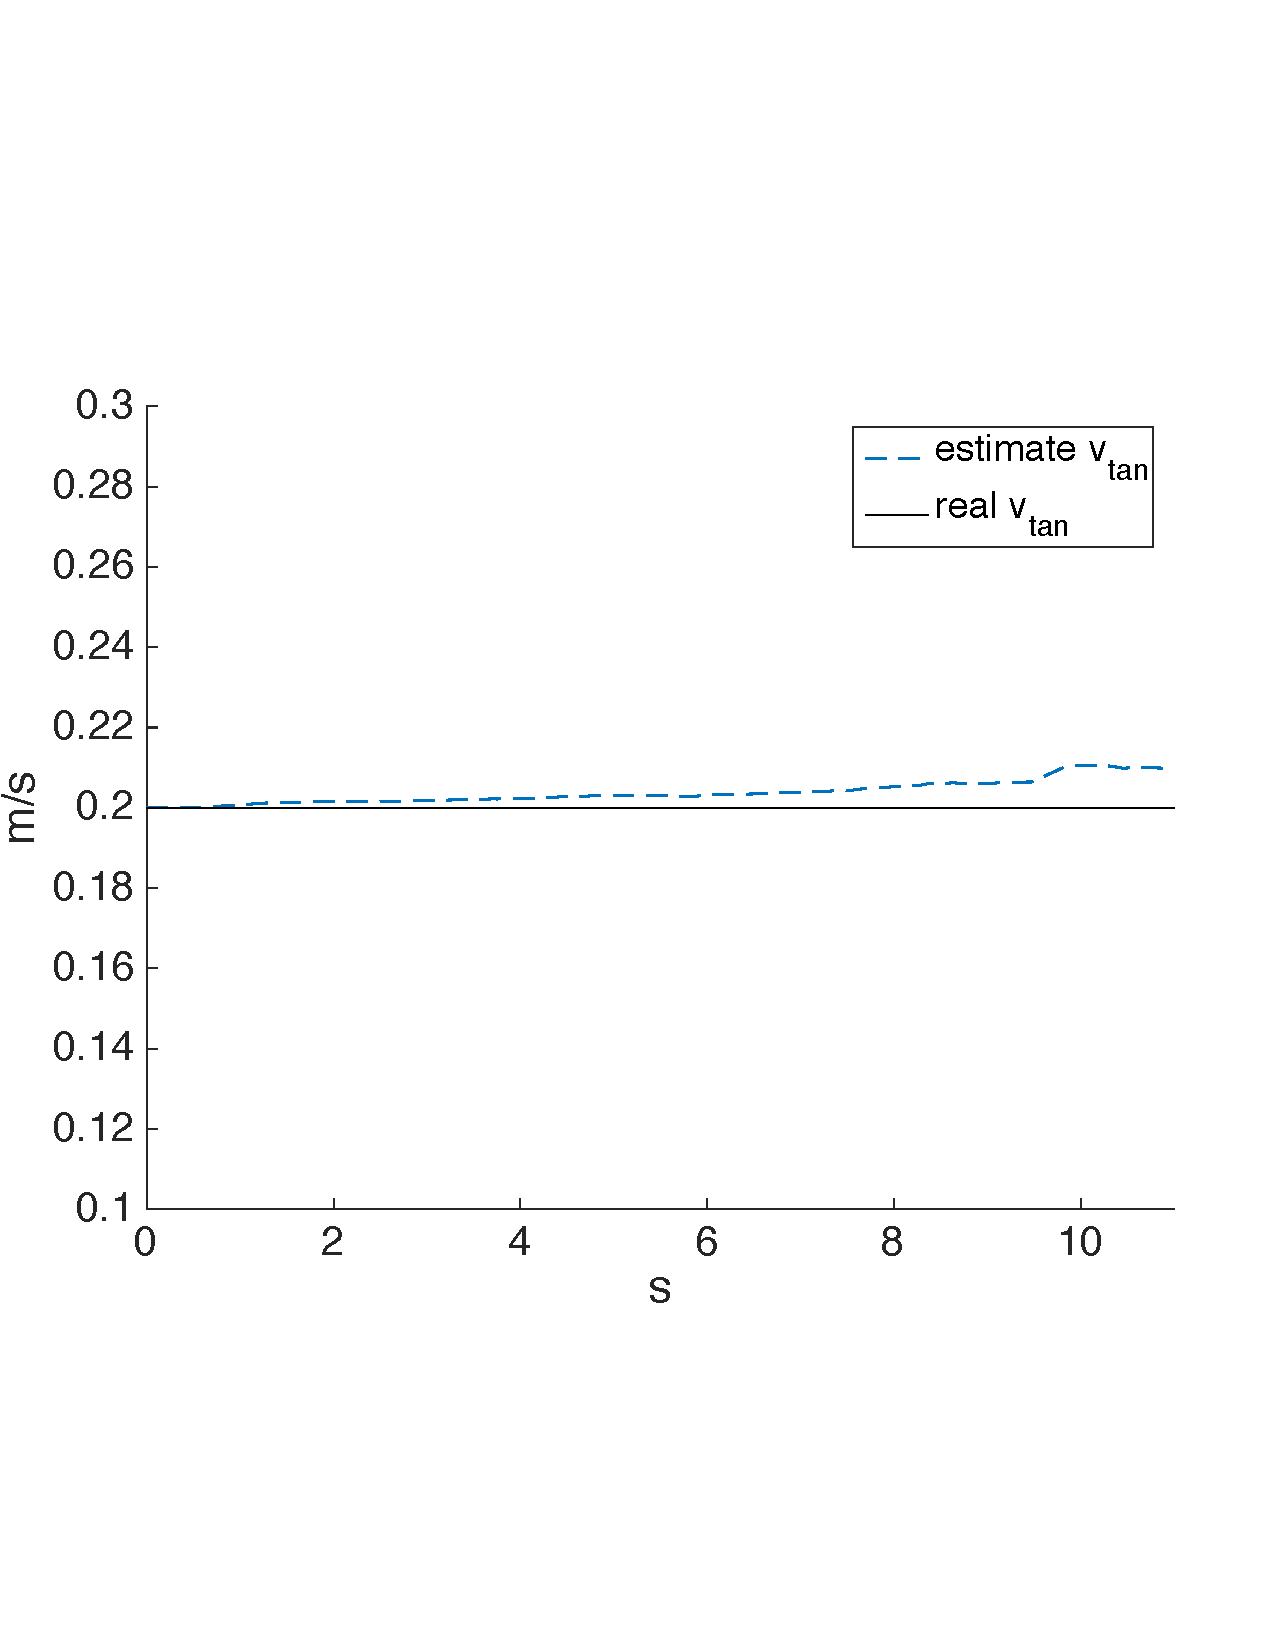
\includegraphics[width=\textwidth]{img/tag_moving_real_world_vel_high_altitude.pdf}
        \caption{Velocity}
        \label{fig:two_ekf_real_world_high}
   \end{subfigure}
  \caption{Real world experiment. Comparison between estimate position and velocity with the ground truth values for a  platform moving at \SI{0.2}{\meter \per \second}. The estimate position  is taken from \SI{2}{\meter} height and has a RMSE of \SI{5}{\centi \meter} in $x,y$ and \SI{10}{\centi \meter} in $z$.}
  \label{fig:ekf_real_world_high}
\end{figure} 

In simulation we can track the platform from really high altitude. Figure~\ref{fig:ekf_high_altitude_comparison} shows the result of a tracking from \SI{15}{\meter} height. Of course, in this case the estimate is no long very precise, because the precision of the pose estimation of the platform decreases at high altitude. 

\begin{figure}[!htbp]
  \centering
  \begin{subfigure}[b]{0.5\textwidth}
        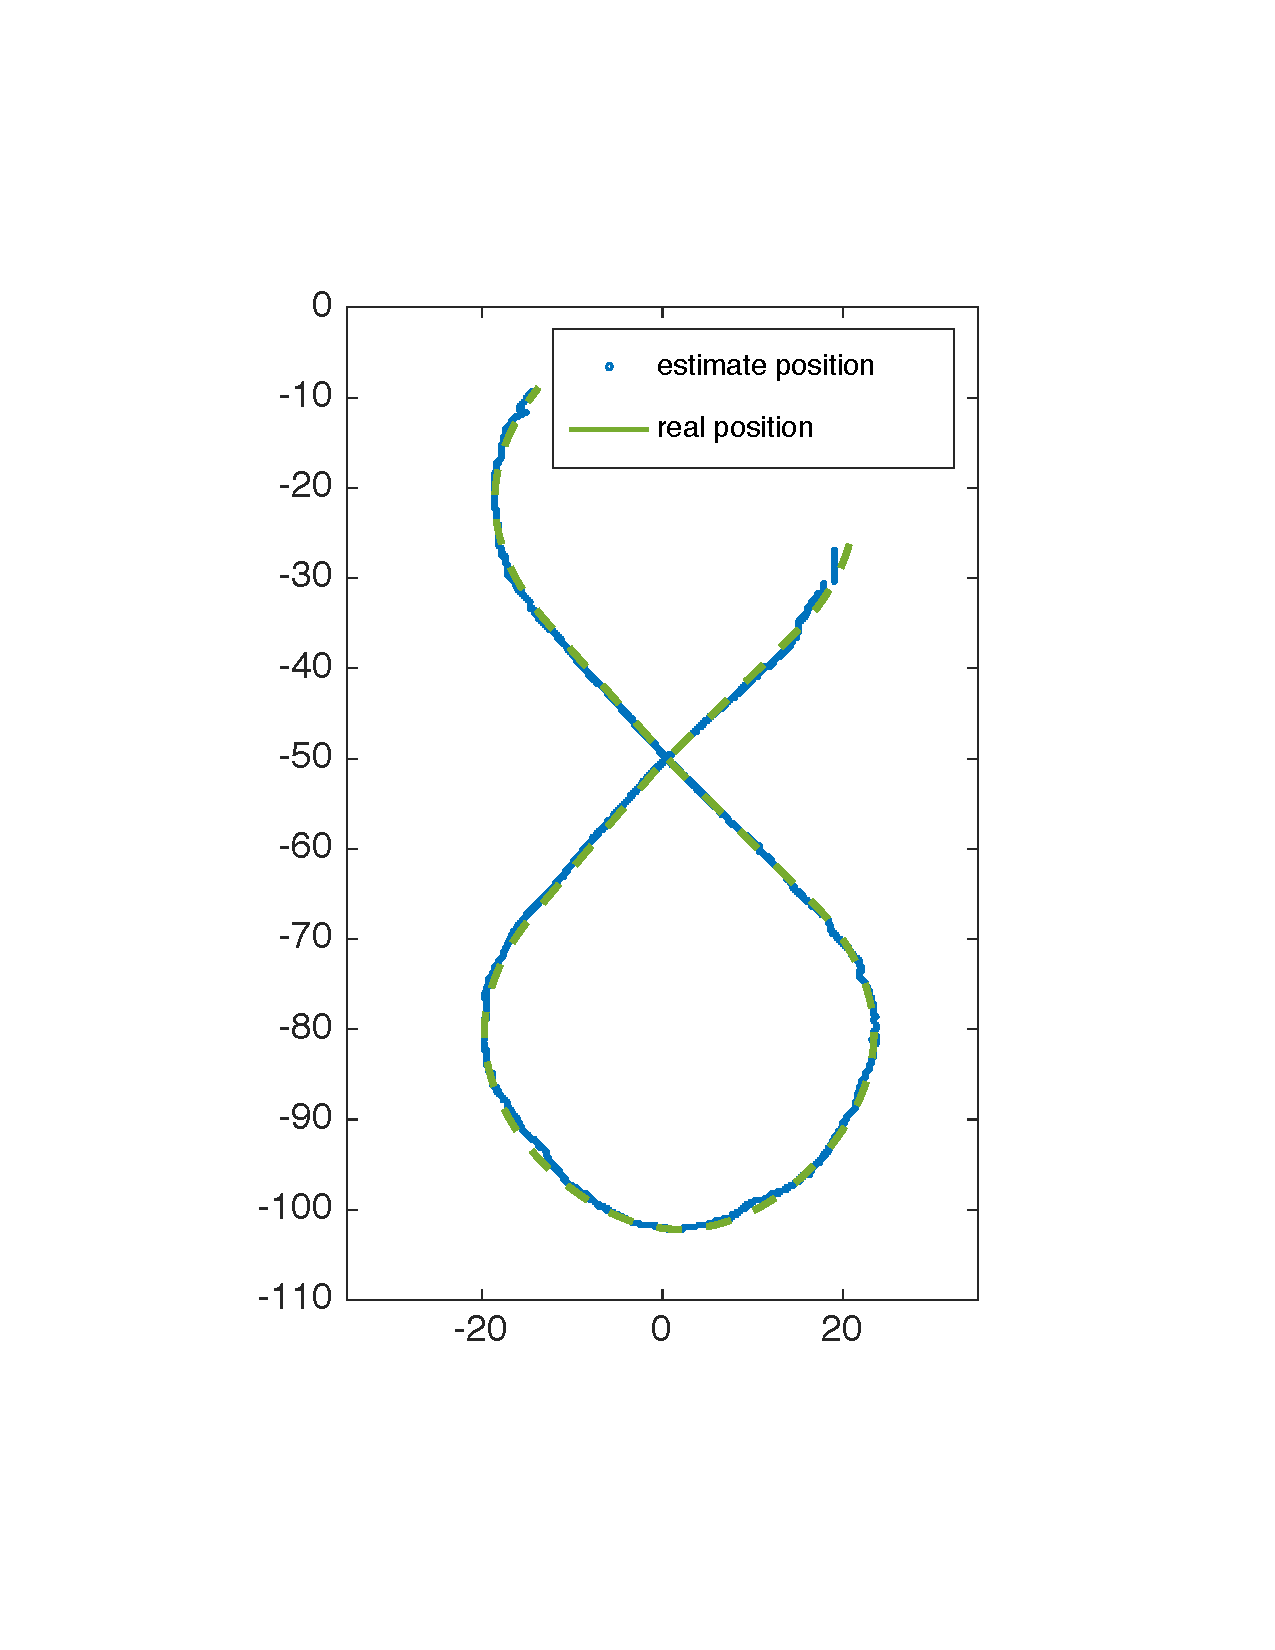
\includegraphics[width=\textwidth]{img/high_altitude_error_xy.pdf}
        \caption{Trajectory}
        \label{fig:one}
   \end{subfigure} \\
   \begin{subfigure}[b]{0.35\textwidth}
        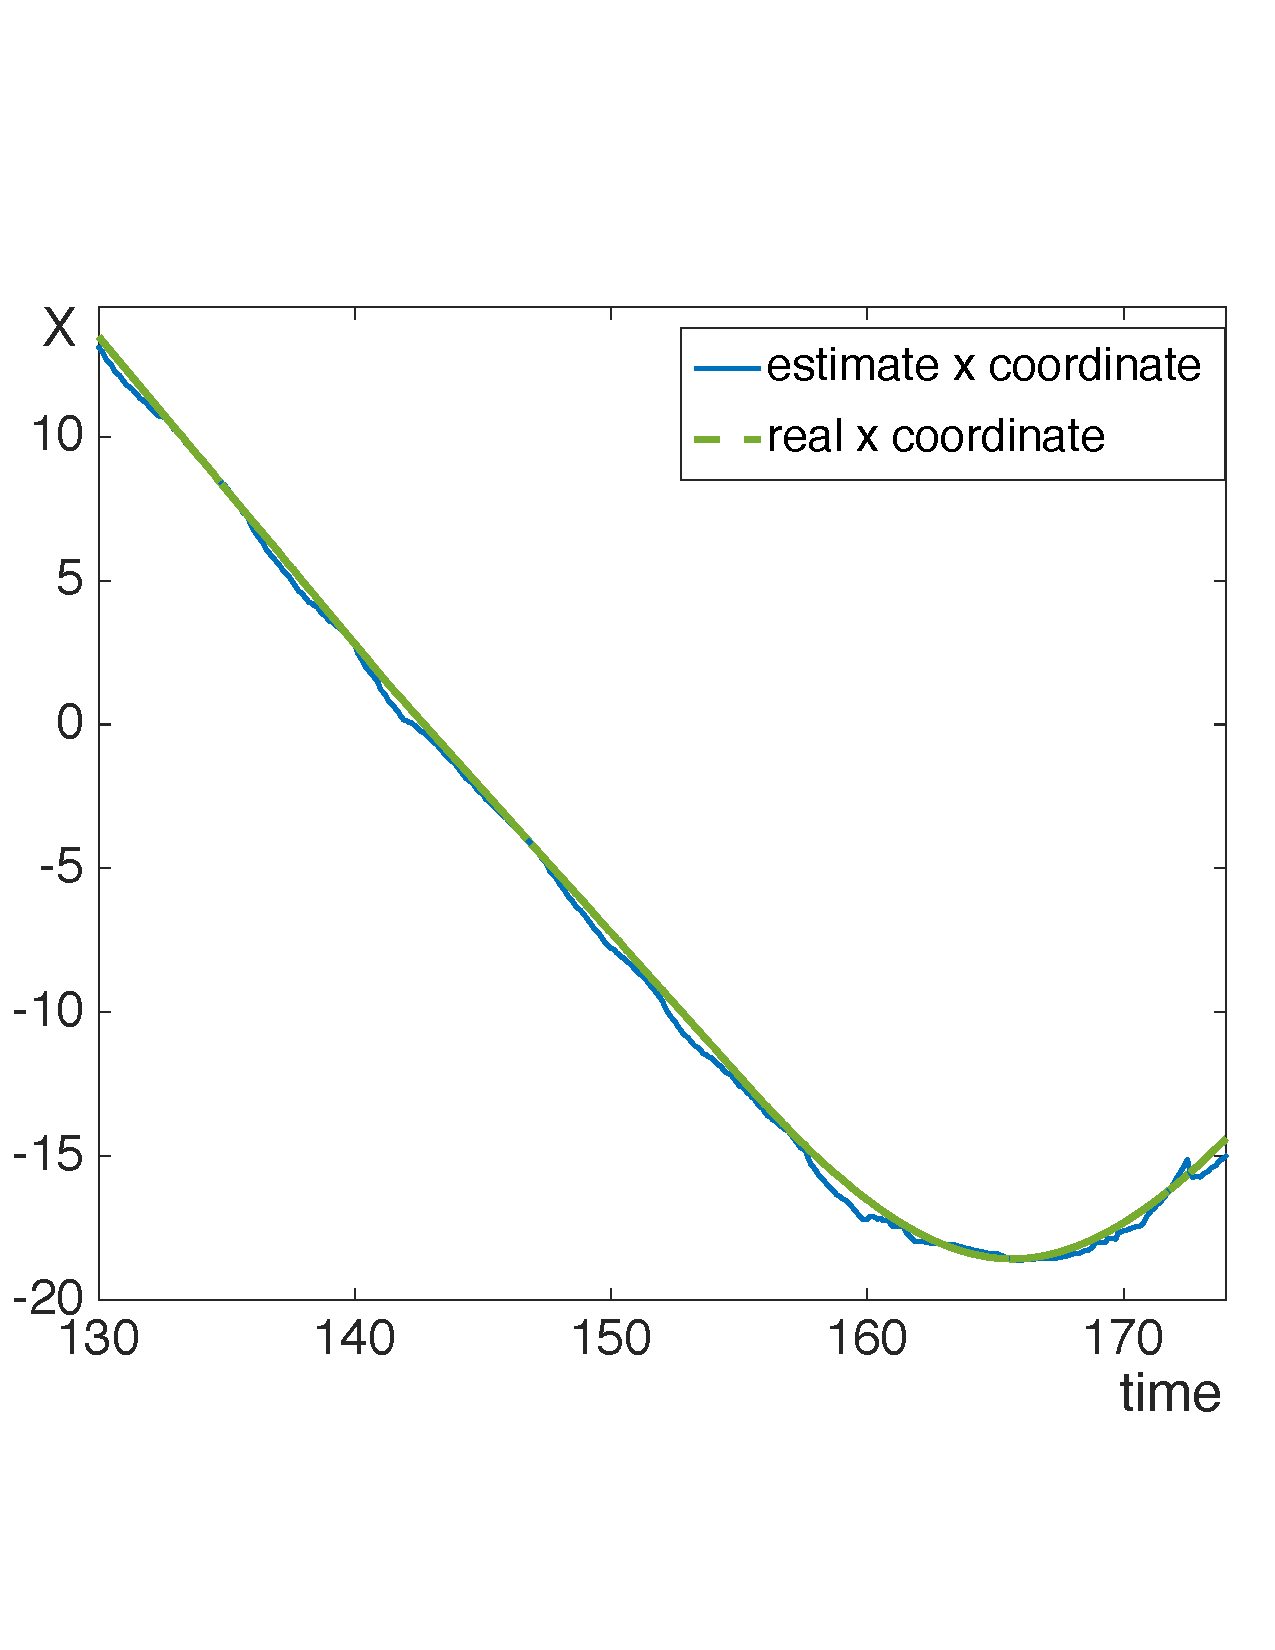
\includegraphics[width=\textwidth]{img/high_altitude_error_x.pdf}
        \caption{x }
        \label{fig:one}
   \end{subfigure}
   \begin{subfigure}[b]{0.35\textwidth}
        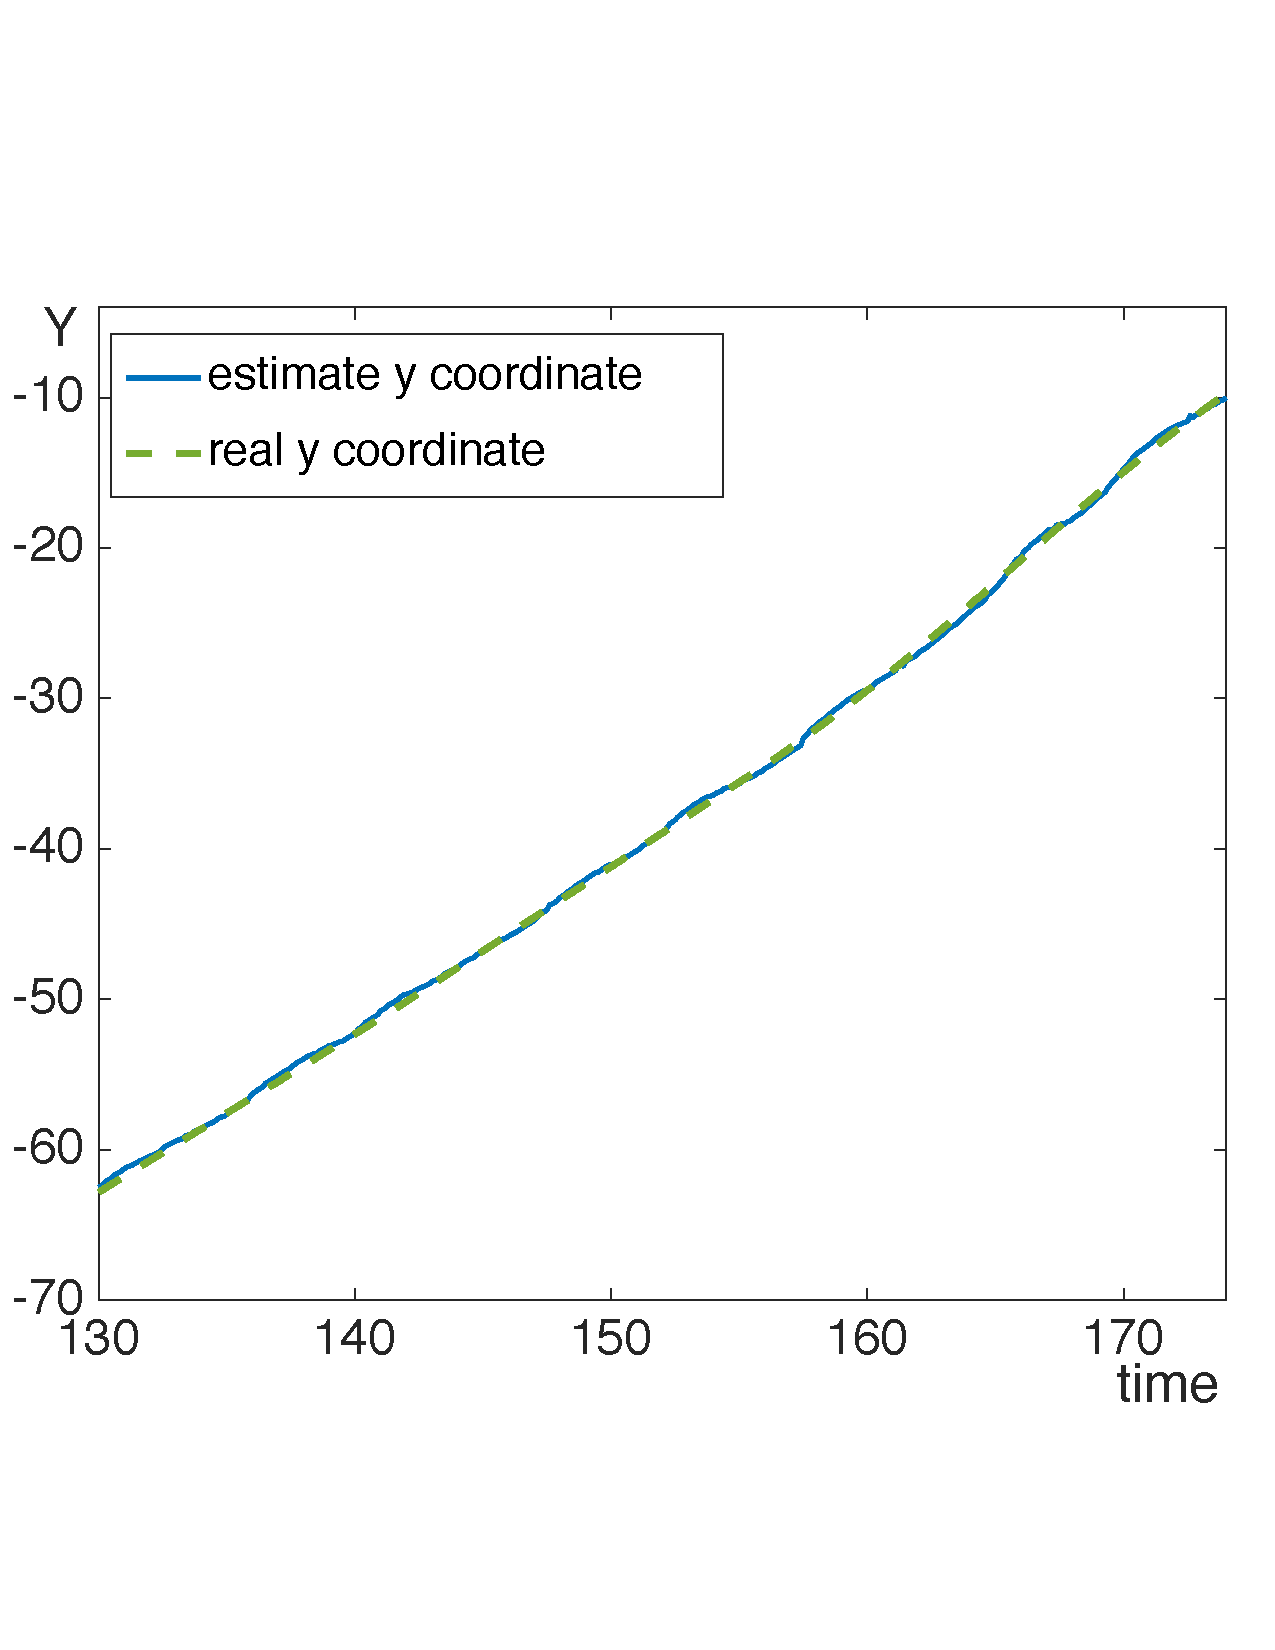
\includegraphics[width=\textwidth]{img/high_altitude_error_y.pdf}
        \caption{y}
        \label{fig:two}
   \end{subfigure}
  \caption{Comparison between estimate position (blue dots) and real position (green line) in simulation. The platform is moving in the 8 shape path at \SI{1.5}{\meter \per \second} and the quadrotor explores the area at \SI{15}{\meter} of altitude.}
  \label{fig:ekf_high_altitude_comparison}
\end{figure} 

As one can see from Fig.~\ref{fig:ekf_high_altitude_error}, the estimation error can be really high during this phase, as shown by the average error in $x$ and $y$ directions and the correspondent RMSE from a searching at \SI{15}{\meter} of altitude. In general, the state estimate has a RMSE of \SI{0.4}{\meter}.\\
Even if they are not very accurate, this data are good enough to perform the first stages of the state machine.
\begin{figure}[!ht]
    \centering
    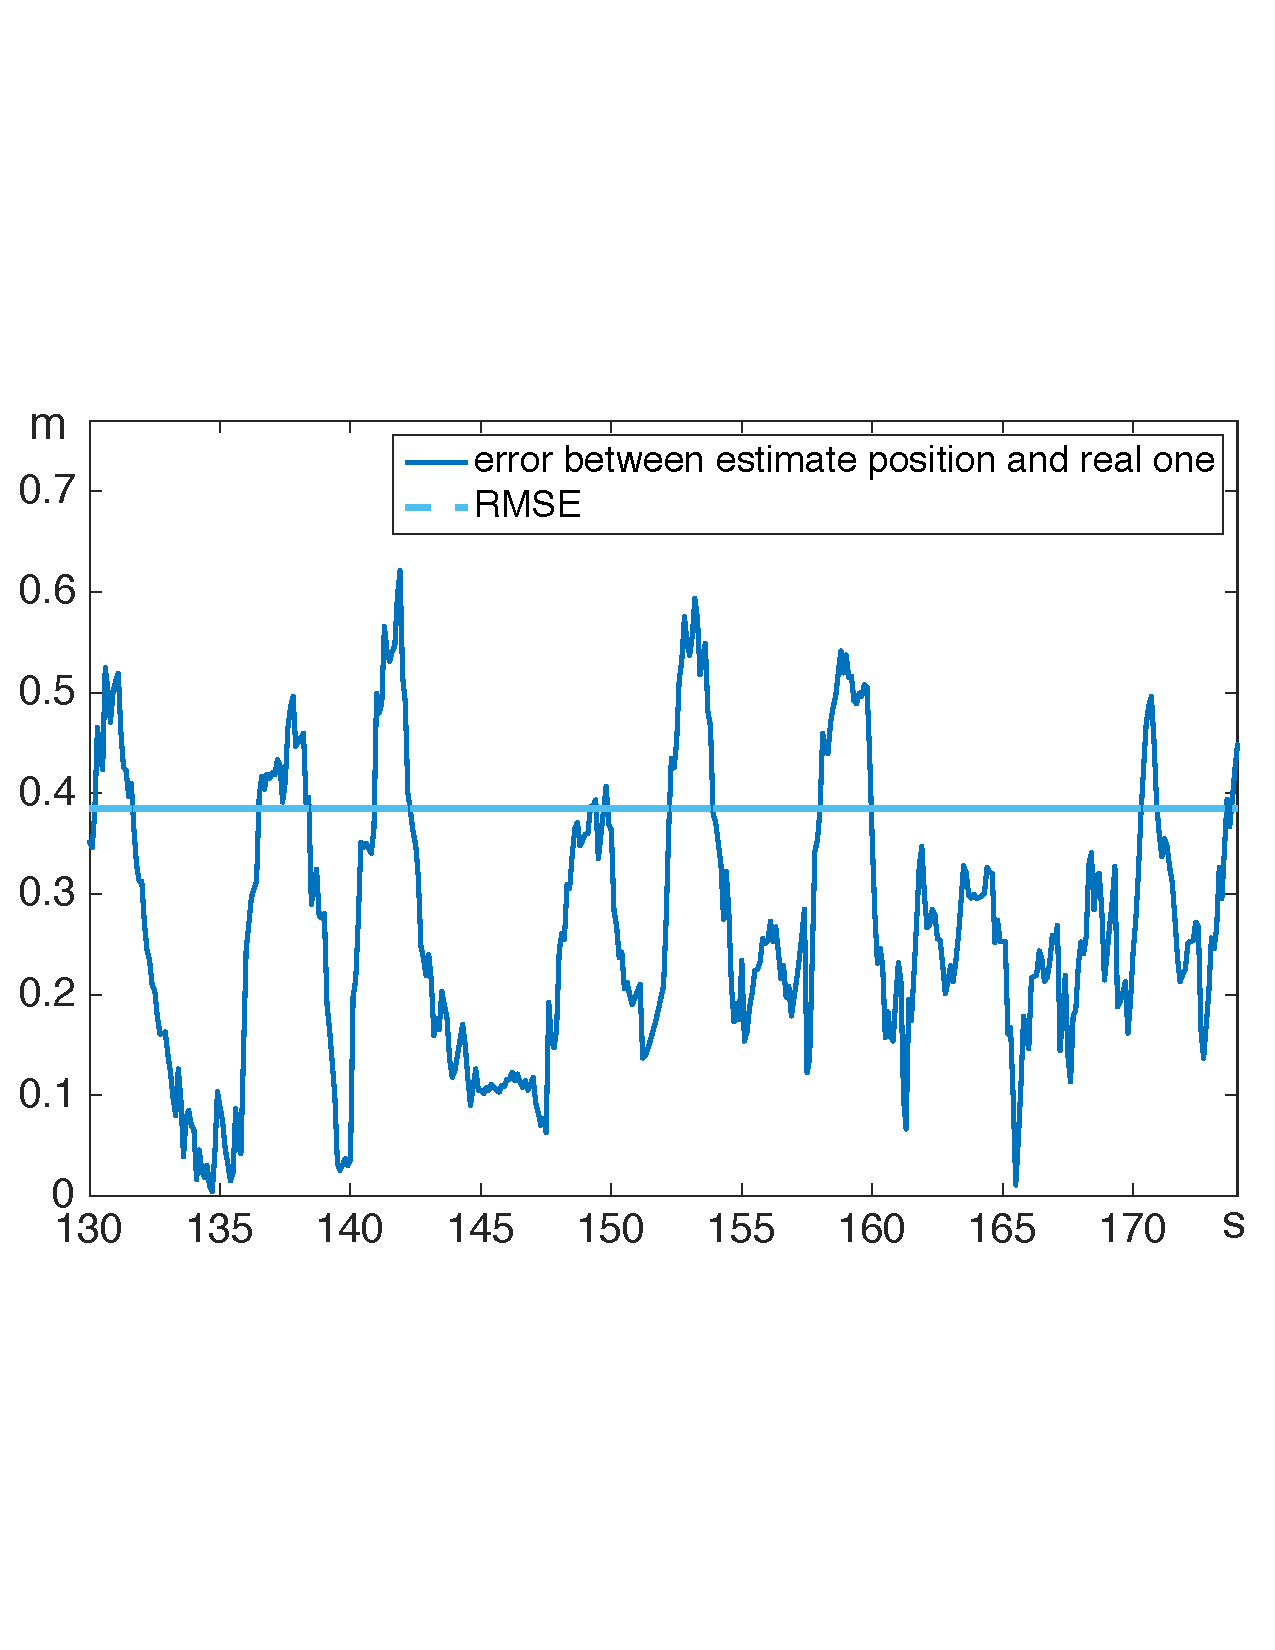
\includegraphics[width=0.6\textwidth]{img/high_altitude_error.pdf}
      \caption{Average error between estimate and real x,y coordinate. The RMSE is below \SI{0.4}{\meter}. This precision is sufficient to estimate the type of movement of the base.}
    \label{fig:ekf_high_altitude_error}
\end{figure}


\subsection{From low altitude}
\subsubsection{Different AR-Tag detector}
In the real world implementation we tried several different tag detector ROS packages, such as RPG-April-Tags \cite{rpgapriltags} that uses the AprilTags library \cite{apriltagslibrary}, AR-Sys \cite{arsys} and AR-Track-Alvar \cite{artrackalvar}.\\
All of them have some strengths and weaknesses and we compared the most important features to understand which detector is the more suitable for our purpose:
\begin{itemize}
\item \textbf{Light conditions}: all these methods use the edge based approach, so the results is similar in different light conditions.
\item \textbf{Final pose}: all trackers solve a PnP Problem to find the 6DoF pose of the camera that minimizes the reprojection error of the points in the image. The final result is the transformation between the tag and the camera. RPG-AprilTag has also the possibility to return a 4DoF pose (perfect for our application), saving some computation.
\item \textbf{Multiple tags}: AR-Sys and AR-Track-Alvar have the ability to directly track multiple tags or single target composed by multiple tags.
\item \textbf{Precision}: we measure the error at \SI{1}{\meter} distance from the tag
\begin{itemize}
\item RPG-April-Tags: $\pm$ 1 pixel 
\item AR-Sys: $\pm$ 2 pixel 
\item AR-Track-Alvar: $\pm$ 1 pixel 
\end{itemize}
\item \textbf{Frequency}: on the quadrotor the performance of the three tracker where quite different
\begin{itemize}
\item RPG-April-Tags: $~$\SI{1}{\Hz}
\item AR-Sys: $~$\SI{4}{\Hz}
\item AR-Track-Alvar: $~$\SI{1}{\Hz}
\end{itemize}
\end{itemize}

\paragraph{AR-Sys}
In our final implementation we decided to use AR-Sys because of its computational efficiency. AR-Sys is 3D pose estimation ROS package that uses ARUco marker boards \cite{Aruco2014}.\\
This package guarantees a good error correction in the identification of a specific tag, and, more interesting for our application, a solution to the occlusion problem using multiple markers: it can track the pose of boards composed by multiple tags, considered as a single unit. We can define one of these boards in an XML file. In this file all the tags, that compose the board, are listed. The tags are defined with an ID and with a relative position with respect to a master tag (the first in the list) that defines the center of the cumulative target.
The pose of the camera is given with respect to this master tag. This feature guarantees more stable pose estimates and robustness to the occlusion of a part of the platform.

Very accurate pose estimation is obtain when the AR tags are used. Generally, the error in the $x,y$ coordinate is less then \SI{7}{\centi \meter}, in the $z$ direction is about \SI{3}{\centi \meter}.\\
The following figures show different experiments in the real world and in the simulation with different velocities and initial values.\\

\begin{figure}[!htbp]
  \centering
   \begin{subfigure}[b]{0.45\textwidth}
        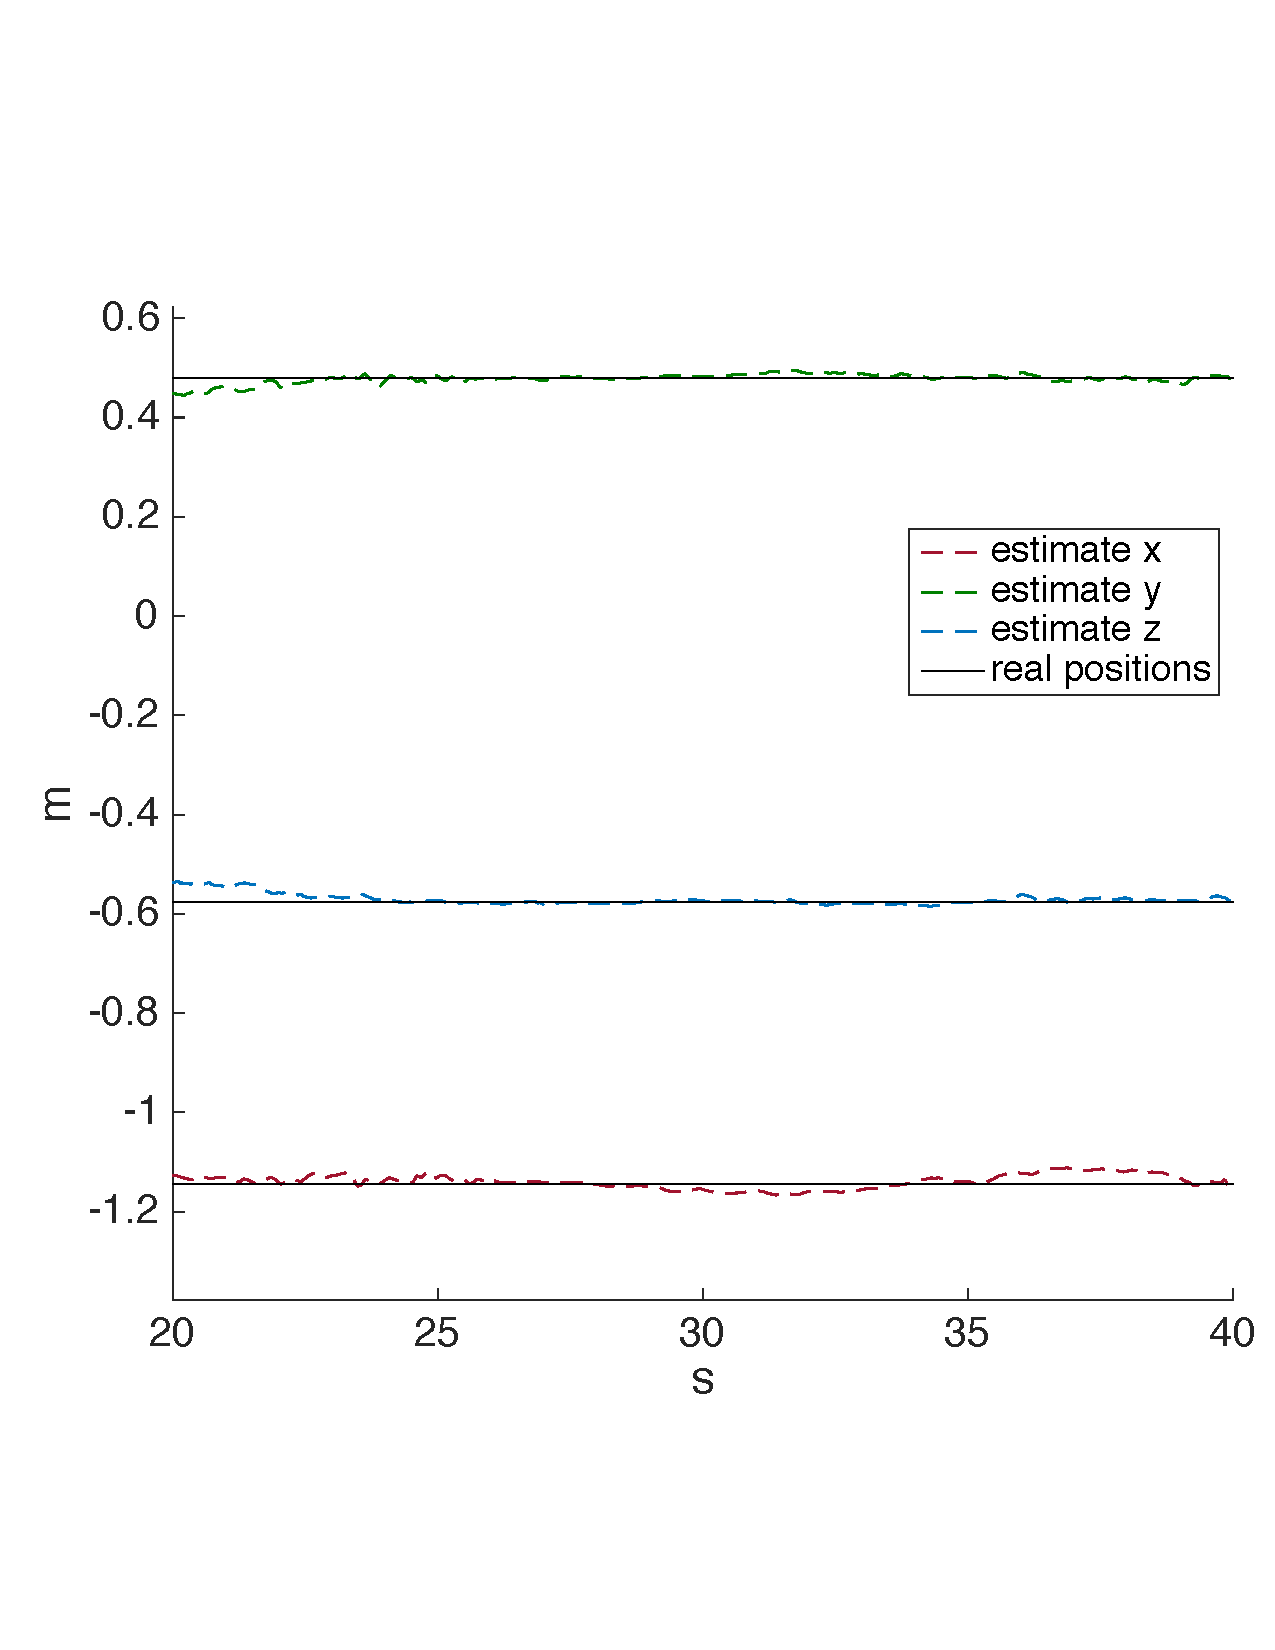
\includegraphics[width=\textwidth]{img/tag_static_real_world_pos.pdf}
        \caption{Position }
        \label{fig:one_ekf_real_world_static}
   \end{subfigure}\hfill
   \begin{subfigure}[b]{0.45\textwidth}
        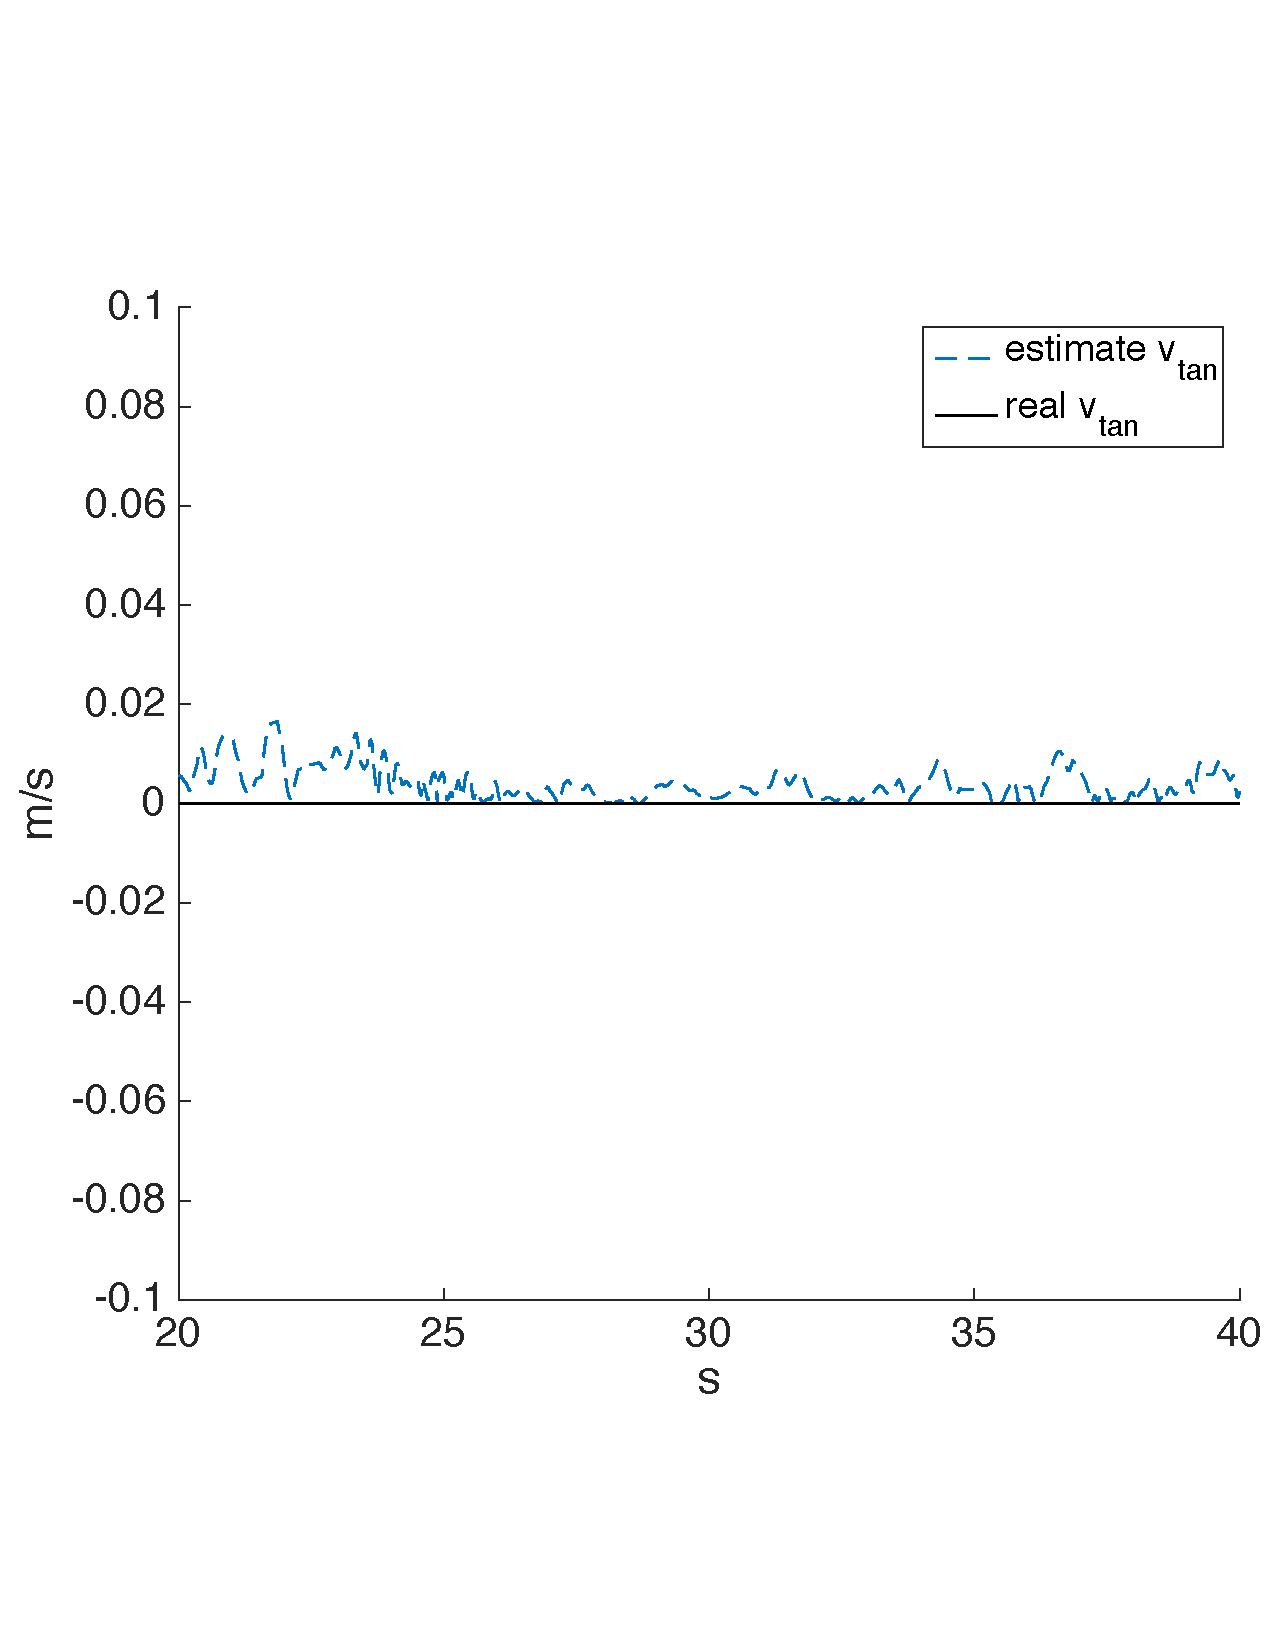
\includegraphics[width=\textwidth]{img/tag_static_real_world_vel.pdf}
        \caption{Velocity}
        \label{fig:two_ekf_real_world_static}
   \end{subfigure}
  \caption{Real world experiment. Comparison between estimate position and velocity with the ground truth values for a static platform. The estimate position has a RMSE of \SI{5}{\centi \meter} in $x,y$ and \SI{2.5}{\centi \meter} in $z$.}
  \label{fig:ekf_real_world_static}
\end{figure} 

\begin{figure}[!htbp]
  \centering
   \begin{subfigure}[b]{0.45\textwidth}
        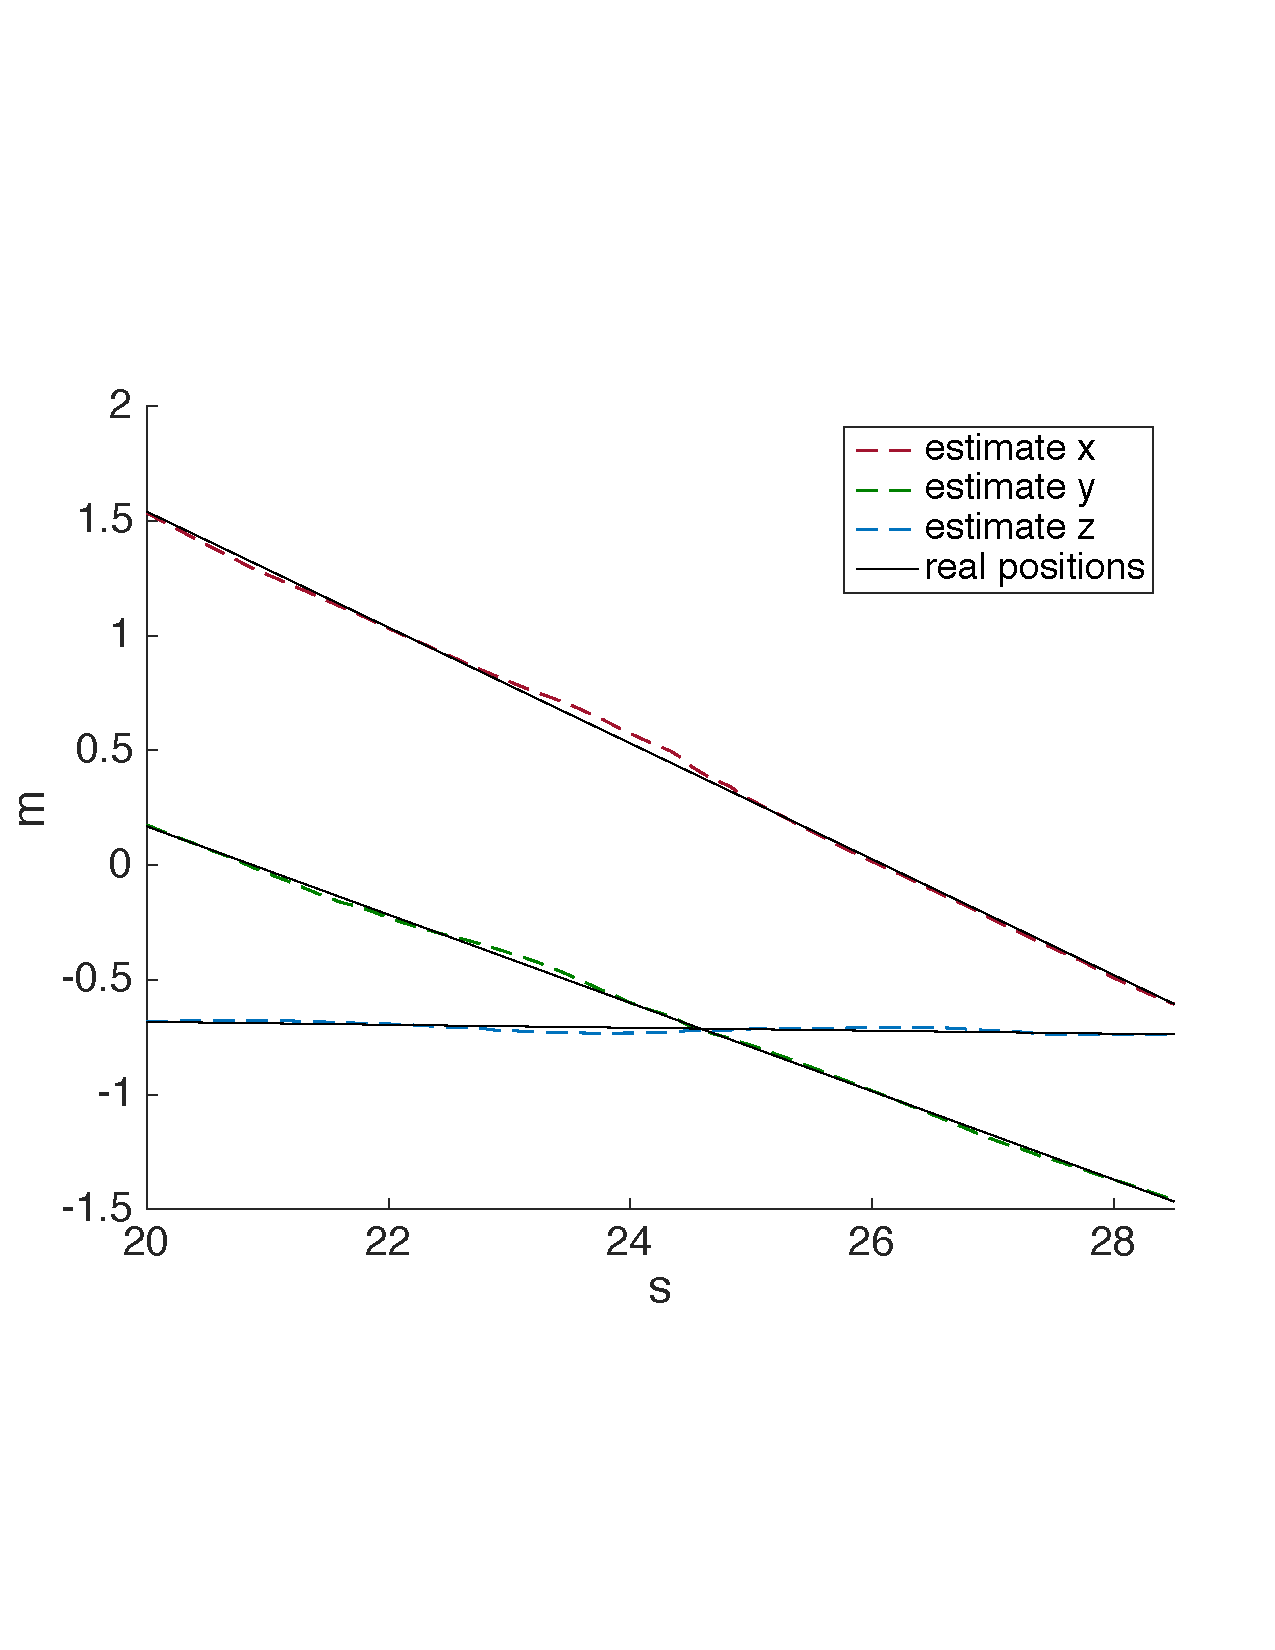
\includegraphics[width=\textwidth]{img/tag_moving_real_world_pos.pdf}
        \caption{Position }
        \label{fig:one_ekf_real_world_moving}
   \end{subfigure}\hfill
   \begin{subfigure}[b]{0.45\textwidth}
        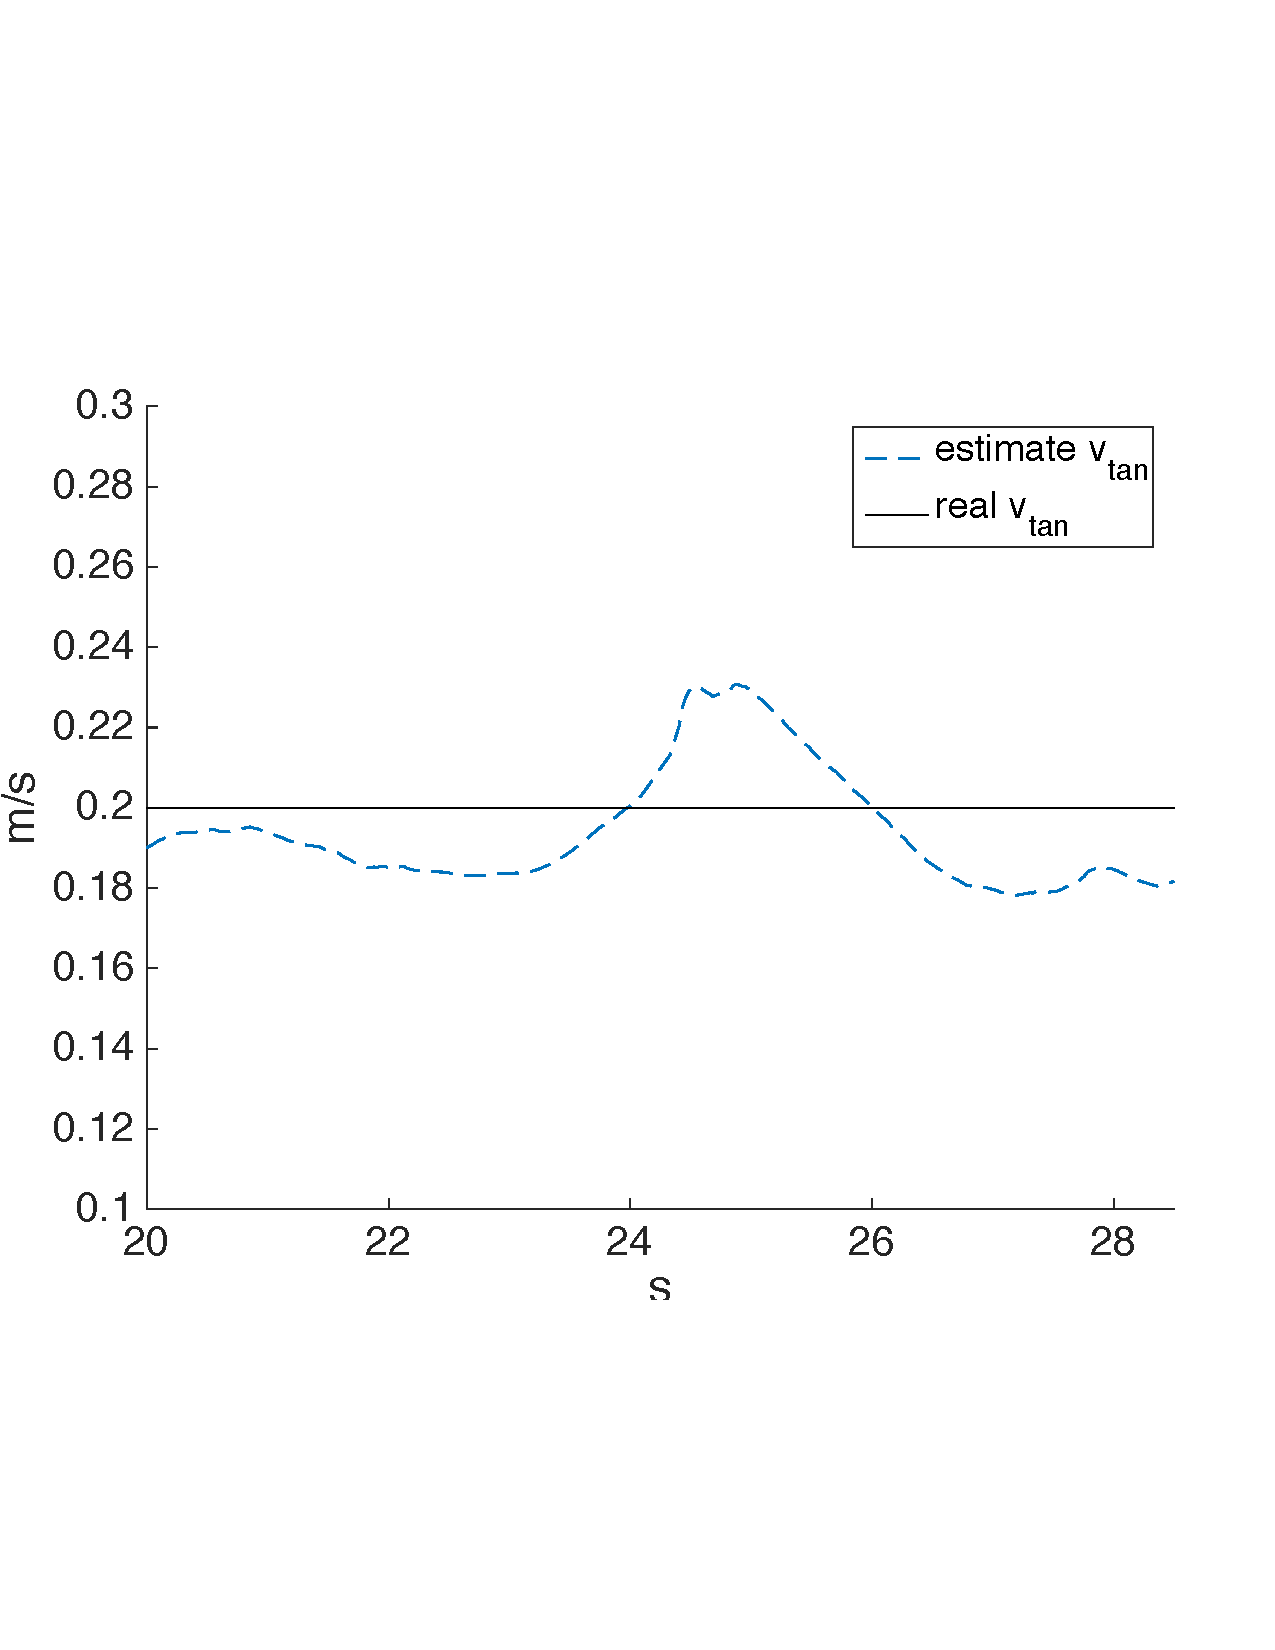
\includegraphics[width=\textwidth]{img/tag_moving_real_world_vel.pdf}
        \caption{Velocity \SI{0.2}{\meter \per \second}}
        \label{fig:two_ekf_real_world_moving}
   \end{subfigure}
    \centering
   \begin{subfigure}[b]{0.45\textwidth}
        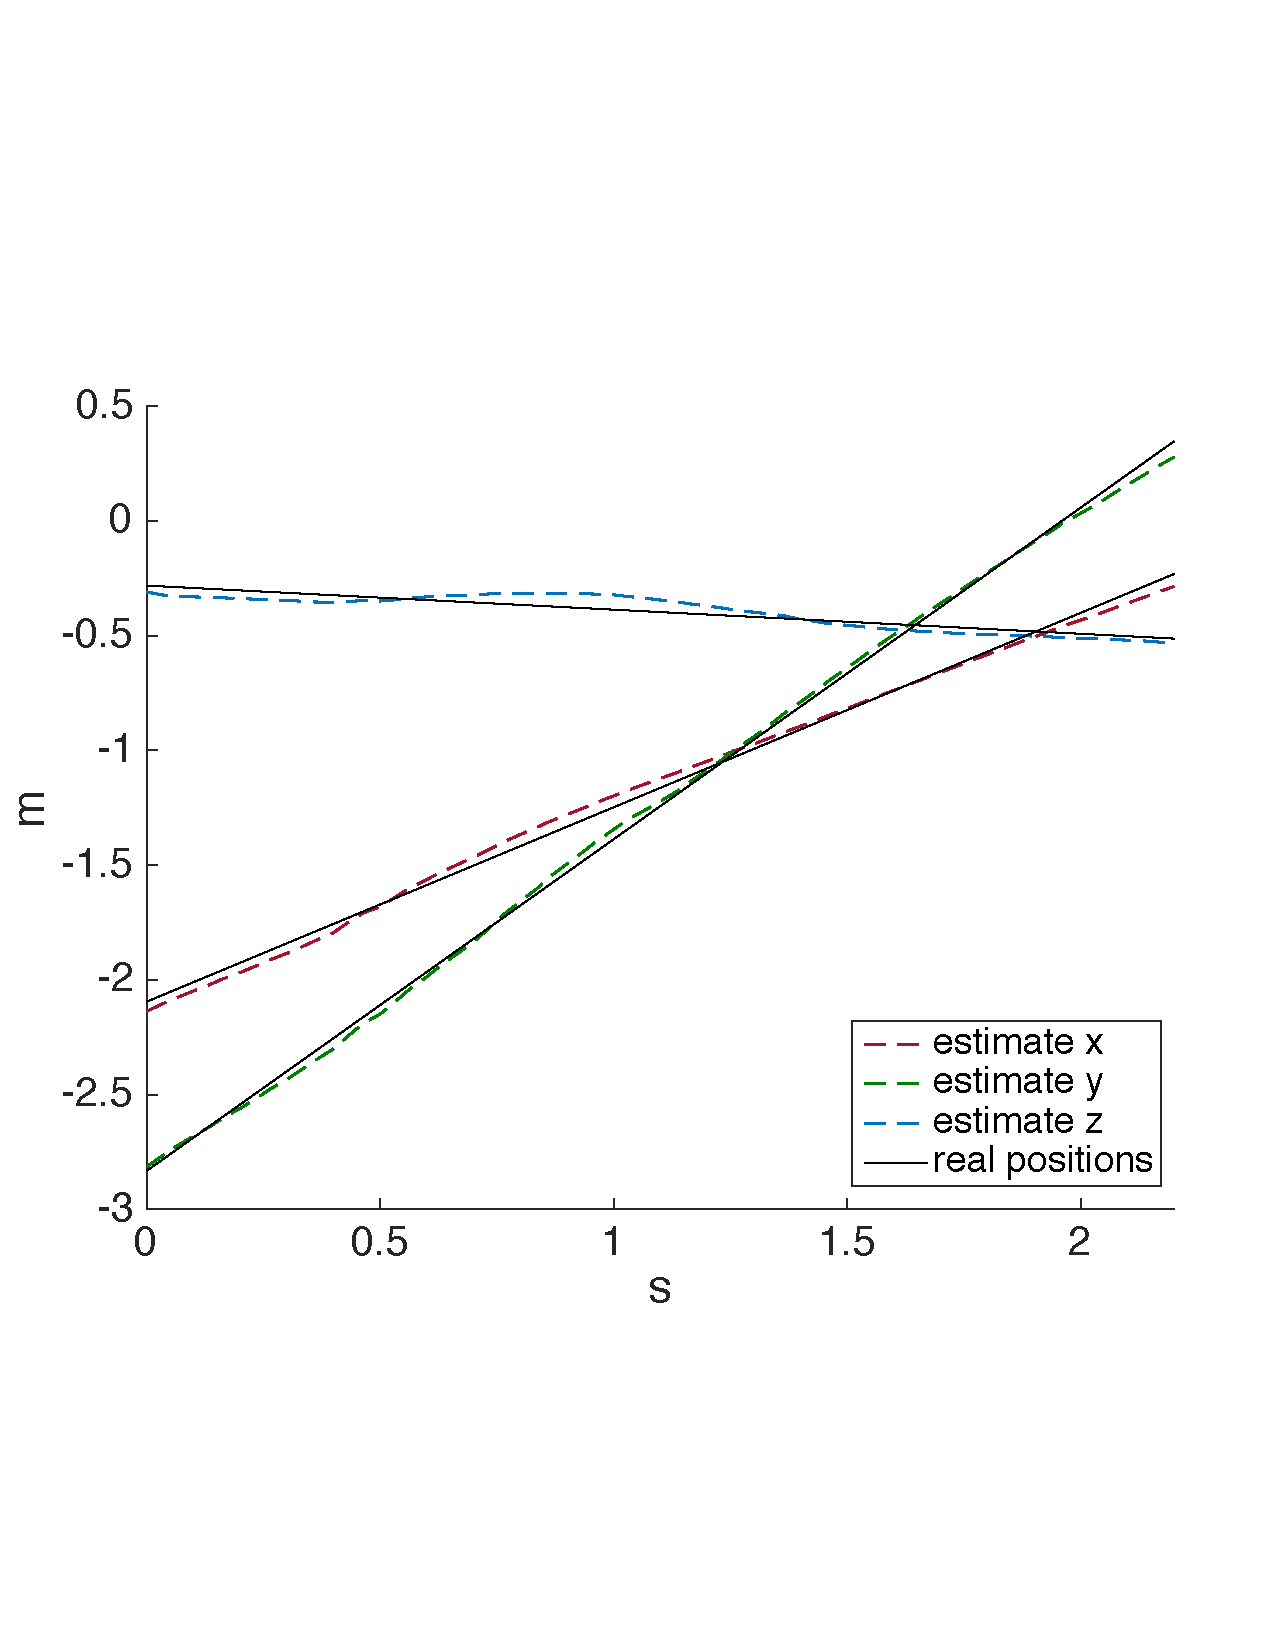
\includegraphics[width=\textwidth]{img/tag_moving_real_world_pos2.pdf}
        \caption{Position}
        \label{fig:one_ekf_real_world_moving2}
   \end{subfigure}\hfill
   \begin{subfigure}[b]{0.45\textwidth}
        \includegraphics[width=\textwidth]{img/tag_moving_real_world_vel2.pdf}
        \caption{Velocity  \SI{1.0}{\meter \per \second}}
        \label{fig:two_ekf_real_world_moving2}
   \end{subfigure}
  \caption{Real world experiment. Comparison between estimate position and velocity with the ground truth values for a platform moving at: figures (a)(b) \SI{0.2}{\meter \per \second}, figure (c)(d) \SI{1.0}{\meter \per \second}. The estimate position has a RMSE of \SI{3}{\centi \meter} in $x,y,z$.}
  \label{fig:ekf_real_world_moving}
\end{figure} 

\begin{figure}[!htbp]
  \centering
   \begin{subfigure}[b]{0.45\textwidth}
        \includegraphics[width=\textwidth]{img/tag_2ms_simulation_pos.pdf}
        \caption{Position }
        \label{fig:one_ekf_simulation_2ms}
   \end{subfigure}\hfill
   \begin{subfigure}[b]{0.45\textwidth}
        \includegraphics[width=\textwidth]{img/tag_2ms_simulation_vel.pdf}
        \caption{Velocity}
        \label{fig:two_ekf_simulation_2ms}
   \end{subfigure}
  \caption{Simulation test. Comparison between estimate position and velocity with the ground truth values. The velocity is initialized with a wrong value of \SI{1}{\meter \per \second} but the filter needs few steps to converge to the right value of \SI{2}{\meter \per \second}. The estimate position has a RMSE of \SI{10}{\centi \meter} in $x,y$ and \SI{2}{\centi \meter} in $z$.}
  \label{fig:ekf_simulation_2ms}
\end{figure} 


%\begin{figure}[!htbp]
%  \centering
%   \begin{subfigure}[b]{0.45\textwidth}
%        \includegraphics[width=\textwidth]{img/tag_2ms_simulation_pos.pdf}
%        \caption{Position }
%        \label{fig:one}
%   \end{subfigure}\hfill
%   \begin{subfigure}[b]{0.45\textwidth}
%        \includegraphics[width=\textwidth]{img/tag_2ms_simulation_vel.pdf}
%        \caption{Velocity}
%        \label{fig:two}
%   \end{subfigure}
%  \caption{Simulation test. Comparison between estimate position and velocity with the ground truth values. The velocity is initialized with 0 value. In this case the filter needs some time to converge to the right value of velocity.}
%  \label{fig:ekf_simulation_hot_init}
%\end{figure}


\section{Trajectory generation}

\subsection{Acceleration estimation} \label{subsec:acceleration_experiments}
We described in Sec.~\ref{subsec:acceleration} the three possible methods to estimate the acceleration of the quadrotor at a given time. This calculation is necessary because the trajectory generator needs a full state description of the initial condition of the quadrotor [position,velocity,acceleration] in order to solve the optimal control problem.\\
We took several datasets while the quadrotor was flying in the flyingroom in order to compare the different methods used to estimate the accelerations.\\

Figure~\ref{fig:comparison_acc} compares the accelerations estimated with IMU measurements, with finite difference calculated with two subsequent velocity estimations, and with the total thrust. On the left column we considered the raw data, while on the right column we consider the filtered versions of the accelerations calculated with finite difference and with the data from the IMU.
\begin{figure}[!htbp]
 \centering   
     \begin{subfigure}[b]{0.45\textwidth}
     \includegraphics[width=\textwidth]{img/acceleration_mass_changed_no_filter_x.pdf}
        \caption{Acceleration x axis not filtered}
        \label{fig:comparison_accx}
   \end{subfigure}
    \begin{subfigure}[b]{0.45\textwidth}
     \includegraphics[width=\textwidth]{img/acceleration_mass_changed_filtered_x.pdf}
        \caption{Acceleration x axis filtered}
        \label{fig:comparison_accx_fil}
   \end{subfigure}\\[20pt]
   
   \begin{subfigure}[b]{0.45\textwidth}
     \includegraphics[width=\textwidth]{img/acceleration_mass_changed_no_filter_y.pdf}
        \caption{Acceleration y axis  not filtered}
        \label{fig:comparison_accy}
   \end{subfigure}
    \begin{subfigure}[b]{0.45\textwidth}
     \includegraphics[width=\textwidth]{img/acceleration_mass_changed_filtered_y.pdf}
        \caption{Acceleration y axis filtered}
        \label{fig:comparison_accy_fil}
   \end{subfigure}\\[20pt]
   
    \begin{subfigure}[b]{0.45\textwidth}
     \includegraphics[width=\textwidth]{img/acceleration_mass_changed_no_filter_z.pdf}
        \caption{Acceleration z axis  not filtered}
        \label{fig:comparison_accz}
   \end{subfigure}
     \begin{subfigure}[b]{0.45\textwidth}
     \includegraphics[width=\textwidth]{img/acceleration_mass_changed_filtered_z.pdf}
        \caption{Acceleration z axis filtered}
        \label{fig:comparison_accz_fil}
   \end{subfigure}
    \caption{Comparison between the accelerations calculate with the three different methods. On the left side the raw data without filtering IMU and finite difference measurements. On the right column the same dataset, but with filtered version for IMU and finite difference.}
    \label{fig:comparison_acc}
\end{figure}

It is easy to notice that only the raw data from the thrust can be considered a good approximation of the acceleration, while the other two signals need some filtering. On the other hand, the filtered version of IMU and finite differences, are smooth but they have some delays.\\

Figure~\ref{fig:comparison_acc} shows that there is some offset between the three different approximations: in particular, in the z direction this difference between the acceleration computed with the thrust and the other two methods is very clear.\\
This offset is more evident in the Fig.~\ref{fig:comparison_acc_mass} where the right graph is the same Fig.~\ref{fig:comparison_accz_fil}, while the left part is calculate with the same data set, but the mass of the quadrotor is modify by the $5\%$ from \SI{515}{\gram} to \SI{545}{\gram}. This tiny modification is creating a big difference in the final acceleration.

\begin{figure}[!htbp]
 \centering   
  \begin{subfigure}[b]{0.45\textwidth}
     \includegraphics[width=\textwidth]{img/acceleration_mass_correct_filtered_z.pdf}
        \caption{Acceleration z axis filtered with real mass of 545g}
        \label{fig:comparison_accz_mass}
   \end{subfigure}
     \begin{subfigure}[b]{0.45\textwidth}
     \includegraphics[width=\textwidth]{img/acceleration_mass_changed_filtered_z.pdf}
        \caption{Acceleration z axis filtered with modify mass of 515g}
        \label{fig:comparison_accz_fil_mass}
   \end{subfigure}
    \caption{Comparison between the accelerations calculate with the three different methods. On the left side accelerations calculate considering the real mass of 545g , on the right column considering 545g}
    \label{fig:comparison_acc_mass}
\end{figure}

Also in the other axis, if we change the mass, we can see that the acceleration estimation computed with the thrust shows an offset with respect to the other two signals.\\ This could be caused by a not precise estimation of the rotor fitness factors.\\

\section{Landing on a moving platform}
We also made different trials of the entire framework, in order to understand if all the pieces linked together are good enough to complete the task.\\
In simulation we reached velocity of the moving platform of up to \SI{3}{\meter \per \second}, while in the real world we managed to achieve velocity of \SI{0.6}{\meter \per \second} for the platform. \\
We achieved a successful landing rate of over $90\%$.\\
The main issues why we have not tried yet higher velocity in the real world is that the quadrotor we are using has hardware limitations that do not allow fast trajectory tracking, so in the final stages of the state machine, the trajectory generator is not able to find feasible trajectories that bring the quadrotor on the platform. Furthermore, the trajectory replanning at high velocities causes some fast oscillations to the quadrotor, and this may result the failure of the visual odometry. 

Figs. \ref{fig:landing1},  \ref{fig:landing2} and  \ref{fig:landing3}  show pictures from different tests in the real world and in simulation. In each set of pictures we highlighted the stages of the landing state machine. The quadrotor proceeds from a stage to another until it completes the mission and lands on the moving platform.

\begin{figure}[!htbp]
  \centering
   \begin{subfigure}[b]{0.45\textwidth}
        \includegraphics[width=\textwidth]{img/takeoff3.jpg}
        \caption{Takeoff.}
   \end{subfigure}\hfill
   \begin{subfigure}[b]{0.45\textwidth}
        \includegraphics[width=\textwidth]{img/exploring3.jpg}
        \caption{Exploration.}
        \label{fig:two}
   \end{subfigure}\hfill
    \begin{subfigure}[b]{0.45\textwidth}
        \includegraphics[width=\textwidth]{img/following3.jpg}
        \caption{Following the base.}
        \label{fig:three}
   \end{subfigure}\hfill
    \begin{subfigure}[b]{0.45\textwidth}
        \includegraphics[width=\textwidth]{img/approaching3.jpg}
        \caption{Approaching the base.}
        \label{fig:three}
   \end{subfigure}\hfill
   \begin{subfigure}[b]{0.45\textwidth}
        \includegraphics[width=\textwidth]{img/align3.jpg}
        \caption{Align with the base.}
        \label{fig:three}
   \end{subfigure}\hfill
    \begin{subfigure}[b]{0.45\textwidth}
        \includegraphics[width=\textwidth]{img/landing3.jpg}
        \caption{Landing on the base.}
        \label{fig:four}
   \end{subfigure} \hfill
    \begin{subfigure}[b]{0.45\textwidth}
        \includegraphics[width=\textwidth]{img/landed3.jpg}
        \caption{Landed on the base.}
        \label{fig:five}
   \end{subfigure}
   
  \caption{Sequence of images taken from a simulation experiment in which the platform is moving at \SI{2.0}{\meter \per \second} }
  \label{fig:landing1}
\end{figure}

\begin{figure}[!htbp]
  \centering
   \begin{subfigure}[b]{0.5\textwidth}
        \includegraphics[width=\textwidth]{img/takeoff2.jpg}
        \caption{Takeoff.}
   \end{subfigure}
   \begin{subfigure}[b]{0.5\textwidth}
        \includegraphics[width=\textwidth]{img/exploring2.jpg}
        \caption{Exploration.}
        \label{fig:two}
   \end{subfigure}
   \begin{subfigure}[b]{0.5\textwidth}
        \includegraphics[width=\textwidth]{img/align2.jpg}
        \caption{Align with the base.}
        \label{fig:three}
   \end{subfigure}
    \begin{subfigure}[b]{0.5\textwidth}
        \includegraphics[width=\textwidth]{img/landing2.jpg}
        \caption{Landing on the base.}
        \label{fig:four}
   \end{subfigure} 
    \begin{subfigure}[b]{0.5\textwidth}
        \includegraphics[width=\textwidth]{img/landed2.jpg}
        \caption{Landed on the base.}
        \label{fig:five}
   \end{subfigure}
   
  \caption{Sequence of images taken from a real world experiment in which the platform is moving at \SI{0.5}{\meter \per \second} }
  \label{fig:landing2}
\end{figure} 

\begin{figure}[!htbp]
  \centering
   \begin{subfigure}[b]{0.5\textwidth}
        \includegraphics[width=\textwidth]{img/takeoff1.jpg}
        \caption{Takeoff.}
   \end{subfigure}
   \begin{subfigure}[b]{0.5\textwidth}
        \includegraphics[width=\textwidth]{img/exploring1.jpg}
        \caption{Exploration.}
        \label{fig:two}
   \end{subfigure}
   \begin{subfigure}[b]{0.5\textwidth}
        \includegraphics[width=\textwidth]{img/align1.jpg}
        \caption{Align with the base.}
        \label{fig:three}
   \end{subfigure}
    \begin{subfigure}[b]{0.5\textwidth}
        \includegraphics[width=\textwidth]{img/landing1.jpg}
        \caption{Landing on the base.}
        \label{fig:four}
   \end{subfigure} 
    \begin{subfigure}[b]{0.5\textwidth}
        \includegraphics[width=\textwidth]{img/landed1.jpg}
        \caption{Landed on the base.}
        \label{fig:five}
   \end{subfigure}
   
  \caption{Sequence of images taken from a real world experiment in which the platform is moving at \SI{0.6}{\meter \per \second} }
  \label{fig:landing3}
\end{figure} 




 

%\begin{figure}[h]
%   \centering
%   \includegraphics[width=0.75\textwidth]{img/processing_time.pdf}
%   \caption{Example of a figure.}
%   \label{img:timing}
%\end{figure}

%\chapter{Scientific Writing}\label{chap:scietific_wiritng}

This chapter gives you some tips on how to write scientifically. It should prevent you from making the most common mistakes people do and help you with creating a well written report.

\section{General Style}

\begin{itemize}
	\item A report/paper is not a short-story. There is no build-up to a climax. The climax should be in the abstract. Even better, in the title.
	\item Hierarchical exposition, not linear: this goes in hand with the previous point.
	A hierarchical exposition means that you start with the core of your work (The main thing your project was about) and then go into details in following sections.
	Do not build up to the core of your work with too much background/preliminaries as it would be the case in a linear exposition.
	\item At the beginning of every chapter/major section, you should summarize what the content of the section will be.
	A person should get a good sense of the report by reading the first paragraph of each section.
	\item Express your thoughts succinctly.
	Avoid unnecessary words or phrases and be precise and specific.
	\item Definitions are useful if they are used often.
	Do not define something if it is only used once.
	\item Be generous with your references.
	Do not compare your results with others by pointing the deficiencies of their work; rather, state how your results are adding to the body of knowledge others have created.
	\item Notation is extremely important.
	Good notation facilitates understanding. You do not want the reader to mentally perform translations every time they see a symbol.
\end{itemize}

\section{Important Stuff}

\begin{itemize}
	\item Use active verb tense whenever possible: instead of \emph{An analysis of the signal noise is performed using a discrete Fourier transform.} write \textbf{We perform an analysis of the signal noise using a discrete Fourier transform.}
	\item Make short sentences with one statement. 
	Long sentences with multiple statements are complicated and hard to understand. 
	Write to be understood, not to impress!
	\item Be concrete/specific: instead of \emph{We use a model to predict the state} write \textbf{We use a linear model of the attitude dynamics to predict the quadrotor's state at time $t + \Delta t$}.
	\item Be precise: instead of \emph{We assume the model to be linear}, say \textbf{We design a linear model of the system dynamics}. (You assume the \emph{system dynamics} to be linear and hence you create a linear model.)
	\item Be consistent: this basically applies to every level. Denote the same thing always with the same word, create figures with a similar style, etc.
	\item Do not make unsubstantiated statements.
	Do not use \emph{It is common knowledge} or \emph{Several researchers have shown}.
	Instead use constructs like \textbf{Recently, several researchers~\cite{KleinMurray2007,Strasdat2010WhyFilter} have shown}.
\end{itemize}

\section{Small Things}

\begin{itemize}
	\item Do not use \emph{don't}, \emph{aren't}, etc., use \textbf{do not} and \textbf{are not}.
	\item Do not use words like \emph{simply}, \emph{highly}, \emph{just}, \emph{very}, etc.
	\item Use \textbf{because} instead of \emph{due to the fact that}, \textbf{to} instead of \emph{in order to}, etc.
	\item When referencing to figures, sections, etc., use capital letters: see \textbf{Figure}~1, see \textbf{Section}~2.
	\item Every figure must be referenced in the text.
	\item Use $\sim$ to make spaces which \LaTeX\ must not separate: Figure$\sim$\textbackslash\texttt{ref\{fig:bla\}}.
	This avoids having the word and the number on different lines.
	\item Put punctuation marks after each formula as if they were text. 
	Separate multiple consecutive formulas by commas and put a dot if you start a new sentence after the formula.
	For more details, see Section~\ref{sec:math}.
	\item Use \textbackslash\texttt{left(} and \textbackslash\texttt{right)} when you have mathematical expressions that are higher than normal brackets, e.g., $\left(\frac{pV}{RT}\right)$ instead of $(\frac{pV}{RT})$.
	\item Avoid brackets. If something is important enough to be mentioned it does not need brackets; if not, it does not need to be mentioned at all.
	\item In English, after a colon (:) you continue with small letters.
	\item Use \emph{we} to refer to yourself, i.e. \textbf{We} developed an algorithm to ...
	\item Do not use \emph{ours}.
	\item Number all equations.
	\item Put details in an appendix.
	\item Avoid single-sentence paragraphs.
\end{itemize}
%\chapter{\LaTeX\ Tips and Tricks}\label{chap:tipstricks}

In this chapter, we show some useful tips and tricks when working with \LaTeX.

\section{Using Git}

We recommend you to use \emph{Git} also for your \LaTeX\ files such as this report.
If you do so, we suggest to write every sentence in your \TeX\ file on a new line.
This will make it easier to keep track of changes since \emph{Git} tracks them line by line.
So if you change one sentence, \emph{Git} will tell you that only that sentence has changed instead of the entire paragraph otherwise.
Furthermore, if you are using the PDF viewer of \emph{texmaker}, you can jump from the PDF directly to the sentence in the \TeX\ file by clicking on it (instead of just jumping to the corresponding paragraph).

\section{Headings}

Your report can be structured using several different types of headings.
Use the commands \textbackslash\texttt{chapter}\{.\}, \textbackslash\texttt{section}\{.\}, \textbackslash\texttt{subsection}\{.\}, and \textbackslash\texttt{subsubsection}\{.\}.
Use the asterisk symbol \texttt{*} to suppress numbering of a certain heading if necessary, for example, \textbackslash\texttt{section*}\{.\}.


\section{References}\label{sec:references}

References to literature are included using the command \textbackslash\texttt{cite}\{$\cdot$\}.
For example \cite{KleinMurray2007,Strasdat2010WhyFilter}.
Your references must be entered in the file \texttt{bibliography.bib}.
Making changes or adding new references in the bibliography file can be done manually or by using specialized software such as \textit{JabRef} which is free of charge.

Cross-referencing within the text is easily done using \textbackslash\texttt{label}\{$\cdot$\} and \textbackslash\texttt{ref}\{$\cdot$\}.
For example, this paragraph is part of Chapter~\ref{chap:tipstricks}; more specifically on page~\pageref{sec:references}.

\section{Writing Equations}\label{sec:math}

The most common way to include equations is using the \texttt{equation} environment.
Use \textbackslash\texttt{eqref}\{$\cdot$\} to reference an equation, e.g., \eqref{eq:pose_candidates}.

Embed equations in the text.
Thus you must use proper punctuation.
You must introduce all symbols that you use.
You should define these before you use them.
However, they must be introduced in the same sentence at the latest. 

\subsection*{Example 1}

For $n$ detections and $m$ LEDs on the object, we will
obtain $N$ pose candidates,
% (this is to avoid extra space)
	\begin{equation}\label{eq:pose_candidates}
		N =  4 \alpha \binom{n}{3} \frac{m!}{(m-3)!},
	\end{equation}
% (this is to avoid extra space)
where $\alpha \in \left\{ {1, 2}\right\}$ is a magic factor.

\subsection*{Example 2}

The transformation matrix in homogeneous coordinates, $\mathtt{T}$, is composed of the rotation matrix $\mathbf{R}$ and translation vector $\mathbf{p}$,
% (this is to avoid extra space)
  \begin{equation}\label{eq:se3}
    \mathtt{T} = \begin{bmatrix}\mathbf{R} & \mathbf{p} \\ 0 & 1\end{bmatrix}, \qquad \text{with} \quad \mathbf{R} \in SO(3), \ \ \mathbf{p} \in \mathbb{R}^3.
  \end{equation}


\section{Including Graphics}\label{sec:epsgraph}

The easiest way to include figures in your document is to use PDF figures if you use \texttt{pdflatex} to compile.
Figure \ref{img:notation} was created with the use of the open-source program \texttt{ipe}.

  \begin{figure}[h]
     \centering
     \includegraphics[width=0.6\textwidth]{img/notation.pdf}
     \caption{Example of a figure.}
     \label{img:notation}
  \end{figure}

\section{Including Matlab Figures}

When including figures into your report you want them as a vector graphic such that you can zoom into the figure without getting blurry.
Furthermore it is nice when the text in the figure gets substituted by \LaTeX\ such that you have the same font and the same font size.
Figure \ref{fig:example_tikz_figure} shows an example of such an imported matlab figure.
An easy way of achieving this is by using the \texttt{matlab2tikz} script.
You can find a short example on how to use this script in the \texttt{matlab\_figures} folder.
The \texttt{create\_figures.m} script creates a plot and then the tikz file which you can include in your document.
For using tikz, you need to make use of the \texttt{pgfplots} package in your \TeX\ document.
More information on using \texttt{matlab2tikz} can be found on \href{http://www.mathworks.com/matlabcentral/fileexchange/22022-matlab2tikz}{Matlab Central} where you can also download the necessary files (\texttt{matlab2tikz.m}, \texttt{matlab2tikzInputParser.m}, \texttt{updater.m}).

\begin{figure}[H]
  \centering
  \setlength\fwidth{8.0cm}
  \setlength\fheight{6.0cm}
  % This file was created by matlab2tikz v0.4.7 running on MATLAB 8.0.
% Copyright (c) 2008--2014, Nico Schlömer <nico.schloemer@gmail.com>
% All rights reserved.
% Minimal pgfplots version: 1.3
% 
% The latest updates can be retrieved from
%   http://www.mathworks.com/matlabcentral/fileexchange/22022-matlab2tikz
% where you can also make suggestions and rate matlab2tikz.
% 
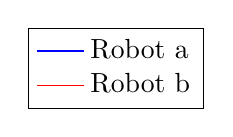
\begin{tikzpicture}

\begin{axis}[%
width=\fwidth,
height=\fheight,
scale only axis,
xmin=0,
xmax=10,
xlabel={time [$s$]},
ymin=-1,
ymax=1,
ylabel={velocity [$\frac{m}{s}$]},
legend style={draw=black,fill=white,legend cell align=left}
]
\addplot [color=blue,solid]
  table[row sep=crcr]{0	0\\
0.101010101010101	0.100838420258105\\
0.202020202020202	0.200648856522685\\
0.303030303030303	0.298413804447641\\
0.404040404040404	0.39313661214833\\
0.505050505050505	0.483851640437935\\
0.606060606060606	0.569634106908966\\
0.707070707070707	0.649609513505707\\
0.808080808080808	0.72296256147946\\
0.909090909090909	0.788945462844257\\
1.01010101010101	0.846885563602983\\
1.11111111111111	0.896192201029956\\
1.21212121212121	0.936362725104285\\
1.31313131313131	0.9669876227093\\
1.41414141414141	0.987754692360084\\
1.51515151515152	0.998452226900389\\
1.61616161616162	0.998971171723357\\
1.71717171717172	0.98930623651434\\
1.81818181818182	0.969555949182324\\
1.91919191919192	0.939921651430131\\
2.02020202020202	0.900705446202955\\
2.12121212121212	0.852307117939675\\
2.22222222222222	0.795220057023049\\
2.32323232323232	0.730026229976446\\
2.42424242424242	0.657390246682775\\
2.52525252525253	0.578052585106573\\
2.62626262626263	0.492822042588923\\
2.72727272727273	0.402567490669497\\
2.82828282828283	0.308209017490077\\
2.92929292929293	0.210708548077192\\
3.03030303030303	0.11106003812413\\
3.13131313131313	0.0102793412405343\\
3.23232323232323	-0.0906061470334077\\
3.33333333333333	-0.190567962875485\\
3.43434343434343	-0.288587058720432\\
3.53535353535354	-0.383664191806112\\
3.63636363636364	-0.474830110822239\\
3.73737373737374	-0.561155436815202\\
3.83838383838384	-0.641760137619388\\
3.93939393939394	-0.71582249922919\\
4.04040404040404	-0.782587502654202\\
4.14141414141414	-0.84137452086087\\
4.24242424242424	-0.89158425733514\\
4.34343434343434	-0.932704855531834\\
4.44444444444444	-0.964317116928778\\
4.54545454545455	-0.98609877449093\\
4.64646464646465	-0.997827777979213\\
4.74747474747475	-0.999384557612436\\
4.84848484848485	-0.990753243005677\\
4.94949494949495	-0.972021824958833\\
5.05050505050505	-0.943381258446\\
5.15151515151515	-0.905123515950137\\
5.25252525252525	-0.857638610988052\\
5.35353535353535	-0.80141062216897\\
5.45454545454545	-0.737012758318913\\
5.55555555555556	-0.665101514978822\\
5.65656565656566	-0.586409981847235\\
5.75757575757576	-0.501740369393911\\
5.85858585858586	-0.411955830830862\\
5.95959595959596	-0.317971662810619\\
6.06060606060606	-0.220745974555063\\
6.16161616161616	-0.121269920537167\\
6.26262626262626	-0.0205575962872592\\
6.36363636363636	0.0803642996702817\\
6.46464646464646	0.180466932359911\\
6.56565656565657	0.278729818677557\\
6.66666666666667	0.37415123057122\\
6.76767676767677	0.465758407025652\\
6.86868686868687	0.552617470746406\\
6.96969696969697	0.633842948448906\\
7.07070707070707	0.708606797699218\\
7.17171717171717	0.776146848283581\\
7.27272727272727	0.835774572052259\\
7.37373737373737	0.886882102029079\\
7.47474747474747	0.928948429231251\\
7.57575757575758	0.961544714026824\\
7.67676767676768	0.984338657883824\\
7.77777777777778	0.997097890943875\\
7.87878787878788	0.999692340886112\\
7.97979797979798	0.992095558932323\\
8.08080808080808	0.974384989475536\\
8.18181818181818	0.946741180583354\\
8.28282828282828	0.909445943424462\\
8.38383838383838	0.862879479381784\\
8.48484848484848	0.807516504139563\\
8.58585858585859	0.743921408256844\\
8.68686868686869	0.672742503562265\\
8.78787878787879	0.594705414024498\\
8.88888888888889	0.510605678474283\\
8.98989898989899	0.421300640588607\\
9.09090909090909	0.327700708813498\\
9.19191919191919	0.230760075325052\\
9.29292929292929	0.131466988642958\\
9.39393939393939	0.030833679061141\\
9.49494949494949	-0.0701139604006468\\
9.5959595959596	-0.170346832328096\\
9.6969696969697	-0.268843125910384\\
9.7979797979798	-0.364598733655889\\
9.8989898989899	-0.456637487633774\\
10	-0.54402111088937\\
};
\addlegendentry{Robot a};

\addplot [color=red,solid]
  table[row sep=crcr]{0	1\\
0.101010101010101	0.99490281585683\\
0.202020202020202	0.9796632259997\\
0.303030303030303	0.954436588420145\\
0.404040404040404	0.919480072752278\\
0.505050505050505	0.875150038590823\\
0.606060606060606	0.82189840263017\\
0.707070707070707	0.760268031659151\\
0.808080808080808	0.690887208377067\\
0.909090909090909	0.614463226448467\\
1.01010101010101	0.531775180091039\\
1.11111111111111	0.443666021702229\\
1.21212121212121	0.35103396849205\\
1.31313131313131	0.254823345726049\\
1.41414141414141	0.156014959925759\\
1.51515151515152	0.0556161001658067\\
1.61616161616162	-0.0453497306018852\\
1.71717171717172	-0.145853249514135\\
1.81818181818182	-0.244869886685079\\
1.91919191919192	-0.341390230048921\\
2.02020202020202	-0.434430315678286\\
2.12121212121212	-0.523041658674875\\
2.22222222222222	-0.606320922373835\\
2.32323232323232	-0.683419127290403\\
2.42424242424242	-0.753550305929445\\
2.52525252525253	-0.815999515227557\\
2.62626262626263	-0.870130124945965\\
2.72727272727273	-0.915390307713636\\
2.82828282828283	-0.951318664558728\\
2.92929292929293	-0.97754892857964\\
3.03030303030303	-0.993813698804694\\
3.13131313131313	-0.999947166176124\\
3.23232323232323	-0.995886803868673\\
3.33333333333333	-0.981674004711079\\
3.43434343434343	-0.957453659212335\\
3.53535353535354	-0.923472678494476\\
3.63636363636364	-0.880077477189673\\
3.73737373737374	-0.827710441961886\\
3.83838383838384	-0.76690542165429\\
3.93939393939394	-0.69828228503756\\
4.04040404040404	-0.62254060163933\\
4.14141414141414	-0.54045251007479\\
4.24242424242424	-0.452854846581271\\
4.34343434343434	-0.360640614001448\\
4.44444444444444	-0.264749878183483\\
4.54545454545455	-0.166160184603552\\
4.64646464646465	-0.0658765929072468\\
4.74747474747475	0.0350785690386048\\
4.84848484848485	0.135676127132719\\
4.94949494949495	0.234890552819178\\
5.05050505050505	0.331710417703216\\
5.15151515151515	0.425148704424772\\
5.25252525252525	0.514252868676963\\
5.35353535353535	0.598114549793553\\
5.45454545454545	0.67587883091213\\
5.55555555555556	0.746752954311448\\
5.65656565656566	0.810014403075603\\
5.75757575757576	0.865018266697566\\
5.85858585858586	0.911203815534403\\
5.95959595959596	0.948100217091764\\
6.06060606060606	0.975331335863734\\
6.16161616161616	0.992619567796701\\
6.26262626262626	0.999788670287321\\
6.36363636363636	0.996765558864523\\
6.46464646464646	0.983581052239521\\
6.56565656565657	0.960369558128524\\
6.66666666666667	0.927367703050975\\
6.76767676767677	0.884911920071669\\
6.86868686868687	0.833435019078179\\
6.96969696969697	0.773461774557475\\
7.07070707070707	0.705603575851525\\
7.17171717171717	0.630552194429187\\
7.27272727272727	0.54907273171308\\
7.37373737373737	0.461995819353901\\
7.47474747474747	0.37020915146548\\
7.57575757575758	0.274648435144047\\
7.67676767676768	0.176287851525489\\
7.77777777777778	0.0761301246240719\\
7.87878787878788	-0.0248037008054478\\
7.97979797979798	-0.125484668174093\\
8.08080808080808	-0.224886398621082\\
8.18181818181818	-0.321995554297938\\
8.28282828282828	-0.415822168707717\\
8.38383838383838	-0.505409738788067\\
8.48484848484848	-0.589844975855707\\
8.58585858585859	-0.668267116007629\\
8.68686868686869	-0.739876695065317\\
8.78787878787879	-0.80394369860703\\
8.88888888888889	-0.859815004003662\\
8.98989898989899	-0.906921038591359\\
9.09090909090909	-0.944781586105027\\
9.19191919191919	-0.973010682179788\\
9.29292929292929	-0.991320549013866\\
9.39393939393939	-0.99952452908148\\
9.49494949494949	-0.997538987988408\\
9.5959595959596	-0.985384167071799\\
9.6969696969697	-0.963183977052532\\
9.7979797979798	-0.931164734843692\\
9.8989898989899	-0.889652856392602\\
10	-0.839071529076452\\
};
\addlegendentry{Robot b};

\end{axis}
\end{tikzpicture}%
  \caption{Example figure created with \texttt{matlab2tikz}.}
  \label{fig:example_tikz_figure}
\end{figure}

An alternative which you might want to consider is \texttt{matlabfrag} and \texttt{mlf2pdf}.
Especially when there are many data points in your figure you might run into problems when using tikz.
Again, you can find a short example on how to use \texttt{mlf2pdf} in the \texttt{create\_figures.m} scriptin in the \texttt{matlab\_figures} folder.
This script makes use of the two functions \texttt{matlabfrag.m} and \texttt{mlf2pdf.m} to create a PDF which you can then include into matlab.
These two files can be downloaded \href{http://www.mathworks.ch/matlabcentral/fileexchange/28545-matlabfrag-to-pdf}{here} and \href{http://www.mathworks.ch/matlabcentral/fileexchange/21286-matlabfrag}{here}.

\begin{figure}[H]
     \centering
     \includegraphics[width=0.85\textwidth]{matlab_figures/example_matlabfrag_figure.pdf}
     \caption{Example figure created with \texttt{mlf2pdf}.}
     \label{fig:example_matlab_fig}
  \end{figure}


\section{Including Code in your Document}

You may include samples from your Matlab code using the \texttt{lstlistings} environment, for example:

  \lstset{language=Matlab,numbers=none}
  \begin{lstlisting}[frame=lines, caption=Matlab Example, label=matlabexample]
  % Evaluate y = 2x
  for i = 1:length(x)

    y(i) = 2*x(i);

  end
  \end{lstlisting}

  \lstset{language=C++,numbers=none,caption=C++ Example, label=cppexample}
  \begin{lstlisting}[frame=lines]
  // sum all elements in a list
  int sum=0;
  for(list<int>::iterator it=mylist.begin(); it!=mylist.end(); ++it)
    sum += *it;
  \end{lstlisting}

%\chapter{RPG Notation Style}\label{chap:notation}

This chapter presents some conventions on notation that we use at the Robotics and Perception Group.
Try to stick to those conventions since a unique style makes it easier to review the report.

\section{Variable styles in \LaTeX}

Use lowercase and bold letters for vectors, e.g. $\textbf{x}$, uppercase and bold letters for matrices, e.g. $\textbf{R}$, and lowercase letters with normal weight for scalars, e.g. $s$.

\section{Coordinate Systems and Rotations}

We use the notation introduced by Prof. Glocker in the course ``Mechanik 3'' at ETHZ to express coordinate frames, rotations and vectors.
Refer to Chapter~5 ``Kinematik'' in the lecture script for more details \footnote{\url{http://mitschriften.amiv.ethz.ch/main.php?page=3&scrid=1&pid=87&eid=1}}.
Figure \ref{fig:notation} gives an overview of how coordinate transformations and vectors are specified.
Observe that the coordinate system in which a vector is expressed is always written as index before the variable, e.g. $_B\mathbf{t}_{AB}$ is the vector from $A$ to $B$ expressed the coordinate system $B$.
For the ease of reading, the index for the origin coordinate frame can be omitted: $_O\mathbf{t}_k := \mathbf{t}_k$.

\begin{figure}[H]
     \centering
     \includegraphics[scale=0.8]{img/notation}
     \caption{Notation overview.}
     \label{fig:notation}
\end{figure}
  
$A$ and $B$ are two adjacent coordinate frames and $O$ is the frame of origin.
$\mathbf{R}_{AB}$ describes the coordinate transformation from frame $B$ to frame $A$, thus it holds that 
	\[
		\begin{aligned}
			_O\mathbf{t}_k  &= \mathbf{R}_{OB} \ _B\mathbf{f}_k, \\
			\mathbf{R}_{OB} &= \mathbf{R}_{OA} \ \mathbf{R}_{AB}.
	  \end{aligned} 
	\]

\section{Measured, estimated and target values}

For controllers and estimators please specify the variables as follows in the report:

	\[
		\begin{aligned}
			\text{true value:} \quad & \mathbf{x} \\
			\text{estimated value:} \quad & \hat{\mathbf{x}} \\
			\text{measured value:} \quad & \tilde{\mathbf{x}} \\
			\text{desired value:} \quad & \mathbf{x}_\text{des} \\
      \text{error value:} \quad & \mathbf{x}_\text{e} \\
      \text{equilibrium value:} \quad & \mathbf{x}^* \\
		\end{aligned}
	\]

\chapter{Discussion}\label{chap:discussion}

TODO
Explain both the advantages and limitations of your approach.

\section{Conclusion}\label{sec:conclusion}
In this thesis we presented a complete framework to permits a quadrotor to find, approach and land on a moving platform. We explained all the modules that make up the system, showing in detail the computation we perform in order to complete the assigned task. \\
Several experiments were carried in simulation and in the real world to demonstrate the functionality of our system. From these experiments we demonstrate robustness of the framework up to a certain velocity, after which the trajectory generation and the self state estimation modules start to fail.\\

\section{Future Work}\label{sec:future_work}
There are several upgrades that can be done to this frameworks. The major problems are related to the not always robust state estimation and the issues with the trajectory generator ( described in \ref{sec:trajectory_problem}).\\
 Following we describe what solution can be applied in future to solve these problems.

\subsection{State estimation using also GPS and Teraranger}
A future upgrade that we should do is to fuse multiple sensor to have a more robust and precise state estimation.\\
As a matter of fact MSF can combine easily different sources of data, filtering them with the IMU information.
The main two sensor we can add for this upgrade can be:
\begin{itemize}
\item GPS: it gives a 3D absolute position with not a high accuracy, but are always available in outside environment, and can be useful to have a continue state estimation used to initialized (and reinitialized if it fails) the visual odometry. Of course the uncertainty related to this measure will be much more higher w.r.t the one from SVO, but it is MSF's duty taking in account these information and filtering the data in the right way.
\item Teraranger \cite{teraranger}: it is distance sensor for robotics, it can operate both in inside and outside environment, it is very light and can be really useful to have an estimation of the height of the quadrotor. It is in fact well known that both VO and GPS systems have much more error in the depth component, so the data from this sensor can be correct all the wrong estimations from the other two sources. 
\end{itemize}

\subsection{Change the controller}
As describe before the trajectory generator has some issues that must be resolved \label{sec:trajectory_problem}. The approach to solve these problems can be:
\begin{itemize}
\item make the flight controller more sensitive: right now the replanning does not work because the first desired state of the trajectory is too close to the current state to generate a correct control action. Making the controller more response at little variation can solve this problem.\\
A method to increase the sensitivity is tuning the controller gains, but this can lead to a unstable behavior, so further studies must be done.
\item change both the trajectory and the contorller: implementing a new contorller like a LQR controller \cite{wiki_lqr} that takes in account both the dynamic of the quad and the platform and directly calculate the control actions necessary to arrive at a certain final state.\\  In this case the state machine should not predict in advance where the platform will be in $T$ seconds because this prediction is directly done by the LQR controller. The main problem with this type of controller is tuning the weights in the cost function to have a nice and smooth flight. \\ 
Furthermore we can implement a continuous replanning of the control actions of the LQR, leading with an MPC framework. This solution, as described in the introduction of the thesis, is really computational expensive and before implementing it, we must understand if it can run onboard on our quadrotor.
\end{itemize} 

\subsection{Cross detector}
In the final challenge the moving platform will be signed with the marker in figure \ref{fig:finalplatform}. \\
In order to have a measurement update in the low-altitude EKF we have to implement a cross detector: instead of estimating the 4dof pose of the platform from the AR-tag detection, we must be able to extract the same information from the cross mark.\\

The detector itself should not be really hard to implement  (it consists in a new Pnp problem) the only problem can be due to the symmetry of the cross that does not allow to detect a unique solution for the yaw orientation. On the other end once we are estimating the initial yaw angle we are able to detect correctly the changing in orientation, as far as between two consecutive measures the platform rotates a few degrees: we cannot distinguish between rotations of $k90^o$, but we know that two measures close in time has also close degree because the angular velocity of the platform is not really high.\\

From the point of view of our framework we can simply substitute the detection module and everything still working: this new detector should provide the same data of the AR-tag detector used in this thesis, and so it can directly be used as update step on the EKF already implemented.\\

\cleardoublepage

% Appendix______________________________________________________________________
\appendix
%\chapter{Something}\label{sec:something}

In the appendix, you can provide some more data, a tutorial on how to run your code, a detailed proof, etc.

It is, however, not a requirement to have an appendix.

\cleardoublepage

% Bibliography__________________________________________________________________

\bibliographystyle{unsrt}
\bibliography{bibtex/references.bib}

\end{document}
